\documentclass[fontset=none]{Notes}

\makeatletter
\DeclareRobustCommand{\em}{%
  \@nomath\em \if b\expandafter\@car\f@series\@nil
  \normalfont \else \bfseries \fi}
\makeatother

\usepackage{tikz-cd,wrapstuff}
\usepackage{fixdif,siunitx,tikz,nicematrix}
\usetikzlibrary{matrix,calc}

\ProvidesFile{font.def}

\setCJKmainfont{Source Han Serif SC}[
  UprightFont=*-Regular,
  BoldFont=*-Bold,
  ItalicFont=HYKaiTi S,
  ItalicFeatures={Scale=1.1}
]
\newCJKfontfamily[zhsong]\songti{Source Han Serif SC}[
  UprightFont=*-Regular,
  BoldFont=*-Bold,
  ItalicFont=HYKaiTi S,
  ItalicFeatures={Scale=1.1}
]
\setCJKsansfont{Source Han Sans SC}[
  UprightFont=*-Regular,
  BoldFont=*-Bold
]
\newCJKfontfamily[zhhei]\heiti{Source Han Sans SC}[
  UprightFont=*-Regular,
  BoldFont=*-Bold
]
\setCJKmonofont{HYFangSong S}[
  BoldFont=*,
  ItalicFont=*,
  BoldItalicFont=*
]
\newCJKfontfamily[zhfs]\fangsong{HYFangSong S}[
  BoldFont=*,
  ItalicFont=*,
  BoldItalicFont=*
]
\newCJKfontfamily[zhkai]\kaishu{HYKaiTi S}[
  BoldFont=*,
  ItalicFont=*,
  BoldItalicFont=*
]

\setmainfont{texgyretermes}[
  Extension=.otf,
  UprightFont=*-regular,
  BoldFont=*-bold,
  ItalicFont=*-italic,
  BoldItalicFont=*-bolditalic,
  SlantedFont=*-italic
]
%\setmathrm{texgyretermes}[
%  Extension=.otf,
%  UprightFont=*-regular,
%  BoldFont=*-bold,
%  ItalicFont=*-italic,
%  BoldItalicFont=*-bolditalic,
%  SlantedFont=*-italic
%]
\setsansfont{Cantarell}[
  UprightFont=* Regular,
  ItalicFont=* Italic,
  BoldFont=* Bold,
  BoldItalicFont=* Bold Italic,
  SmallCapsFont=Alegreya Sans SC
]
\setmonofont{Ubuntu Mono}[
  UprightFont=*,
  ItalicFont=* Italic,
  BoldFont=* Bold,
  BoldItalicFont=* Bold Italic
]
%\setmathfont{texgyretermes-math.otf}
%\setmathfont[range={\mathcal,\mathbfcal,\mathfrak},StylisticSet=1]{XITSMath-Regular.otf}
%\setmathfont[range={\mathbb}]{KpMath-Sans.otf}



\usepackage[subscriptcorrection,nofontinfo,mtpbb,mtpfrak]{mtpro2}

\tikzcdset{
  arrow style=tikz,
  diagrams={>={Straight Barb[scale=0.8]}}
}

\allowdisplaybreaks[1]

\newlength{\mymathln}
\newcommand{\aligninside}[2]{
  \settowidth{\mymathln}{#2}
  \mathmakebox[\mymathln]{#1}
}

\DeclareMathOperator\Spec{Spec}
\DeclareMathOperator\im{im}
\DeclareMathOperator\nil{nil}
\DeclareMathOperator\rad{rad}
\DeclareMathOperator\Ann{Ann}
\DeclareMathOperator\Max{Max}
\DeclareMathOperator\End{End}
\DeclareMathOperator\Tor{Tor}
\DeclareMathOperator\Frac{Frac}
\DeclareMathOperator\Tr{Tr}
\DeclareMathOperator\Hom{Hom}
\DeclareMathOperator\coker{coker}

\newcommand{\ideal}[1]{\mathfrak{#1}}
\newcommand{\mat}[1]{\mathbold{#1}}
\newcommand{\uline}{\underline{\hphantom{X}}}

\usepackage{enumitem}

\setlist[enumerate]{nosep}

%\DeclareMathAlphabet\mathcal{OMS}{cmsy}{m}{n}

\newlength\stextwidth
\newcommand\makesamewidth[3][c]{%
  \settowidth{\stextwidth}{#2}%
  \makebox[\stextwidth][#1]{#3}%
}



\begin{document}

\frontmatter

\tableofcontents

\mainmatter

\chapter{环和理想}

\begin{theorem}[Jumping's typology theorem]
  令 $\mathcal{W}$ 是手写求和符号范畴。$\mathcal{W}$ 中存在唯一的对象 $\frac{\infty}{2}$
  (Jumping 符号)和一族 typo 态射 $\sum^{(\cdot)}\to\frac{\infty}{2}$。对于每个 $\mathcal{W}$
  中对象到正确求和符号的态射 $\sum^{(\cdot)}\to\sum^\infty$(称为反 typo 态射),存在
  唯一的从 Jumping 符号 $\frac{\infty}{2}$ 到正确求和符号 $\sum^{\infty}$ 的态射使得下面的
  图表交换:
  \[
    \begin{tikzcd}[column sep=huge,row sep=huge]
      \sum^{(\cdot)} \arrow[dr,"\mathrm{anti-typo}"',sloped]\arrow[r,"\mathrm{typo}"]
      &
      \frac{\infty}{2} \arrow[d,"\mathrm{correct}",sloped] \\
      &
      \sum^{\infty}
    \end{tikzcd}
  \]
\end{theorem}

\section{素理想和极大理想}

在本课程中,“环”一词始终指的是一个有单位元 $1$ 的交换环。

\begin{definition}
  $A$ 是一个环,$A$ 的所有素理想的集合称为 $A$ 的\emph{谱},记为 $\Spec(A)$。
  $A$ 的所有极大理想的集合称为 $A$ 的\emph{极大谱},记为 $\Omega(A)$。
\end{definition}

$f:A\to B$ 是一个环同态,对于每个 $\ideal{q}\in\Spec(B)$,考虑复合同态
$g=\pi\circ f:A\to B/\ideal{q}$,那么 $\ker g=f^{-1}(\ideal{q})$,故
$A/f^{-1}(\ideal q)\simeq \im g\subset B/\ideal q$ 是整环,所以
$f^{-1}(\ideal q)\in\Spec(A)$,故 $f$ 诱导出了映射 $f^*:\Spec(B)\to\Spec(A)$,
$f^*(\ideal q)=f^{-1}(\ideal q)$。对于极大理想并没有类似的结果,
例如 $A=\mathbb{Z},B=\mathbb{Q}$,映射 $f:A\to B$ 为嵌入映射,取 $B$ 的极大理想 $0$,
但是 $f^{-1}(0)=0$ 不是 $A$ 的极大理想。

再提一下理想 $\ideal p$ 是素理想的三个重要等价条件,这三种后面都会用到:
\begin{enumerate}
  \item 定义:若 $ab\in\ideal p$,则 $a\in\ideal p$ 或者 $b\in\ideal p$;
  \item 逆否命题:若 $a\notin\ideal p$ 且 $b\notin\ideal p$,则 $ab\notin\ideal p$;
  \item 写为理想的形式:若理想 $\ideal a,\ideal b$ 满足 $\ideal a\ideal b\subseteq\ideal p$,
  则 $\ideal a\subseteq\ideal p$ 或者 $\ideal b\subseteq\ideal p$。
\end{enumerate}

\begin{theorem}
  任意非零环 $A$ 至少有一个极大理想。
\end{theorem}
\begin{proof}
  令 $S$ 为 $A$ 中所有不等于 $(1)$ 的理想的集合。由于 $(0)\in S$,所以 $S$ 非空。
  在集合的包含关系下 $S$ 成为一个偏序集。对于 $S$ 中的每个链 $T$,考虑
  \[
    I=\bigcup_{\ideal a\in T}\ideal a , 
  \]
  容易验证 $I$ 是不等于 $(1)$ 的理想,所以 $I\in S$ 是 $T$ 的上界。那么
  根据 Zorn 引理,$S$ 存在一个极大元 $\ideal{m}$。若理想 $J$ 满足,
  $\ideal m\subseteq J\subseteq A$,如果 $J\neq A$,那么 $J\in S$,由于
  $\ideal m$ 是极大元,所以 $J=\ideal m$,故 $\ideal m$ 就是一个极大理想。
\end{proof}

\begin{corollary}\label{coro:non-zero ideal is contained in a maximal ideal}
  如果 $\ideal a\neq (1)$ 是 $A$ 的一个理想,那么存在一个包含 $\ideal a$ 的极大理想。
\end{corollary}
\begin{proof}
  $A/\ideal a$ 是非零环,从而至少有一个极大理想,对应于 $A$ 的包含 $\ideal a$ 的极大理想。
\end{proof}

\begin{corollary}
  $A$ 的任意非单位元素 $a$ 都被包含在一个极大理想中。
\end{corollary}

\begin{definition}
  若环 $A$ 只有一个极大理想 $\ideal m$,那么 $A$ 被称为\emph{局部环}。
  对应的域 $A/\ideal m$ 被称为\emph{$A$ 的剩余域}。
\end{definition}

\begin{example}
  \mbox{}
  \begin{enumerate}
    \item 任意域都是局部环,其只有一个极大理想 $0$。
    \item $p$ 是素数,$\mathbb{Z}/p^n\mathbb{Z}$ 是局部环,其极大理想
    为 $p\mathbb{Z}/p^n\mathbb{Z}$。这是因为 $\mathbb{Z}/p^n\mathbb{Z}$ 的极大理想
    一一对应到 $\mathbb{Z}$ 中包含 $(p^n)$ 的极大理想 $(a)$,
    那么 $a\mid p^n$,由于 $\mathbb{Z}$ 是主理想整环,所以 $(a)$ 是极大理想当且仅当
    $a$ 是不可约元,故只有 $a=p$,对应于 $p\mathbb{Z}/p^n\mathbb{Z}$。
    \item 域 $F$ 上的形式幂级数环 $F[[x]]$ 是局部环,其极大理想为
    $(x)$。注意到如果 $a_0+a_1x+a_2x^2+\cdots \notin (x)$,即 $a_0\neq 0$,
    那么
    \[
      \frac{1}{a_0+a_1x+a_2x^2+\cdots}  
      =
      \frac{1}{a_0}\frac{1}{1+(a_1/a_0x+a_2/a_0x^2+\cdots)}
      =\frac{1}{a_0}(1-a_1/a_0x+\cdots),
    \]
    这表明 $a_0+a_1x+a_2x^2+\cdots$ 是单位。另一方面,
    因为 $x$ 不可逆,所以 $(x)$ 中的元素都不可逆。故 $F[[x]]$ 的单位群
    就是 $F[[x]]\backslash (x)$。这表明若 $\ideal a\neq (1)$ 是理想,那么
    必然有 $\ideal a\subseteq (x)$。这就表明 $(x)$ 是唯一的极大理想。
  \end{enumerate}
\end{example}

上述例 3 可以进行一般化,即下面的命题。

\begin{proposition}
  \mbox{}
  \begin{enumerate}
    \item $A$ 是一个环,$\ideal m\neq (1)$ 是一个理想,并且任意 $x\in A\backslash\ideal m$
    都是 $A$ 中的单位,那么 $A$ 是局部环,且 $\ideal m$ 为 $A$ 的极大理想。
    \item $A$ 是一个环,$\ideal m$ 是一个极大理想,使得 $1+\ideal m$ 中的每个元素
    都是 $A$ 中的单位,那么 $A$ 是局部环。
  \end{enumerate}
\end{proposition}
\begin{proof}
  (1) 任意 $x\in A\backslash\ideal m$ 都是 $A$ 中的单位表明若 $\ideal a\neq (1)$
  是任意理想,那么 $\ideal a\subseteq \ideal m$,所以 $\ideal m$ 是唯一的极大理想。

  (2) 任取 $x\in A\backslash\ideal m$,那么 $x+\ideal m\in A/\ideal m$ 是非零元,所以
  存在 $y+\ideal m\in A/\ideal m$ 使得 $(x+\ideal m)(y+\ideal m)=1+\ideal m$,
  即 $xy-1\in\ideal m$,故 $xy\in 1+\ideal m$ 是单位,所以 $x$ 是单位,由 (1)
  可知 $A$ 是局部环。
\end{proof}

\section{幂零根和 Jacobson 根}

\begin{proposition}
  环 $A$ 的所有幂零元的集合 $\nil(A)$ 是一个理想,并且
  $A/\nil(A)$ 没有非零的幂零元。
\end{proposition}
\begin{proof}
  任取 $x\in\nil(A)$,显然对于所有的 $a\in A$,$ax$ 仍然是幂零元。
  任取 $x,y\in\nil(A)$,即存在 $m,n$ 使得 $x^m=0,y^n=0$,那么
  \[
    (x-y)^{m+n}=\sum_{i=0}^{m+n}\binom{m+n}{i}x^i(-y)^{m+n-i}  
    =\left(\sum_{i=0}^m +\sum_{i=m+1}^{m+n}\right)\binom{m+n}{i}x^i(-y)^{m+n-i}  ,
  \]
  前一个和式的每一项中 $m+n-i\geq n$,故 $x^i(-y)^{m+n-i}=0$,
  后一个和式的每一项中 $i\geq m$,故 $x^i(-y)^{m+n-i}=0$,
  所以 $x-y\in\nil(A)$,即 $\nil(A)$ 是一个理想。

  若 $a+\nil(A)$ 是幂零元,即存在 $m$ 使得 $a^m+\nil(A)=0$,
  即 $a^m\in\nil(A)$,这表明 $a\in\nil(A)$。
\end{proof}

\begin{definition}
  理想 $\nil(A)$ 被称为 $A$ 的\emph{幂零根}。
\end{definition}

\begin{proposition}
  $A$ 的幂零根是所有素理想的交集。
\end{proposition}
\begin{proof}
  令 $\nil'(A)$ 是 $A$ 的所有素理想的交集。如果 $a\in A$ 是幂零元,
  那么存在 $m$ 使得 $a^m=0\in\ideal p$,$\ideal p$ 是任意素理想。根据素理想的定义,
  这表明 $a\in\ideal p$,故 $a\in\nil'(A)$。

  另一方面,如果 $a\in A$ 不是幂零元,令 $S$ 是理想 $\ideal a$ 的集合,
  $\ideal a$ 满足对于任意的 $n>0$,$a^n\notin\ideal a$。由于 $0\in S$,
  所以 $S$ 非空。容易验证 $S$ 满足 Zorn 引理使用条件,所以存在极大元 $\ideal p$。
  我们证明 $\ideal p$ 是素理想。若 $x,y\notin\ideal p$,那么
  $\ideal p+(x)$ 和 $\ideal p+(y)$ 严格包含 $\ideal p$,因此它们不属于
  $S$,于是存在 $m,n$ 使得
  \[
    a^m\in\ideal p+(x),\quad a^n\in\ideal p+(y).
  \]
  这表明 $a^{m+n}\in (\ideal p+(x))(\ideal p+(y))\subseteq \ideal p+(xy)$,
  故 $\ideal p+(xy)\notin S$,所以 $xy\notin\ideal p$。这表明 $\ideal p$
  是素理想。所以存在一个素理想 $\ideal p$ 使得 $a\notin\ideal p$,故
  $a\notin\nil'(A)$。
\end{proof}

\begin{definition}
  环 $A$ 的所有极大理想的交集被称为 $A$ 的\emph{Jacobson 根},记为 $\rad(A)$。
\end{definition}

\begin{proposition}\label{prop:Jacobson radical}
  $x\in \rad(A)$ 当且仅当对于任意的 $y\in A$,$1-xy$ 是单位。
\end{proposition}
\begin{proof}
  若 $x\in \rad(A)$,那么对于任意的 $y\in A$ 有 $xy\in \rad(A)$。 
  如果 $1-xy$ 不是单位,那么存在一个极大理想 $\ideal m\ni 1-xy$,
  注意到 $xy\in \rad(A)\subseteq \ideal m$,所以 $1=(1-xy)+xy\in \ideal m$,
  这与 $\ideal m$ 是极大理想矛盾,所以 $1-xy$ 是单位。

  若对于任意的 $y\in A$, $1-xy$ 是单位。假设存在一个极大理想 $\ideal m$
  使得 $x\notin\ideal m$,故 $\ideal m+(x)$ 严格包含 $\ideal m$,
  所以 $(1)=\ideal m+(x)$,即存在 $y\in A$ 使得 $1=m+xy$,其中 $m\in\ideal m$,
  那么 $1-xy=m$ 不是单位,推出矛盾。故 $x\in \rad(A)$。
\end{proof}

\section{幂等元与环的分解}

这部分是上课的内容,书中没有。
环 $A$ 中满足 $x^2=x$ 的元素被称为幂等元。$0$ 和 $1$ 显然是幂等元,被称为平凡幂等元。
关于幂等元可以注意到下面的两个简单事实:如果 $x$ 是幂等元,那么 $(1-x)^2=1-2x+x^2=1-x$,
所以 $1-x$ 也是幂等元,并且 $x(1-x)=0$。如果 $x\in A^\times$ 是幂等元,那么 $x=x^2x^{-1}=xx^{-1}=1$,
所以 $A^\times$ 中的幂等元只有 $1$。

\begin{definition}
  一个环 $A$ 如果不能同构于两个非零环 $A_1$ 和 $A_2$ 的直积,那么称
  $A$ 是\emph{不可分解的}。
\end{definition}

幂等元实际上和环的可分解性联系紧密,体现在下面的引理。

\begin{lemma}
  $A$ 是一个环,那么下面的说法是等价的:
  \begin{enumerate}
    \item 存在两个非零环 $A_1,A_2$ 使得 $A\simeq A_1\times A_2$;
    \item $A$ 存在非平凡幂等元;
    \item 存在两个非零理想 $\ideal a_1,\ideal a_2$ 使得 $A=\ideal a_1\oplus\ideal a_2$。
  \end{enumerate}
\end{lemma}
\begin{proof}
  $(1)\Rightarrow (2)$ 如果存在两个非零环 $A_1,A_2$ 使得 $A\simeq A_1\times A_2$,
  那么 $(0,0),(1,0),(0,1)$ 是 $A_1\times A_2$ 的三个幂等元,所以 $A_1\times A_2$ 一定有
  非平凡幂等元,即 $A$ 存在非平凡幂等元。

  $(2)\Rightarrow (3)$ 如果 $A$ 存在非平凡幂等元 $e$,注意到任意的 $x\in A$ 满足
  $x=xe+x(1-e)$,所以 $A=(e)+(1-e)$。取 $x\in (e)\cap (1-e)$,那么存在
  $a,b\in A$ 使得 $x=ae=b(1-e)$,那么 $ae=ae^2=b(1-e)e=0$,所以 $x=0$。
  这就表明 $A=(e)\oplus (1-e)$。

  $(3)\Rightarrow (1)$ 考虑同态 $\phi:A\to A/\ideal a_1\times A/\ideal a_2$,
  $\phi(x)=(x+\ideal a_1,x+\ideal a_2)$,由于 $\ker\phi=\ideal a_1\cap\ideal a_2=0$,
  所以 $\phi$ 是单射。任取 $(x+\ideal a_1,y+\ideal a_2)\in A/\ideal a_1\times A/\ideal a_2$,
  设 $1=a_1+a_2$,其中 $a_1\in \ideal a_1,a_2\in\ideal a_2$,那么
  令 $a=xa_2+ya_1$,就有
  \[
    \phi(a)=(xa_2+\ideal a_1,ya_1+\ideal a_2)  
    =(x+\ideal a_1,y+\ideal a_2),
  \]
  所以 $\phi$ 是满射,故 $A\simeq A/\ideal a_1\times A/\ideal a_2$。
\end{proof}

\begin{example}
  \mbox{}
  \begin{enumerate}
    \item 整环都是不可分解的,因为 $x^2-x=x(x-1)=0$ 的解只有 $0$ 和 $1$。
    \item 局部环是不可分解的,若 $x$ 是一个非平凡幂等元,那么 $1-x$ 可逆,从而 $1-x=1$,
    即 $x=0$,这与 $x$ 非平凡矛盾。
  \end{enumerate}
\end{example}



\section{理想的操作}

对于环 $A$ 的两个理想 $\ideal a,\ideal b$,有 
$(\ideal a+\ideal b)(\ideal a\cap\ideal b)
=\ideal a(\ideal a\cap\ideal b)+\ideal b(\ideal a\cap \ideal b)\subseteq \ideal 
a\ideal b\subseteq\ideal a\cap\ideal b$,这表明 $\ideal a+\ideal b=(1)$ 的时候,
有 $\ideal a\cap\ideal b=\ideal a\ideal b$,我们将这种情况称为 $\ideal a$ 与 $\ideal b$
互素。

$A$ 是环,$\ideal a_1,\dots,\ideal a_n$ 是 $A$ 的理想,定义同态
\[
  \phi:A\to\prod_{i=1}^n (A/\ideal a_i)
\]
为 $\phi(x)=(x+\ideal a_1,\dots,x+\ideal a_n)$。

下面的命题实际上就是中国剩余定理的证明。

\begin{proposition}
  \mbox{}
  \begin{enumerate}
    \item 若 $\ideal a_i,\ideal a_j$ 互素($i\neq j$),那么 $\prod\ideal a_i=\bigcap \ideal a_i$。
    \item $\phi$ 是满射当且仅当 $i\neq j$ 的时候总有 $\ideal a_i,\ideal a_j$ 互素。
    \item $\phi$ 是单射当且仅当 $\bigcap\ideal a_i=(0)$。
  \end{enumerate}
\end{proposition}
\begin{proof}
  (1) 对 $n$ 归纳即可。$n=2$ 的时候上面已经说明,假设结论在 $n-1$ 的时候成立。
  我们证明 $\ideal a_i$ 和 $\prod_{j\neq i}\ideal a_j$ 互素即可。这实际上是证明
  若理想 $\ideal a_1,\ideal a_2$ 都和 $\ideal b$ 互素,那么 $\ideal a_1\ideal a_2$
  也和 $\ideal b$ 互素。注意到
  \[
    (1)=(\ideal a_1+\ideal b)(\ideal a_2+\ideal b)
    \subseteq \ideal a_1\ideal a_2+\ideal a_1\ideal b
    +\ideal b\ideal a_2+\ideal b  \subseteq
    \ideal a_1\ideal a_2+\ideal b,
  \]
  这就表明 $\ideal a_1\ideal a_2$ 与 $\ideal b$ 互素。
  回到这个命题,重复上述步骤就可以得到 $\ideal a_i$ 和 $\prod_{j\neq i}\ideal a_j$ 互素,
  根据假设,$\prod_{j\neq i}\ideal a_j=\bigcap_{j\neq i}\ideal a_j$,
  故
  \[
    \prod_{i=1}^n \ideal a_i
    =\ideal a_i\left(\prod_{j\neq i} \ideal a_j\right)  
    =\ideal a_i\cap\left(\prod_{j\neq i} \ideal a_j\right)  
    =\ideal a_i\cap\left(\bigcap_{j\neq i}\ideal a_j\right)
    =\bigcap_{i=1}^n\ideal a_i.
  \]

  (2) 若 $\phi$ 是满射,对于 $(0,\dots,1+\ideal a_i,\dots,0)$,
  存在 $a\in A$,使得 $\phi(a)=(0,\dots,1+\ideal a_i,\dots,0)$,
  这表明 $1-a\in\ideal a_i$,并且 $a\in\ideal a_j\ (j\neq i)$,故
  \[
    1=  (1-a)+a\in \ideal a_i+\ideal a_j,
  \]
  这就表明 $\ideal a_i$ 和 $\ideal a_j$ 互素。

  反之,若 $\ideal a_i$ 和 $\ideal a_j$ 互素。令 $\ideal b_i=\prod_{j\neq i}\ideal a_j$,
  那么 $\ideal b_1+\ideal b_2=(\ideal a_2+\ideal a_1)\ideal a_3\cdots\ideal a_n=\ideal a_3\cdots\ideal a_n$,
  进一步的,$\ideal{b}_1+\ideal b_2+\ideal b_3=(\ideal a_3+\ideal a_1\ideal a_2)\ideal a_4\cdots\ideal a_n$,
  根据 (1) 的证明我们知道 $\ideal a_1\ideal a_2$ 与 $\ideal a_3$ 互素,所以
  $\ideal{b}_1+\ideal b_2+\ideal b_3=\ideal a_4\cdots\ideal a_n$,重复这个步骤,
  就得到 $\ideal b_1+\cdots+\ideal b_n=(1)$。这表明存在 $b_i\in\ideal b_i$,
  使得 $b_1+\cdots +b_n=1$,此时 $b_i\in \prod_{j\neq i}\ideal a_j\subseteq \ideal a_j$
  以及 $1-b_i=\sum_{j\neq i}b_j\in\ideal a_i$,故
  $\phi(b_i)$ 的第 $i$ 个分量是 $1+\ideal a_i$,其余分量都是 $0$。
  这就足以证明 $\phi$ 是满射。

  (3) 注意到 $\bigcap \ideal a_i= \ker\phi$ 即可。
\end{proof}

\begin{proposition}
  \mbox{}
  \begin{enumerate}
    \item 令 $\ideal p_1,\dots\ideal p_n$ 是素理想,理想 $\ideal a$ 包含于 $\bigcup_{i=1}^n\ideal p_i$,
    那么存在某个 $i$ 使得 $\ideal a\subseteq\ideal p_i$。
    \item 令 $\ideal a_1,\dots\ideal a_n$ 是理想,素理想 $\ideal p$ 包含 $\bigcap_{i=1}^n \ideal a_i$,
    那么存在某个 $i$ 使得 $\ideal p\supseteq \ideal a_i$。如果 $\ideal p=\bigcap \ideal a_i$,
    那么存在某个 $i$ 使得 $\ideal p=\ideal a_i$。
  \end{enumerate}
\end{proposition}
\begin{proof}
  (1) 证明逆否命题:如果对于任意的 $1\leq i\leq n$ 都有 $\ideal a\nsubseteq\ideal p_i$,那么
  $\ideal a\nsubseteq\bigcup_{i=1}^n\ideal p_i$。对 $n$ 使用归纳法,$n=1$ 时显然成立。
  假设结论在 $n-1$ 时成立。在 $n$ 的时候,那么根据假设,对于任意的 $1\leq i\leq n$,有
  $\ideal a\nsubseteq\bigcup_{j\neq i} \ideal p_j$,即存在 $x_i\in\ideal a$,使得
  $x_i\notin\bigcup_{j\neq i}\ideal p_j$,此时有两种情况。
  \begin{itemize}[nosep]
    \item 存在某个 $i_0$ 使得 $x_{i_0}\notin\ideal p_{i_0}$。此时 $x_{i_0}\notin \bigcup_{i=1}^n\ideal p_i$,
    故 $\ideal a\nsubseteq\bigcup_{i=1}^n\ideal p_i$,结论成立。
    \item 对于任意的 $i$,都有 $x_i\in\ideal p_i$。考虑元素
    \[
      y=\sum_{i=1}^n\prod_{j\neq i}x_j=x_2x_3\cdots x_n+x_1x_3\cdots x_n+\cdots+x_1\cdots x_{n-2}x_{n-1},  
    \]
    根据假设 $x_2,x_3,\dots,x_n\notin\ideal p_1$,所以 $x_2x_3\cdots x_n\notin\ideal p_1$,
    同时 $\prod_{j\neq i,i>1}x_j\in\ideal p_1$,所以
    $y\notin\ideal p_1$。同理,对于任意的 $i$ 都有 $y\notin \ideal p_i$,所以
    $y\notin \bigcup_{i=1}^n\ideal p_i$,故 $\ideal a\nsubseteq\bigcup_{i=1}^n\ideal p_i$,结论成立。
  \end{itemize}

  (2) 由于
  \[
    \ideal a_1\ideal a_2\cdots\ideal a_n\subseteq
    \bigcap_{i=1}^n\ideal a_i\subseteq\ideal p,
  \]
  所以存在某个 $i$ 使得 $\ideal p\supseteq \ideal a_i$。
\end{proof}

如果 $\ideal a,\ideal b$ 是环 $A$ 的两个理想,定义它们的\emph{商}为
\[
(\ideal a:\ideal b)=\{x\in A\,|\, x\ideal b\subseteq\ideal a\},  
\]
容易验证这是一个理想。注意到 $\ideal {ab}\subseteq\ideal a$,所以 $\ideal a\subseteq(\ideal a:\ideal b)$。
特别地,$(0:\ideal b)$ 被称为 $\ideal b$ 的\emph{零化子},记为 $\Ann(\ideal b)$。
由于 $(\ideal a:\ideal b)$ 是包含 $\ideal a$ 的理想,根据对应定理,所以其对应到
$A/\ideal a$ 的理想 $\overline{(\ideal a:\ideal b)}=\Ann(\bar{\ideal b})$。
如果 $\ideal b$ 是主理想 $(x)$,我们用 $(\ideal a:x)$ 代表 $(\ideal a:(x))$。

\begin{proposition}
  \mbox{}
  \begin{enumerate}
    \item $\ideal a\subseteq (\ideal a:\ideal b)$;
    \item $(\ideal a:\ideal b)\ideal b\subseteq \ideal a$;
    \item $\bigl((\ideal a:\ideal b):\ideal c\bigr)=\bigl(\ideal a:\ideal b\ideal c\bigr)
    =\bigl((\ideal a:\ideal c):\ideal b\bigr)$;
    \item $\left(\bigcap_i\ideal a_i:\ideal b\right)=\bigcap_i(\ideal a_i:\ideal b)$;
    \item $\left(\ideal a:\sum_i\ideal b_i\right)=\bigcap_i(\ideal a:\ideal b_i)$。
  \end{enumerate}
\end{proposition}
\begin{proof}
  (1) 和 (2) 是显然的。

  (3) $x\in\bigl((\ideal a:\ideal b):\ideal c\bigr)$ 当且仅当 $x\ideal c\subseteq(\ideal a:\ideal b)$,
  当且仅当 $x\ideal c\ideal b\subseteq\ideal a$,当且仅当 $x\in(\ideal a:\ideal{bc})$,
  所以 $\bigl((\ideal a:\ideal b):\ideal c\bigr)=\bigl(\ideal a:\ideal b\ideal c\bigr)$。
  另一个同理。

  (4) $x\in\left(\bigcap_i\ideal a_i:\ideal b\right)$ 当且仅当 $x\ideal b\subseteq\bigcap_i\ideal a_i$,
  当且仅当 $x\ideal b\subseteq \ideal a_i\ (\forall i)$,当且仅当 $x\in(\ideal a_i:\ideal b)\ (\forall i)$,
  所以 $\left(\bigcap_i\ideal a_i:\ideal b\right)=\bigcap_i(\ideal a_i:\ideal b)$。

  (5) $x\in\left(\ideal a:\sum_i\ideal b_i\right)$ 当且
  仅当 $x\left(\sum_i\ideal b_i\right)\subseteq\ideal a$,由于
  $x\left(\sum_i\ideal b_i\right)=\sum_i x\ideal b_i$,所以
  这相当于 $x\ideal b_i\subseteq \ideal a\ (\forall i)$,所以
  $\left(\ideal a:\sum_i\ideal b_i\right)=\bigcap_i(\ideal a:\ideal b_i)$。
\end{proof}

对于环 $A$ 的理想 $\ideal a$,定义 $\ideal a$ 的\emph{根}为
\[
  \sqrt{\ideal a}=\{x\in A\,|\, \exists n>0, x^n\in \ideal a\}  .
\]
显然 $\ideal a\subseteq\sqrt{\ideal a}$。对于自然同态 $\pi:A\to A/\ideal a$,注意到
$\sqrt{\ideal a}=\pi^{-1}\bigl(\nil(A/\ideal a)\bigr)$,所以 $\sqrt{\ideal a}$ 是包含
$\ideal a$ 的一个理想。

\begin{proposition}
  理想 $\ideal a$ 的根是所有包含 $\ideal a$ 的素理想的交集。
\end{proposition}
\begin{proof}
  我们有
  \[
    \sqrt{\ideal a}=\pi^{-1}\bigl(\nil(A/\ideal a)\bigr)  
    =\pi^{-1}\left(\bigcap_{\text{$\bar{\ideal p}$ prime}}\bar{\ideal p}\right)
    =\bigcap_{\text{$\bar{\ideal p}$ prime}}\pi^{-1}(\bar{\ideal p})
    =\bigcap_{\substack{\text{$\ideal p$ prime}\\\ideal p\supseteq\ideal a}}
    \ideal p.\qedhere
  \]
\end{proof}

\begin{proposition}
  \mbox{}
  \begin{enumerate}
    \item $\sqrt{\ideal a}\supseteq\ideal a$;
    \item $\sqrt{\sqrt{\ideal a}}=\sqrt{\ideal a}$;
    \item $\sqrt{\ideal{ab}}=\sqrt{\ideal a\cap\ideal b}=\sqrt{\ideal a\vphantom{b}}\cap\sqrt{\ideal b}$;
    \item $\sqrt{\ideal a}=(1)$ 当且仅当 $\ideal a=(1)$;
    \item $\sqrt{\ideal a+\ideal b}=\sqrt{\sqrt{\ideal a\vphantom{b}}+\sqrt{\ideal b}}$;
    \item 如果 $\ideal p$ 是素理想,那么 $\sqrt{\ideal p^n}=\ideal p\ (\forall n>0)$。
  \end{enumerate}
\end{proposition}
\begin{proof}
  (1) 显然。

  (2) 已经有 $\sqrt{\ideal a}\subseteq\sqrt{\sqrt{\ideal a}}$。任取 $x\in\sqrt{\sqrt{\ideal a}}$,那么
  存在 $n$ 使得 $x^n\in\sqrt{\ideal a}$,进而存在 $m$ 使得 $x^{nm}=(x^n)^m\in\ideal a$,
  所以 $x\in\sqrt{\ideal a}$,所以 $\sqrt{\sqrt{\ideal a}}=\sqrt{\ideal a}$。

  (3) 由于 $\ideal a\ideal b\subseteq\ideal a\cap\ideal b$,
  所以 $\sqrt{\ideal{ab}}\subseteq\sqrt{\ideal a\cap\ideal b}$。任取 $x\in\sqrt{\ideal a\cap\ideal b}$,
  那么存在 $n$ 使得 $x^n\in\ideal a\cap\ideal b$,那么 $x^{2n}=x^nx^n\in\ideal a\ideal b$,所以
  $x\in\sqrt{\ideal{ab}}$。所以 $\sqrt{\ideal{ab}}=\sqrt{\ideal a\cap\ideal b}$。

  显然 $\sqrt{\ideal a\cap\ideal b}\subseteq\sqrt{\ideal a\vphantom{b}}\cap\sqrt{\ideal b}$。
  任取 $x\in\sqrt{\ideal a\vphantom{b}}\cap\sqrt{\ideal b}$,那么存在 $n,m$ 使得
  $x^n\in\ideal a,x^m\in\ideal b$,所以 $x^{n+m}=x^nx^m\in\ideal a\cap\ideal b$,所以
  $x\in\sqrt{\ideal a\cap\ideal b}$,
  所以 $\sqrt{\ideal a\cap\ideal b}=\sqrt{\ideal a\vphantom{b}}\cap\sqrt{\ideal b}$。

  (4) $\sqrt{\ideal a}=(1)$当且仅当 $1\in\ideal a$。

  (5) 显然 $\sqrt{\ideal a+\ideal b}\subseteq\sqrt{\sqrt{\ideal a\vphantom{b}}+\sqrt{\ideal b}}$。
  由于 $\sqrt{\ideal a}\subseteq\sqrt{\ideal a+\ideal b}$ 以及
  $\sqrt{\ideal b}\subseteq\sqrt{\ideal a+\ideal b}$,所以
  $\sqrt{\ideal a\vphantom{b}}+\sqrt{\ideal b}\subseteq\sqrt{\ideal a+\ideal b}$,所以
  $\sqrt{\sqrt{\ideal a\vphantom{b}}+\sqrt{\ideal b}}\subseteq\sqrt{\sqrt{\ideal a+\ideal b}}
  =\sqrt{\ideal a+\ideal b}$,所以
  $\sqrt{\ideal a+\ideal b}=\sqrt{\sqrt{\ideal a\vphantom{b}}+\sqrt{\ideal b}}$。

  (6) 对 $n$ 归纳。$n=1$ 的时候,任取 $x\in\sqrt{\ideal p}$,那么存在 $m$ 使得
  $x^m\in\ideal p$,故 $x\in\ideal p$,所以 $\sqrt{\ideal p}=\ideal p$。假设
  结论在 $n-1$ 时成立,那么 $\sqrt{\ideal p^n}=\sqrt{\ideal p\ideal p^{n-1}}
  =\sqrt{\ideal p}\cap \sqrt{\ideal p^{n-1}}=\ideal p\cap \ideal p=\ideal p$。
\end{proof}

\section{理想的扩张和收缩}

$f:A\to B$ 是环同态。如果 $\ideal a$ 是 $A$ 的一个理想,$f(\ideal a)$ 不一定是理想,
我们定义 $f(\ideal a)$ 在 $B$ 中生成的理想 $Bf(\ideal a)$ 为 $\ideal a$ 的\emph{扩张},
记作 $\ideal a^e$,更准确地说,$\ideal a^e$ 中的元素形如 $\sum y_if(x_i)$,其中
$x_i\in\ideal a,y_i\in B$。

如果 $\ideal b$ 是 $B$ 的理想,那么 $f^{-1}(\ideal b)$ 总是 $A$ 的理想,我们称为
$\ideal b$ 的\emph{收缩},记为 $\ideal b^c$。在一开始我们就提过,如果 $\ideal b$
是素理想,那么 $\ideal b^c$ 也是素理想。但是 $\ideal a$ 是素理想,$\ideal a^e$ 不一定是素理想。

当 $A\subseteq B$,$f$ 是嵌入的时候,可以观察到:$\ideal a^e=\ideal aB$ 以及
$\ideal b^c=\ideal b\cap A$。

\begin{example}
  考虑嵌入 $\mathbb{Z}\to\mathbb{Z}[i]$。$\mathbb{Z}$ 的素理想 $(p)$ 扩张到
    $\mathbb{Z}[i]$ 中可能是也可能不再是素理想。$\mathbb{Z}[i]$ 是主理想整环,那么实际上
    有下面的情况:
    \begin{enumerate}
      \item $(2)^e=((1+i)^2)$ 是 $\mathbb{Z}[i]$ 中两个素理想的平方。
      \item 如果 $p\equiv 1\pmod{4}$,那么 $(p)^e$ 是两个不同的素理想之积,例如
      $(5)^e=(2+i)(2-i)$。
      \item 如果 $p\equiv 3\pmod{4}$,那么 $(p)^e$ 仍然是 $\mathbb{Z}[i]$ 中的素理想。
    \end{enumerate}
    第二种情况并不是一个平凡的结果,这来源于 Fermat 二平方和定理:一个素数 $p\equiv 1\pmod{4}$
    当且仅当能够写为 $p=a^2+b^2$ 的形式。进一步的,在代数数论中,上述三种情况分别被称为
    分歧、分裂和惯性。
\end{example}

\begin{proposition}\label{prop:property of extension and contraction}
  \mbox{}
  \begin{enumerate}
    \item $\ideal a\subseteq\ideal a^{ec}$,$\ideal b\supseteq\ideal b^{ce}$。
    \item $\ideal b^c=\ideal b^{cec}$,$\ideal a^e=\ideal a^{ece}$。
    \item 如果 $C$ 所有理想的收缩组成的 $A$ 的子集,$E$ 是所有理想的扩张组成的 $B$ 的子集,
    即
    \[
      C=\left\{\ideal b^c\,\middle|\, \ideal b\subseteq B\right\}  ,\quad 
      E=\left\{\ideal a^e\,\middle|\, \ideal a\subseteq A\right\}  ,
    \]
    那么 $C=\{\ideal a\subseteq A\,|\, \ideal a^{ec}=\ideal a\}$,
    $E=\{\ideal b\subseteq B\,|\, \ideal b^{ce}=\ideal b\}$。这表明 $C$ 和
    $E$ 之间存在一一对应,即 $\ideal a\mapsto \ideal a^e$ 以及 $\ideal b\mapsto \ideal b^c$。
  \end{enumerate}
\end{proposition}
\begin{proof}
  (1) 直接按定义验证即可。

  (2) 已经有 $\ideal b^c\subseteq\ideal b^{cec}$。另一方面,有
  $\ideal b^{cec}=(\ideal b^{ce})^{c}\subseteq \ideal b^c$。

  (3) 如果 $\ideal a\in C$,那么 $\ideal a^{ec}=\ideal b^{cec}=\ideal b^c=\ideal a$。
  反之,若 $\ideal a^{ec}=\ideal a$,那么 $\ideal a=(\ideal a^e)^c$,所以
  $\ideal a\in C$。
\end{proof}

\begin{proposition}\label{prop:rule of extension and contraction}
  如果 $\ideal a_1,\ideal a_2$ 是 $A$ 的理想,$\ideal b_1,\ideal b_2$ 是 $B$
  的理想,那么
  \begin{align*}
    &(\ideal a_1+\ideal a_2)^e=\ideal a_1^e+\ideal a_2^e ,
    & &(\ideal b_1+\ideal b_2)^c\supseteq \ideal b_1^c+\ideal b_2^c,\\
    &(\ideal a_1\cap\ideal a_2)^e\subseteq\ideal a_1^e\cap\ideal a_2^e,
    &&(\ideal b_1\cap\ideal b_2)^c=\ideal b_1^c\cap\ideal b_2^c,\\
    &(\ideal a_1\ideal a_2)^e=\ideal a_1^e\ideal a_2^e,
    &&(\ideal b_1\ideal b_2)^c\supseteq\ideal b_1^c\ideal b_2^c,\\
    &(\ideal a_1:\ideal a_2)^e\subseteq(\ideal a_1^e:\ideal a_2^e),
    &&(\ideal b_1:\ideal b_2)^c\subseteq (\ideal b_1^c:\ideal b_2^c), \\
    &\sqrt{\ideal a}^e\subseteq\sqrt{\ideal a^e},
    &&\sqrt{\ideal b}^c=\sqrt{\ideal b^c}.
  \end{align*}
\end{proposition}
\begin{proof}
  \begin{itemize}[nosep]
    \item $(\ideal a_1+\ideal a_2)^e=\ideal a_1^e+\ideal a_2^e $。
    根据环同态的性质,我们有
    \[
      (\ideal a_1+\ideal a_2)^e=Bf(\ideal a_1+\ideal a_2)
      =B(f(\ideal a_1)+f(\ideal a_2))
      =Bf(\ideal a_1)+Bf(\ideal a_2)=
      \ideal a_1^e+\ideal a_2^e.
    \]
    \item $(\ideal b_1+\ideal b_2)^c\supseteq \ideal b_1^c+\ideal b_2^c$。
    任取 $a_1+a_2\in \ideal b_1^c+\ideal b_2^c$,即 $f(a_1)\in\ideal b_1,f(a_2)\in\ideal b_2$,
    所以 $f(a_1+a_2)=f(a_1)+f(a_2)\in \ideal b_1+\ideal b_2$,所以
    $a_1+a_2\in (\ideal b_1+\ideal b_2)^c$,
    即 $(\ideal b_1+\ideal b_2)^c\supseteq \ideal b_1^c+\ideal b_2^c$。
    \item $(\ideal a_1\cap\ideal a_2)^e\subseteq\ideal a_1^e\cap\ideal a_2^e$。
    \[
      (\ideal a_1\cap\ideal a_2)^e=Bf(\ideal a_1\cap\ideal a_2)
      \subseteq B\bigl(f(\ideal a_1)\cap f(\ideal a_2)\bigr)
      =Bf(\ideal a_1)\cap Bf(\ideal a_2)=\ideal a_1^e\cap\ideal a_2^e.
    \]
    \item $(\ideal b_1\cap\ideal b_2)^c=\ideal b_1^c\cap\ideal b_2^c$。
    \[
      (\ideal b_1\cap\ideal b_2)^c=f^{-1}(\ideal b_1\cap\ideal b_2)
      =f^{-1}(\ideal b_1)\cap f^{-1}(\ideal b_2)=  \ideal b_1^c\cap\ideal b_2^c.
    \]
    \item $(\ideal a_1\ideal a_2)^e=\ideal a_1^e\ideal a_2^e$。
    \[ 
      (\ideal a_1\ideal a_2)^e=Bf(\ideal a_1\ideal a_2)
      =Bf(\ideal a_1)f(\ideal a_2)
      =Bf(\ideal a_1)Bf(\ideal a_2)=\ideal a_1^e\ideal a_2^e.
    \]
    \item $(\ideal b_1\ideal b_2)^c\supseteq\ideal b_1^c\ideal b_2^c$。任取
    $a_1\in\ideal b_1^c,a_2\in\ideal b_2^c$,那么
    $f(a_1a_2)=f(a_1)f(a_2)\in\ideal b_1\ideal b_2$,是哟
    $a_1a_2\in (\ideal b_1\ideal b_2)^c$,
    即 $(\ideal b_1\ideal b_2)^c\supseteq\ideal b_1^c\ideal b_2^c$。
    \item $(\ideal a_1:\ideal a_2)^e\subseteq(\ideal a_1^e:\ideal a_2^e)$。
    \[
      (\ideal a_1:\ideal a_2)^e\ideal a_2^e=\bigl((\ideal a_1:\ideal a_2)\ideal a_2\bigr)^e
      \subseteq \ideal a_1^e.
    \]
    \item $(\ideal b_1:\ideal b_2)^c\subseteq (\ideal b_1^c:\ideal b_2^c)$。
    \[
      (\ideal b_1^c:\ideal b_2^c)\ideal b_2^c
      \subseteq \bigl((\ideal b_1:\ideal b_2)\ideal b_2\bigr)^c
      \subseteq\ideal b_1^c.
    \]
    \item $\sqrt{\ideal a}^e\subseteq\sqrt{\ideal a^e}$。
    任取 $\sum_i b_i f(a_i)\in \sqrt{\ideal a}^e$,其中 $a_i\in\sqrt{\ideal a}$,
    那么存在 $n_i$ 使得 $a_i^{n_i}\in\ideal a$,所以
    $f(a_i)^{n_i}=f(a_i^{n_i})\in f(\ideal a)\subseteq\ideal a^e$,故
    $f(a_i)\in\sqrt{\ideal a^e}$,所以 $\sum_i b_if(a_i)\in\sqrt{\ideal a^e}$,
    即 $\sqrt{\ideal a}^e\subseteq\sqrt{\ideal a^e}$。
    \item $\sqrt{\ideal b}^c=\sqrt{\ideal b^c}$。
    \[
        a\in\sqrt{\ideal b}^c\Leftrightarrow
        f(a)\in\sqrt{\ideal b}\Leftrightarrow\exists n,\ 
        f(a)^n=f(a^n)\in\ideal b
        \Leftrightarrow a\in\sqrt{\ideal b^c}.\qedhere
    \]
  \end{itemize}
\end{proof}

\section{EXERCISES}

\begin{problem}
  $A$ 是一个环, $A[x]$ 是 $A$ 上的多项式环,令
  $f=a_0+a_1x+\cdots+a_nx^n\in A[x]$。证明
  \begin{enumerate}
    \item $f$ 是 $A[x]$ 中的单位当且仅当 $a_0$ 是 $A$ 中的单位并且
    $a_1,\dots,a_n$ 是幂零元。
    \item $f$ 是幂零元当且仅当 $a_0,a_1,\dots,a_n$ 都是幂零元。
    \item $f$ 是零因子当且仅当存在 $a\neq 0$ 使得 $af=0$。
    \item 如果 $(a_0,a_1,\dots,a_n)=(1)$,那么称 $f$ 是本原的。证明
    如果 $f,g\in A[x]$,那么 $fg$ 是本原的当且仅当 $f$ 和 $g$ 都是本原的。
  \end{enumerate}
\end{problem}
\begin{proof}
  (1) 若 $f$ 是单位,那么存在 $g=b_0+b_1x+\cdots+b_mx^m\in A[x]$ 使得
  $fg=1$,设 $fg=c_0+c_1x+\cdots+c_{n+m}x^{n+m}$,那么
  $c_0=a_0b_0=1$,故 $a_0$ 是单位。接下来证明对于 $0\leq r\leq m$ 有
  $a_n^{r+1}b_{m-r}=0$。对 $r$ 归纳,$r=0$ 的时候,$x^{n+m}$ 的系数为
  $a_nb_m=0$。假设 $k<r$ 的时候都有 $a_n^{k+1}b_{m-k}=0$,
  那么
  \begin{gather*}
    f(g-b_mx^m-b_{m-1}x^{m-1}-\cdots-b_{m-r+1}x^{m-r+1})\\
    =1-b_mx^m f-b_{m-1}x^{m-1}f-\cdots-b_{m-r+1}x^{m-r+1}f, 
  \end{gather*}
  两边对比 $x^{n+m-r}$ 的系数,有
  \[
    a_nb_{m-r}=-a_{n-r}b_m-a_{n-r+1}b_{m-1}-\cdots-a_{n-1}b_{m-r+1},
  \]
  故
  \[
    a_n^{r+1}b_{m-r}=-a_{n-r}a_n^rb_m-a_{n-r+1}a_n^rb_{m-1}-\cdots-a_{n-1}a_n^rb_{m-r+1},
  \]
  根据假设,有 $a_nb_m=a_n^2b_{m-1}=\cdots=a_n^rb_{m-r+1}=0$,
  所以 $a_n^{r+1}b_{m-r}=0$,结论成立。
  那么 $a_n^{m+1}b_0=0$,由于 $b_0$ 是单位,故 $a_n^{m+1}=0$,即 $a_n$
  是幂零元。那么 $f-a_nx^n$ 是单位减去一个幂零元,所以 $f-a_nx^n$ 是单位,
  重复上面的论证,得到 $a_{n-1}$ 是幂零元,继续这个步骤,可知
  $a_1,\dots,a_n$ 都是幂零元。

  对于这种多项式的命题还可以采用类似模 $p$ 约化的方法:对于任意素理想 $\ideal p$,考虑自然的同态
  $A[x]\to A/\ideal p[x]$,整环上的多项式环依然是整环,并且单位群不变。
  那么 $f\in A[x]^\times $ 表明 $\bar{f}\in A/\ideal p[x]^\times $,所以 $\bar{f}$
  为常系数多项式,这就表明 $f$ 的非常数项的系数 $a_1,\dots,a_n\in\ideal p$,故
  $a_i\in\nil(A)\ (i\geq 1)$ 是幂零元。 

  若 $a_0$ 是单位且 $a_1,\dots,a_n$ 都是幂零元,那么 $f$ 是单位加上一些幂零元,
  故 $f$ 是单位。

  (2) 若 $f$ 是幂零元,那么存在 $m> 0$ 使得 $f^m=0$,对比最高次项系数可知 $a_n^m=0$,
  故 $a_n$ 是幂零元。由于所有幂零元构成一个理想,所以 $f-a_nx^n$ 是幂零元,
  所以最高次项系数 $a_{n-1}$ 是幂零元,以此类推,可知 $a_0,a_1,\dots,a_n$
  都是幂零元。

  若 $a_0,a_1,\dots,a_n$ 都是幂零元,那么 $f$ 是幂零元的和,所以也是幂零元。

  (3) 若 $f$ 是零因子,那么取次数最小的非零 $g=b_0+b_1x+\cdots+b_mx^m\in A[x]$ 使得
  $fg=0$。于是 $a_nb_m=0$,那么 $a_ng$ 是次数小于 $g$ 的多项式,并且 $f(a_ng)=0$,
  根据 $g$ 的最小性,所以 $a_ng=0$。接下来我们证明 $0\leq r\leq n$ 时有
  $a_{n-r}g=0$。对 $r$ 归纳,$r=0$ 的时候已经证明。假设 $k<r$ 的时候都有
  $a_{n-k}g=0$,那么类似 (1) 的操作,有
  \[
    a_nb_{m-r}=-a_{n-r}b_m-a_{n-r+1}b_{m-1}-\cdots-a_{n-1}b_{m-r+1},
  \]
  即
  \[
    a_{n-r}b_m=-a_{n-r+1}b_{m-1}-\cdots-a_{n-1}b_{m-r+1}-a_nb_{m-r},
  \]
  $a_{n-k}g=0$ 表明 $a_{n}b_{m-r}=a_{n-1}b_{m-r+1}=\cdots=a_{n-r+1}b_{m-1}=0$,
  故 $a_{n-r}b_m=0$,那么 $a_{n-r}g$ 是次数小于 $g$ 的多项式且 $f(a_{n-r}g)=0$,
  根据 $g$ 的最小性,所以 $a_{n-r}g=0$,结论成立。由于 $g$ 非零,取一个非零系数
  $b_s$,那么 $a_0b_s=a_1b_s=\cdots=a_nb_s=0$,故 $b_sf=b_sa_0+b_sa_1x+\cdots+b_sa_nx^n=0$,
  即存在 $a=b_s\neq 0$ 使得 $af=0$。反过来是显然的。

  (4) 取 $A$ 的一个极大理想 $\ideal m$,考虑满同态 $\varphi:A[x]\to A/\ideal m[x]$,
  $\varphi(\sum_i a_ix^i)=\sum_i(a_i+\ideal m)x^i$,容易验证 $\ker\varphi=\ideal m[x]$,
  故 $A[x]/\ideal m[x]\simeq A/\ideal m[x]$。
  根据 \autoref{coro:non-zero ideal is contained in a maximal ideal},
  $f$ 不是本原多项式当且仅当存在某个极大理想 $\ideal m$ 
  使得 $(a_0,a_1,\dots,a_n)\subseteq \ideal m$ 当且仅当 $f\in\ideal m[x]$,
  故 $f$ 是本原多项式当且仅当对于任意的极大理想 $\ideal m$ 都有 $f\notin\ideal m[x]$。
  又因为
  \[
    f,g\notin\ideal m[x]\Longleftrightarrow
    \bar{f},\bar{g}\neq 0\Longleftrightarrow
    \overline{fg}\neq 0\Longleftrightarrow
    fg\notin\ideal m[x],  
  \]
  其中 $\bar f=\varphi(f)\in A/\ideal m[x]$,所以 $f,g$ 是本原多项式当且仅当 $fg$ 是本原多项式。
\end{proof}

\begin{problem}
  在环 $A[x]$ 中,Jacobson 根等于幂零根。
\end{problem}
\begin{proof}
  首先总是有 $\nil(A[x])\subseteq \rad(A[x])$。若
  $f\in \rad(A[x])$,根据 \autoref{prop:Jacobson radical},
  $1+xf$ 是单位,再根据上一道习题,$1+xf$ 的常数项是单位,其他项的系数都是幂零元,
  即 $f$ 的系数都是幂零元,即 $f$ 是幂零元,故 $\rad(A[x])\subseteq \nil(A[x])$。
\end{proof}

\begin{problem}
  令 $A$ 是环,$A[[x]]$ 表示 $A$ 上的形式幂级数环。$f=\sum_{n=0}^\infty a_nx^n\in A[[x]]$,证明
  \begin{enumerate}
    \item $f$ 是 $A[[x]]$ 中的单位当且仅当 $a_0$ 是 $A$ 中的单位。
    \item 如果 $f$ 幂零,那么对于所有的 $n\geq 0$,$a_n$ 幂零。反过来成立吗?
    \item $f$ 属于 $A[[x]]$ 的 Jacobson 根当且仅当 $a_0$ 属于 $A$ 的 Jacobson 根。
    \item $A[[x]]$ 的极大理想 $\ideal m$ 的收缩是 $A$ 的极大理想,并且 $\ideal m$
    由 $\ideal m^c$ 和 $x$ 生成。
    \item $A$ 的每个素理想都是 $A[[x]]$ 的某个素理想的收缩。
  \end{enumerate}
\end{problem}
\begin{proof}
  (1) 若 $f$ 是 $A[[x]]$ 的单位,显然 $a_0$ 是 $A$ 的单位。
  若 $a_0$ 是 $A$ 的单位,设 $g=\sum_{m=0}^\infty b_mx^m$,我们希望
  $fg=\sum_{i=0}^\infty c_ix^i=1$,显然 $c_0=a_0b_0=1$,故 $b_0=a_0^{-1}$。
  当 $i\geq 1$ 的时候,有 $c_i=\sum_{n=0}^i a_nb_{i-n}=0$。假设我们已经得到了
  $b_0,\dots,b_i$。那么我们可以按照下面的步骤解出 $b_{i+1}$:首先我们需要
  $c_{i+1}=\sum_{n=0}^{i+1} a_nb_{i+1-n}=0$,从这里可以得到
  $-a_0b_{i+1}=\sum_{n=1}^{i+1} a_nb_{i+1-n}$,右边的每一项我们都是已知的,故
  \[
    b_{i+1}=-a_0^{-1}\left(\sum_{n=1}^{i+1} a_nb_{i+1-n}\right)  .
  \]
  此时 $g$ 就是 $f$ 的逆元,故 $f$ 是 $A[[x]]$ 的单位。

  (2) 如果 $f$ 幂零,观察常数项可知 $a_0$ 幂零,所以 $f-a_0$ 幂零,
  观察一次项,又可以得到 $a_1$ 幂零,所以 $f-a_0-a_1x$ 幂零,以此类推,
  所以所有的系数 $a_n$ 都幂零。

  (3) $f\in \rad(A[[x]])$ 当且仅当对于任意的 $g\in A[[x]]$,$1-fg$ 都是 $A[[x]]$
  中的单位,由 (1),这当且仅当对于任意的 $b_0\in A$,$1-a_0b_0$ 是 $A$ 中的单位,
  当且仅当 $a_0\in \rad(A)$。

  (4) 注意到 $\ideal m^c=\ideal m\cap A$,根据环的同构定理,有
  \[
    A/(\ideal m\cap A)\simeq (A+\ideal m)/\ideal m,  
  \]
  任取 $f=\sum a_ix^i\in A[[x]]$,那么 $f=a_0+g$,其中 $g\in (x)$,
  由 (3) 可知 $g\in \rad(A[[x]])\subseteq\ideal m$,所以 $A[[x]]=A+\ideal m$,
  故 $A/\ideal m^c\simeq (A+\ideal m)/\ideal m=A[[x]]/\ideal m$ 是域,
  $\ideal m^c$ 是 $A$ 的极大理想。类似地,任取 $f=\sum a_ix^i\in \ideal m$,
  都有 $f=a_0+g\in \ideal m^c+(x)$,所以 $\ideal m\subseteq \ideal m^c+(x)$。反之,
  由于 $(x)\subseteq\rad(A[[x]])\subseteq \ideal m$,所以 $\ideal m^c+(x)\subseteq\ideal m$,
  故 $\ideal m=\ideal m^c+(x)$。

  (5) 令 $\ideal p$ 是 $A$ 的素理想,类比 (4),考虑 $\ideal q=\ideal p^e+(x)$,
  此时 $\ideal q^c=\ideal q\cap A=\ideal p$,根据同构定理,有
  \[
    A/\ideal p=A/(\ideal q\cap A)\simeq (A+\ideal q)/\ideal q,  
  \]
  而 $A+\ideal q\supseteq A+(x)=A[[x]]$,所以 $A[[x]]/\ideal q\simeq A/\ideal p$
  是整环,$\ideal q$ 是 $A[[x]]$ 的素理想。
\end{proof}

\begin{problem}
  令 $A$ 是非零环,证明 $A$ 的素理想的集合相对于包含关系有极小元。
\end{problem}
\begin{proof}
  设 $\{\ideal p_i\}_{i\in I}$ 是 $\Spec(A)$ 中的一条链,令 $\ideal p=\bigcap_{i\in I}\ideal p_i$,
  我们证明 $\ideal p$ 是一个素理想。假设 $xy\in\ideal p$ 以及 $x\notin\ideal p$,
  那么对于任意的 $i\in I$,有 $xy\in\ideal p_i$,且存在 $j\in I$,使得 $x\notin\ideal p_j$。
  当 $\ideal p_i\subseteq \ideal p_j$ 的时候,都有 $x\notin\ideal p_i$,所以此时
  $y\in\ideal p_j$。当 $\ideal p_i\supseteq \ideal p_j$ 的时候,$y\in\ideal p_j$
  自然也表明 $y\in\ideal p_i$。所以必有 $y\in\ideal p$,故 $\ideal p$ 是素理想。
  最后根据 Zorn 引理就能得出结论。
\end{proof}

\begin{problem}
  令 $\ideal a\neq (1)$ 是环 $A$ 的理想,证明 $\ideal a=\sqrt{\ideal a}$ 当且仅当
  $\ideal a$ 是某些素理想的交。
\end{problem}
\begin{proof}
  已经有 $\ideal a\subseteq \sqrt{\ideal a}$。
  如果 $\ideal a=\bigcap_{i\in I} \ideal p_i$ 是某些素理想的交,那么每个 $\ideal p_i$ 都是
  包含 $\ideal a$ 的素理想,所以 $\sqrt{\ideal a}\subseteq \ideal a$,故 $\ideal a=\sqrt{\ideal a}$。
  反方向是显然的。
\end{proof}

\begin{problem}
  环 $A$ 如果对于任意 $x\in A$ 都满足 $x^2=x$,那么称 $A$ 是\emph{布尔环}。在一个布尔环
  $A$ 中,证明
  \begin{enumerate}
    \item 对于任意 $x\in A$ 有 $2x=0$;
    \item 每个素理想 $\ideal p$ 都是极大理想,并且 $A/\ideal p$ 是有两个元素的域;
    \item 每个有限生成的理想都是主理想。
  \end{enumerate}
\end{problem}
\begin{proof}
  (1) $2x=(x+1)^2-x^2-1=x+1-x-1=0$。

  (2) 任取 $x+\ideal p\in A/\ideal p$ 且 $x\notin\ideal p$,那么 $x^2+\ideal p=x+\ideal p$,
  即 $x(x-1)\in\ideal p$,$x\notin\ideal p$ 表明 $x-1\in\ideal p$,故 $x+\ideal p=1+\ideal p$,
  所以 $A/\ideal p$ 只有两个元素 $\ideal p$ 与 $1+\ideal p$,这表明 $A/\ideal p$
  是域,$\ideal p$ 是极大理想。

  (3) 注意到 $(x_1,x_2)=(x_1+x_2-x_1x_2)$,若 $\ideal a=(x_1,\dots,x_n)$,对 $n$
  归纳,$n=2$ 的时候已经成立,设结论对 $n-1$ 成立。那么 $\ideal a=(x_1,\dots,x_{n-1})+(x_n)
  =(x)+(x_n)=(x,x_n)$ 是主理想。
\end{proof}

\begin{problem}
  证明:局部环没有非平凡的幂等元。
\end{problem}
\begin{proof}
  若 $x$ 是局部环 $A$ 的非平凡幂等元,那么 $x$ 包含于 $A$ 的极大理想,所以 $1-x\in A^\times$,从而 $1-x=1$,
  $x=0$,矛盾。
\end{proof}

\begin{problem}
  在环 $A$ 中,令 $\Sigma$ 为理想的集合,里面的每个理想的元素均为零因子。
  证明 $\Sigma$ 有一个极大元,并且 $\Sigma$ 的每个极大元都是素理想。
  因此 $A$ 中零因子的集合是这些作为极大元的素理想的并集。
\end{problem}
\begin{proof}
  由于 $(0)\in\Sigma$,所以 $\Sigma$ 非空。设 $\{\ideal a\}_{i\in I}$ 是
  $\Sigma$ 的一条链。令 $\ideal a=\bigcup_{i\in I}\ideal a_i$,容易验证这仍然是
  一个理想,并且其元素显然都是零因子,所以 $\{\ideal a\}_{i\in I}$ 有上界
  $\ideal a$,根据 Zorn 引理可知 $\Sigma$ 有极大元。

  设 $\ideal p$ 是 $\Sigma$ 的一个极大元,若 $a\notin\ideal p$ 以及 $b\notin\ideal p$,
  那么 $\ideal p+(a)$ 和 $\ideal p+(b)$ 严格包含 $\ideal p$,因此它们不属于
  $\Sigma$,所以存在 $x\in \ideal p+(a)$ 与 $y\in\ideal p+(b)$ 但是 $x,y$ 都不是零因子,
  那么 $xy$ 也不是零因子,但是 $xy\in( \ideal p+(a))( \ideal p+(b))\subseteq \ideal p+(ab)$,
  所以 $\ideal p+(ab)$ 也严格包含 $\ideal p$,故 $ab\notin\ideal p$,所以 $\ideal p$ 是素理想。

  由于 $A$ 中每个零因子生成的主理想都属于 $\Sigma$,所以每个零因子都属于 $\Sigma$ 的一个极大元,
  故零因子的集合包含于所有极大元的并集。反之,$\Sigma$ 的所有极大元的并集当然都是零因子,所以
  $A$ 的零因子的集合就是 $\Sigma$ 的极大元的并集。
\end{proof}

\begin{problem}
  $A$ 是一个环,$X$ 是 $A$ 的所有素理想的集合。对于 $A$ 的每个子集 $E$,令 $V(E)$
  为所有 $A$ 的包含 $E$ 的素理想的集合,证明
  \begin{enumerate}
    \item 如果 $\ideal a$ 是由 $E$ 生成的理想,那么 $V(E)=V(\ideal a)=V(\sqrt{\ideal a})$。
    \item $V(0)=X$,$V(1)=\emptyset$。
    \item 如果 $(E_i)_{i\in I}$ 是 $A$ 的一族子集,那么
    \[
      V\left(\bigcup_{i\in I}E_i\right)  =\bigcap_{i\in I}V(E_i).
    \]
    \item 对于任意理想 $\ideal a,\ideal b$,有
    $V(\ideal a\cap\ideal b)=V(\ideal{ab})=V(\ideal a)\cup V(\ideal b)$。
  \end{enumerate}
  这些结果表明 $V(E)$ 满足拓扑空间的闭集公理,所以定义 $\Spec(A)$ 的子集为闭集
  当且仅当存在 $A$ 的理想 $\ideal a$ 使得其能够写为 $V(\ideal a)$ 的形式,这给出了
  $\Spec(A)$ 上的一个拓扑,称为\emph{Zariski 拓扑}。
\end{problem}
\begin{proof}
  (1) 显然有 $V(\ideal a)\subseteq  V(E)$。任取 $\ideal p\in V(E)$,那么
  $E\subseteq \ideal p$,自然有 $\ideal a=(E)\subseteq \ideal p$,所以 $\ideal p\in V(\ideal a)$,
  故 $V(E)\subseteq V(\ideal a)$。这就表明 $V(E)=V(\ideal a)$。
  由于 $\ideal a\subseteq\sqrt{\ideal a}$,所以 $V(\sqrt{\ideal a})\subseteq V(\ideal a)$。
  任取 $\ideal p\in V(\ideal a)$,那么 $\ideal a\subseteq \ideal p$,任取 $x\in\sqrt{\ideal a}$,
  则存在 $n$ 使得 $x^n\in\ideal a\subseteq \ideal p$,这表明 $x\in\ideal p$,所以
  $\sqrt{\ideal a}\subseteq \ideal p$,所以 $\ideal p\in V(\sqrt{\ideal a})$。
  这就表明 $V(\ideal a)=V(\sqrt{\ideal a})$。

  (3) 我们有关系
  \begin{align*}
    \ideal{p}\in V\left(\bigcup_{i\in I}E_i\right)&\Leftrightarrow
    \forall i\in I,\ \bigcup_{i\in I} E_i\subseteq \ideal p\Leftrightarrow
    \forall i\in I,\ E_i\subseteq \ideal p\\
    &\Leftrightarrow \forall i\in I,\ \ideal p\in V(E_i)\Leftrightarrow
    \ideal p\in\bigcap_{i\in I}V(E_i).
  \end{align*}

  (4) 由于 $\ideal{ab}\subseteq \ideal a\cap\ideal b$,所以 $V(\ideal a\cap\ideal b)\subseteq V(\ideal{ab})$。
  任取 $\ideal p\in V(\ideal{ab})$,那么 $\ideal{ab}\subseteq \ideal p$,所以
  $\ideal a\subseteq \ideal p$ 或者 $\ideal b\subseteq\ideal p$,所以
  $\ideal a\cap\ideal b\subseteq \ideal p$,所以 $\ideal p\in V(\ideal a\cap\ideal b)$,
  故 $V(\ideal a\cap\ideal b)=V(\ideal{ab})$。

  显然有 $V(\ideal a)\subseteq V(\ideal{ab})$ 以及 $V(\ideal b)\subseteq V(\ideal{ab})$,
  所以 $V(\ideal a)\cup V(\ideal b)\subseteq V(\ideal{ab})$。若 $\ideal p\in V(\ideal{ab})$,
  那么 $\ideal{ab}\subseteq \ideal p$,所以
  $\ideal a\subseteq \ideal p$ 或者 $\ideal b\subseteq\ideal p$,所以 $\ideal p\in V(\ideal a)$
  或者 $\ideal p\in V(\ideal b)$,所以 $\ideal p\in V(\ideal a)\cup V(\ideal b)$,
  故 $V(\ideal{ab})=V(\ideal a)\cup V(\ideal b)$。
\end{proof}

\begin{problem}
  对于每个 $f\in A$,令 $X_f$ 表示 $V(f)$ 在 $X=\Spec(A)$ 中的补集,那么
  $X_f$ 是开集。证明它们组成了 Zariski 拓扑的一组拓扑基,并且
  \begin{enumerate}
    \item $X_f\cap X_g=X_{fg}$;
    \item $X_f=\emptyset$ 当且仅当 $f$ 是幂零元;
    \item $X_f=X$ 当且仅当 $f$ 是单位;
    \item $X_f=X_g$ 当且仅当 $\sqrt{(f)}=\sqrt{(g)}$;
    \item $X$ 是紧致空间;
    \item 更一般地,每个 $X_f$ 是紧致子集;
    \item $X$ 的一个开子集是紧致的当且仅当它是形如 $X_f$ 的集合的有限并。
  \end{enumerate}
  $X_f$ 被称为 $X=\Spec(A)$ 的\emph{基本开集}。
\end{problem}
\begin{proof}
  我们说明任意一个开集都能表示为这些基本开集的并。
  对于任意开集 $X-V(E)$,我们有
  \[
    X-V(E)=X-V\left(\bigcup_{f\in E}\{f\}\right)  
    =X-\bigcap_{f\in E}V(\{f\})
    =\bigcup_{f\in E} (X-V(\{f\}))
    =\bigcup_{f\in E}X_f.
  \]
  所以所有的 $X_f$ 组成 Zariski 拓扑的一组拓扑基。

  (1) 我们已经知道 $V(fg)=V(f)\cup V(g)$,两边取补集,所以
  $X_f\cap X_g=X_{fg}$。

  (2) $X_f=\emptyset$ 当且仅当 $V(f)=X$,当且仅当 $f$ 属于任意素理想,
  当且仅当 $f\in\nil(A)$,即 $f$ 是幂零元。

  (3) $X_f=X$ 当且仅当 $V(f)=\emptyset$,当且仅当 $f$ 不属于任意素理想,
  当且仅当 $f$ 不属于任意极大理想,当且仅当 $f$ 是单位。

  (4) $X_f=X_g$ 当且仅当 $V(f)=V(g)$,即 $V((f))=V((g))$。若 $V((f))=V((g))$,注意到
  \[
    \sqrt{(f)}=\bigcap_{\ideal p\in V((f))}\ideal{p},  
  \]
  所以 $\sqrt{(f)}=\sqrt{(g)}$。若 $\sqrt{(f)}=\sqrt{(g)}$,任取
  $\ideal p\in V((f))$,有 $(f)\subseteq \ideal p$,所以 
  $\sqrt{(f)}\subseteq \ideal p$,所以 $(g)\subseteq \sqrt{(g)}=\sqrt{(f)}\subseteq\ideal p$,
  所以 $\ideal p\in V((g))$,反之同理,故 $V((f))=V((g))$。

  (5) 见 (6)。

  (6) 任取 $X_f$ 的一个基本开集的开覆盖 $\{X-V(g_i)\}_{i\in I}$,那么
  \[
    X_f\subseteq\bigcup_{i\in I}(X-V(g_i))  \Leftrightarrow
    V(f)\supseteq \bigcap_{i\in I} V(g_i),
  \]
  根据 1.15 题,这相当于
  \[
    V((f))=V(f)\supseteq \bigcap_{i\in I} V(g_i)=V\left(\bigcup_{i\in I}\{g_i\}\right)
    =V\left((g_i)_{i\in I}\right),
  \]
  根据 (4) 的证明,这当且仅当
  \[
    \sqrt{(f)}\subseteq \sqrt{(g_i)_{i\in I}},  
  \]
  当且仅当存在 $n$ 使得 $f^n\in(g_i)_{i\in I}$,由 $\{g_i\}_{i\in I}$
  生成的理想中的元素均为有限个 $g_i$ 的线性组合的形式,所以
  存在有限子集 $J\subseteq I$,使得 $f^n=\sum_{j\in J} x_jg_j$,其中
  $x_j\in A$,故 $\{X-V(g_j)\}_{j\in J}$ 就是一族有限子覆盖,$X_f$ 是紧致子集。

  (7) 若 $X$ 的一个开子集是紧致的,$X_f$ 是拓扑基,那么其可以表示为一些 $X_f$ 的并集,紧致性表明其
  可以表示为有限个 $X_f$ 的并集。反之,有限个紧致子集的并集还是紧致子集。
\end{proof}

\begin{problem}
  出于心理上的原因,将 $A$ 的一个素理想视为 $X=\Spec(A)$ 中的一个点的时候,
  使用一个字母(例如 $x$ 或者 $y$)来表示这个素理想是更方便的。当将 $x$
  视为 $A$ 的一个素理想的时候,我们也写为 $\ideal p_x$(这只是两个不同的记号)。
  证明:
  \begin{enumerate}
    \item 集合 $\{x\}$ 是 $X$ 中的闭集当且仅当 $\ideal p_x$ 是极大理想。
    \item $\overline{\{x\}}=V(\ideal p_x)$。
    \item $y\in\overline{\{x\}}$ 当且仅当 $\ideal p_x\subseteq\ideal p_y$。
    \item $X$ 是 $T_0$-空间(这意味着对于 $X$ 中的不同的两点 $x,y$,要么存在 $x$ 的一个邻域
    不包含 $y$,要么存在 $y$ 的一个邻域不包含 $x$)。
  \end{enumerate}
\end{problem}
\begin{proof}
  (1) 若 $\{x\}$ 是 $X$ 中的闭集,那么存在集合 $E\subseteq A$ 使得 $\{x\}=V(E)$,即
  $\ideal p_x$ 是包含 $E$ 的唯一的素理想,若 $\ideal p_x$ 不是极大理想,那么 $V(E)$
  至少有两个元素(因为极大理想都是素理想),所以 $\ideal p_x$ 是极大理想。

  反之,若 $\ideal p_x$ 是极大理想,那么 $\{x\}=V(\ideal p_x)$ 是闭集。

  (2) 显然有 $\overline{\{x\}}\subseteq V(\ideal p_x)$。下面我们说明任意
  $y\in V(\ideal p_x)$,如果 $y\neq x$,那么 $y$ 是 $\{x\}$ 的极限点。
  即任取 $y$ 的邻域 $X-V(E)$,$y\in X-V(E)$ 表明 $y\notin V(E)$,即 $\ideal p_y$
  不是包含 $E$ 的素理想。假设 $x\in V(E)$,那么 $\ideal p_x$ 是包含 $E$
  的素理想,由于 $y$ 是包含 $\ideal p_x$ 的素理想,所以此时 $y\in V(E)$,矛盾。
  故 $x\notin V(E)$,所以 $x\in X-V(E)$,所以 $(X-V(E))\cap\{x\}\neq\emptyset$,
  这就说明 $y$ 是 $\{x\}$ 的极限点,从而 $\overline{\{x\}}=V(\ideal p_x)$。

  (3) 由 (2),$y\in\overline{\{x\}}$ 当且仅当 $y\in V(\ideal p_x)$,当且仅当 
  $\ideal p_y\supseteq \ideal p_x$。
  
  (4) 使用反证法。任取 $X$ 中不同的两点 $x,y$,如果 $x$ 的任意邻域都包含 $y$ 并且
  $y$ 的任意邻域都包含 $x$,那么 $x\in\overline{\{y\}}$ 以及 $y\in\overline{\{x\}}$,
  由 (3),这表明 $\ideal p_x\subseteq\ideal p_y\subseteq\ideal p_x$,
  这与 $\ideal p_x\neq\ideal p_y$ 矛盾。
\end{proof}

\begin{problem}
  一个拓扑空间 $X$ 被称为\emph{不可约的},如果 $X\neq\emptyset$ 并且 $X$
  中的每一对非空开集都相交,等价地说,$X$ 中的每个非空开集都在 $X$ 中稠密。
  证明 $\Spec(A)$ 是不可约的当且仅当 $A$ 的幂零根是一个素理想。
\end{problem}
\begin{proof}
  $X$ 中的每一对非空开集都相交等价于 $X$ 的每一对恰当闭集的并都不是整个空间。
  若 $\Spec(A)$ 不可约,假设 $\ideal{ab}\subseteq\nil(A)=E$,
  \[
    V(\ideal a)\cup V(\ideal b)=V(\ideal{ab})= V(E)=X,  
  \]
  $X$ 不可约表明 $V(\ideal a)=\emptyset$ 或者 $V(\ideal b)=\emptyset$,
  不妨设 $V(\ideal a)=\emptyset$,那么 $V(\ideal b)=X$,所以
  $\ideal b\subseteq E=\nil(A)$,这就表明 $\nil(A)$ 是素理想。

  反之,若 $\nil(A)$ 是素理想,设 $X=V(\ideal a_1)\cup V(\ideal a_2)=V(\ideal{\ideal a_1\ideal a_2})$,
  这表明 $\ideal{\ideal a_1\ideal a_2}\subseteq\nil(A)$,从而 $\ideal a_1\subseteq \nil(A)$ 或者
  $\ideal a_2\subseteq\nil(A)$,不妨设 $\ideal a_1\subseteq \nil(A)$,那么 
  $\ideal a_1=X$。这就表明 $\ideal a_1$ 和 $\ideal a_2$ 至少有一个是整个空间 $X$,
  所以 $X$ 不可约。
\end{proof}

\begin{problem}
  $X$ 是一个拓扑空间。
  \begin{enumerate}
    \item 如果 $Y$ 是 $X$ 的不可约子空间,那么闭包 $\bar{Y}$ 也是不可约的。
    \item $X$ 的每个不可约子空间都被包含在一个极大的不可约子空间中。
    \item $X$ 的极大不可约子空间是闭集并且所有的极大不可约子空间覆盖 $X$。它们被称为 $X$
    的\emph{不可约分支}。Hausdorff 空间的不可约分支是什么?
    \item 如果 $A$ 是一个环,$X=\Spec(A)$,那么 $X$ 的不可约分支是
    闭集 $V(\ideal p)$,其中 $\ideal p$ 是 $A$ 的一个极小素理想。
  \end{enumerate}
\end{problem}
\begin{proof}
  (1) 设 $U,V$ 是 $\bar{Y}$ 的两个非空开集,即存在 $X$ 的两个开集
  $U_1,V_1$ 使得 $U=U_1\cap \bar{Y},V=V_1\cap\bar{Y}$,那么
  $U\cap Y=U_1\cap Y$ 和 $V\cap Y=V_1\cap Y$ 是 $Y$ 的两个非空开集,
  $Y$ 不可约表明 $(U\cap Y)\cap (V\cap Y)\neq\emptyset$,故
  $U\cap V\neq\emptyset$,所以 $\bar{Y}$ 不可约。

  (2) 设 $Y$ 是 $X$ 的一个不可约子空间,令 $\Sigma$ 为所有包含 $Y$
  的不可约子空间的集合。设 $\{Y_i\}_{i\in I}$ 是 $\Sigma$ 的一条链,
  令 $Z=\bigcup_{i\in I}Y_i$,我们需要证明 $Z$ 不可约。任取
  $Z$ 的两个非空开集 $U,V$,那么存在 $i_1,i_2\in I$ 使得
  $U\cap Y_{i_1}$ 和 $V\cap Y_{i_2}$ 非空,不妨设 $Y_{i_1}\subseteq Y_{i_2}$,
  那么 $U\cap Y_{i_2}$ 和 $V\cap Y_{i_2}$ 是 $Y_{i_2}$ 的两个非空开集,
  所以 $(U\cap Y_{i_2})\cap (V\cap Y_{i_2})\neq\emptyset$,即
  $U\cap V\neq\emptyset$,所以 $Z$ 不可约,$\Sigma$ 存在极大元。

  (3) 假设 $Y$ 是一个极大不可约子空间,由 (1),那么 $\bar{Y}$ 是包含 $Y$
  的不可约子空间,故 $Y=\bar{Y}$,所以 $Y$ 是闭集。任取 $x\in X$,
  单点集 $\{x\}$ 都是不可约子空间,所以包含于一个不可约分支,
  故所有的不可约分支覆盖 $X$。

  Hausdorff 空间中任意两个不同的点都可以找到分别覆盖住这两点的不相交开集,
  所以任意多于一个点的子空间都不是不可约子空间,故 Hausdorff 空间的
  不可约分支就是所有的单点集。

  (4) 根据 1.21 的 (4),$X$ 的闭集 $V(\ideal a)$ 同胚于 $\Spec(A/\ideal a)$,所以
  $V(\ideal a)$ 不可约当且仅当 $\Spec(A/\ideal a)$ 不可约,再根据 1.19,
  这当且仅当 $\nil(A/\ideal a)$ 是素理想,根据对应定理,当且仅当 $\sqrt{\ideal a}$
  是素理想,故 $V(\ideal a)=V(\sqrt{\ideal a})$ 不可约当且仅当 $\sqrt{\ideal a}$
  是素理想,这表明 $X$ 的不可约分支必为 $V(\ideal p)$ 的形式,其中 $\ideal p$ 是素理想。
  $V(\ideal p)$ 极大表明如果 $V(\ideal p)\subseteq V(\ideal q)$,那么只能严格相等。
  $V(\ideal p)\subseteq V(\ideal q)$ 当且仅当
  \[
    \ideal q=\sqrt{\ideal q}=\bigcap_{\ideal q'\in V(\ideal q)}\ideal q'
    \subseteq  \bigcap_{\ideal q'\in V(\ideal p)}\ideal q'=\sqrt{\ideal p}=\ideal p,
  \]
  所以 $V(\ideal p)$ 是不可约分支当且仅当 $\ideal p$ 是极小的。
\end{proof}

\begin{problem}
  令 $\phi:A\to B$ 是环同态,$X=\Spec(A)$,$Y=\Spec(B)$。如果 $\ideal q\in Y$,
  那么 $\phi^{-1}(\ideal q)$ 是 $A$ 的素理想,所以 $\phi$ 诱导了映射
  $\phi^*:Y\to X$。证明
  \begin{enumerate}
    \item 如果 $f\in A$,那么 ${\phi^*}^{-1}(X_f)=Y_{\phi(f)}$,因此
    $\phi^*$ 是连续映射。
    \item 如果 $\ideal a$ 是 $A$ 的理想,那么 ${\phi^*}^{-1}(V(\ideal a))=V(\ideal a^e)$。
    \item 如果 $\ideal b$ 是 $B$ 的理想,那么 $\overline{\phi^*(V(\ideal b))}=V(\ideal b^c)$。
    \item 如果 $\phi$ 是满射,那么 $\phi^*$ 是 $Y$ 到 $X$ 的闭子集 $V(\ker\phi)$ 的同胚。
    (特别地,$\Spec(A)$ 和 $\Spec(A/\nil(A))$ 是同胚的。)
    \item 如果 $\phi$ 是单射,那么 $\phi^*(Y)$ 在 $X$ 中稠密。更准确地,$\phi^*(Y)$
    在 $X$ 中稠密当且仅当 $\ker\phi\subseteq\nil(A)$。
    \item 令 $\psi:B\to C$ 是另一个环同态,那么 $(\psi\circ\phi)^*=\phi^*\circ\psi^*$。
    \item 令 $A$ 是整环,并且只有一个非零素理想 $\ideal p$,$K$ 是 $A$ 的分式域。
    令 $B=(A/\ideal p)\times K$。定义 $\phi:A\to B$ 为 $\phi(x)=(\bar x,x)$,
    其中 $\bar x$ 是 $x$ 在 $A/\ideal p$ 中的像。证明 $\phi^*$ 是双射但是
    不是同胚。
  \end{enumerate}
\end{problem}
\begin{proof}
  (1) 按照定义,有
  \[
    \ideal q\in {\phi^*}^{-1}(X_f)\Leftrightarrow
    \phi^*(\ideal q)\in X_f \Leftrightarrow
    \phi^*(\ideal q)\notin V(f)  \Leftrightarrow
    f\notin\phi^{-1}(\ideal q) \Leftrightarrow
    \ideal q\in Y_{\phi(f)}.
  \]

  (2) 按照定义,有
  \begin{align*}
    \ideal q\in {\phi^*}^{-1}(V(\ideal a))&\Leftrightarrow\phi^*(\ideal q)\in V(\ideal a)
    \Leftrightarrow\phi^{-1}(\ideal q)\in V(\ideal a)\Leftrightarrow
    \ideal a\subseteq\phi^{-1}(\ideal q)\\
    &\Leftrightarrow\phi(\ideal a)\subseteq \ideal q\Leftrightarrow
    \ideal q\in V(\phi(\ideal a))=V(\ideal a^e).
  \end{align*}

  (3) 对于 $S\subseteq X$,我们有
  \begin{align*}
    \bar{S}&=\bigcap\left\{V(E)\,\middle|\, S\subseteq V(E)\right\}  
    =\bigcap\left\{V(E)\,\middle|\, E\subseteq \bigcap_{s\in S}\ideal p_s\right\}  \\
    &=V\left(\bigcup\left\{E\,\middle|\, E\subseteq \bigcap_{s\in S}\ideal p_s\right\}\right)
    =V\left(\bigcap_{s\in S}\ideal p_s\right).
  \end{align*}
  所以
  \[
    \overline{\phi^*(V(\ideal b))}  =
    V\left(\bigcap_{\ideal p\in \phi^*(V(\ideal b))}\ideal p\right),
  \]
  又因为
  \[
    \bigcap_{\ideal p\in \phi^*(V(\ideal b))}\ideal p
    =\bigcap \left\{\ideal q^c\,\middle|\, \ideal q\in V(\ideal b)\right\}
    =\left(\bigcap_{\ideal b\subseteq\ideal q}\ideal q\right)^c
    =\left(\sqrt{\ideal b}\right)^c=\sqrt{\ideal b^c},
  \]
  所以
  \[
    \overline{\phi^*(V(\ideal b))} =V(\sqrt{\ideal b^c})=V(\ideal b^c).
  \]

  (4) 若 $\phi^*(\ideal q_1)=\phi^*(\ideal q_2)$,
  那么 $\phi^{-1}(\ideal q_1)=\phi^{-1}(\ideal q_2)$,$\phi$ 是满射表明 $\ideal q_1=\ideal q_2$,
  所以 $\phi^*$ 是单射。任取 $\ideal p\in \im\phi^*=\phi^*(Y)$,即
  存在 $\ideal q\in Y$ 使得 $\ideal p=\phi^*(\ideal q)=\phi^{-1}(\ideal q)$,
  显然 $\ker\phi\subseteq\phi^{-1}(\ideal q)=\ideal p$,故 $\ideal p\in V(\ker\phi)$,
  所以 $\im\phi^*\subseteq V(\ker\phi)$。
  任取 $\ideal p\in V(\ker\phi)$,我们希望证明 $\ideal p\in\im\phi^*$,注意到总是有
  $\ideal p\subseteq \phi^{-1}(\phi(\ideal p))$,
  所以我们分两步:首先说明 $\phi^{-1}(\phi(\ideal p))\subseteq \ideal p$,
  从而 $\ideal p=\phi^{-1}(\phi(\ideal p))$;再说明 $\phi(\ideal p)$
  是 $B$ 的素理想,从而得出 $\ideal p=\phi^*(\phi(\ideal p))\in\im\phi^*$。
  \begin{enumerate}
    \item 任取
    $x\in\phi^{-1}(\phi(\ideal p))$,那么 $\phi(x)\in\phi(\ideal p)$,
    故存在 $a\in\ideal p$ 使得 $\phi(x)=\phi(a)$,那么 $x-a\in\ker\phi\subseteq\ideal p$,
    所以 $x\in\ideal p$,所以 $\phi^{-1}(\phi(\ideal p))\subseteq\ideal p$。
    \item 假设
    $xy\in\phi(\ideal p)$,那么存在 $a\in \ideal p$ 使得 $xy=\phi(a)$,$\phi$ 是满射
    还表明存在 $x',y'\in A$ 使得 $x=\phi(x')$ 以及 $y=\phi(y')$,那么
    $\phi(a)=xy=\phi(x'y')$,所以 $a-x'y'\in\ker\phi\subseteq\ideal p$,
    所以 $x'y'\in\ideal p$,所以 $x'\in\ideal p$ 或者 $y'\in\ideal p$,所以
    $x\in\phi(\ideal p)$ 或者 $y\in\phi(\ideal p)$,这表明 $\phi(\ideal p)$ 
    确实是 $B$ 的素理想。
  \end{enumerate}
  于是我们证明了 $\im\phi^*=V(\ker\phi)$。
  所以 $\phi^*$ 诱导出的映射 $\tilde{\phi}:Y\to V(\ker\phi)$ 是双射,且
  由 (1) 可知 $\tilde{\phi}$ 是连续映射。

  接下来证明 $\tilde{\phi}^{-1}:V(\ker\phi)\to Y$ 是连续映射。任取 $Y$ 的基本
  开集 $Y_g$,其中 $g\in B$,由于 $\tilde{\phi}(Y_g)=\phi^*(Y_g)=X_f\cap V(\ker\phi)$
  ,其中 $f\in A$ 满足 $\phi(f)=g$,$X_f$ 是 $X$ 的开集,故
  $X_f\cap V(\ker\phi)$ 是 $V(\ker\phi)$ 的开集,所以 $\tilde{\phi}^{-1}$
  是连续映射。进而 $\tilde{\phi}:Y\to V(\ker\phi)$ 是同胚。令 
  $\phi$ 为 $A\to A/\nil(A)$ 的自然同态便可以得出 $\Spec(A)$ 和 $\Spec(A/\nil(A))$ 是同胚的。

  (5) 根据 (3),我们有
  \[
    \overline{\phi^*(Y)}=\overline{\phi^*(V(0))}
    =V(\phi^*(0))=V(\ker\phi),
  \]
  $\phi^*(Y)$ 在 $X$ 中稠密当且仅当 $V(\ker\phi)=X$,当且仅当
  $\ker\phi\subseteq\nil(A)$。

  (6) 任取 $C$ 的素理想 $\ideal p_c$,那么
  \begin{align*}
    a\in (\psi\circ\phi)^*(\ideal p_c)&\Leftrightarrow 
    a\in (\psi\circ \phi)^{-1}(\ideal p_c)  
    \Leftrightarrow (\psi\circ\phi)(a)\in\ideal p_c \\
    &\Leftrightarrow
    \phi(a)\in\psi^*(\ideal p_c)
    \Leftrightarrow a\in(\phi^*\circ \psi^*)(\ideal p_c),
  \end{align*}
  所以 $ (\psi\circ\phi)^*(\ideal p_c)=(\phi^*\circ \psi^*)(\ideal p_c)$,即
  $(\psi\circ\phi)^*=\phi^*\circ \psi^*$。

  (7) 由于 $B$ 的理想必然形如 $A/\ideal p$ 的理想与 $K$ 的理想的直积,并且
  $A/\ideal p$ 和 $K$ 都是域,所以 $B$ 的素理想实际上只有
  $\ideal q_1=\{\bar{0}\}\times K$ 以及 $\ideal q_2=A/\ideal p\times\{0\}$(注意 $B$ 的零理想不是素理想)。
  按定义有 $\phi^*(\ideal q_1)=\ideal p$,$\phi^*(\ideal q_2)=0$,所以 $\phi^*$ 是双射。
  那么 ${\phi^*}^{-1}:\Spec(A)\to \Spec(B)$ 定义为 ${\phi^*}^{-1}(\ideal p)=\ideal q_1$,
  ${\phi^*}^{-1}(0)=\ideal q_2$。$\{\ideal q_2\}=V(\ideal q_2)$ 的原像为
  $\phi^*(\{\ideal q_2\})=\{0\}$,而 $\overline{\{0\}}=V(0)=\Spec(A)\neq\{0\}$,
  所以 $\{0\}$ 不是闭集,故 ${\phi^*}^{-1}$ 不连续,从而 $\phi^*$ 不是同胚。
\end{proof} 

\begin{problem}
  令 $A=\prod_{i=1}^n A_i$ 是环 $A_i$ 的直积。证明 $\Spec(A)$ 是开(或者闭)子空间
  $X_i$ 的无交并,其中 $X_i$ 典范同胚于 $\Spec(A_i)$。

  反之,令 $A$ 是任意环,证明下面的说法是等价的:
  \begin{enumerate}
    \item $X=\Spec(A)$ 是不连通的。
    \item $A\simeq A_1\times A_2$ 是两个非零环的直积。
    \item $A$ 存在非平凡的幂等元。
  \end{enumerate}
  特别地,我们知道局部环的谱总是连通的。
\end{problem}
\begin{proof}
  考虑投影 $\pi_i:A\to A_i$,这是一个满同态,$\ker\pi_i=\prod_{j\neq i} A_j$。
  根据 1.21 的 (4),我们知道 $\Spec(A_i)$ 同胚于 $V(\ker\pi_i)$。我们有
  \[
    \bigcup_{i=1}^n V(\ker\pi_i)  
    =V\left(\bigcap_{i=1}^n\ker\pi_i\right)
    =V(0)=\Spec(A),
  \]
  同时 $V(\ker\pi_i)\cap V(\ker\pi_j)=V(\ker\pi_i+ \ker\pi_j)=V(1)=\emptyset$,所以
  $\Spec(A)$ 是闭子空间 $V(\ker\pi_i)$ 的无交并,并且每个 $V(\ker\pi_i)$ 同胚于 $\Spec(A_i)$。

  下面的命题 (2) 和 (3) 的等价性我们已经证明。$(2)\Rightarrow (1)$ 就是前一问,此时
  $X$ 为两个不相交非空开集 $\Spec(A_1)$ 和 $\Spec(A_2)$ 的并集,所以 $X$ 不连通。

  $(1)\Rightarrow (3)$ $X$ 不连通表明 $X=(X-V(\ideal a))\cup (X-V(\ideal b))$ 是两个不相交非空开集
  的并集,即 $\emptyset=V(\ideal a)\cap V(\ideal b)=V(\ideal a+\ideal b)$,
  并且 $(X-V(\ideal a))\cap (X-V(\ideal b))=\emptyset$ 
  表明 $X=V(\ideal a)\cup V(\ideal b)=V(\ideal{ab})$。所以我们得到
  $\ideal a+\ideal b=(1)$ 以及 $\ideal{ab}\subseteq\nil(A)$。取 $a\in\ideal a,b\in\ideal b$,
  使得 $a+b=1$,并且存在 $n$ 使得 $(ab)^n=0$。故 $(a)+(b)=(1)$,这也表明 $(a^n)+(b^n)=(1)$,
  所以存在 $e\in (a^n)$ 使得 $1-e\in (b^n)$,此时 $e(1-e)\in (ab)^n=0$,故 $e$
  是幂等元。如果 $e=1$,那么 $(1)= (a^n)\subseteq (a)$,这不可能,
  同理 $e=0$ 表明 $(1)=(b^n)\subseteq (b)$ 也不可能,所以 $e$ 就是非平凡的幂等元。
\end{proof}

\begin{problem}
  $k$ 是代数闭域,令
  \[
    f_\alpha(t_1,\dots,t_n)=0  
  \]
  是 $k$ 上 $n$ 元多项式方程的集合。所有满足这些方程的点 $x=(x_1,\dots,x_n)\in k^n$
  的集合 $X$ 被称为一个\emph{仿射代数簇}。

  考虑多项式 $g\in k[t_1,\dots,t_n]$ 的集合,其中每个 $g$ 满足 $g(x)=0\ (\forall x\in X)$。
  这个集合是多项式环中的一个理想 $I(X)$,被称为簇 $X$ 的理想。商环
  \[
    P(X)=k[t_1,\dots,t_n]/I(X)  
  \]
  是 $X$ 上的多项式函数环,因为两个多项式 $g,h$ 对应同一个 $X$ 上的多项式函数
  当且仅当 $g-h\in I(X)$,即 $g-h$ 以 $X$ 中的点为零点。

  令 $\xi_i$ 是 $t_i$ 在 $P(X)$ 中的像。$\xi_i\ (1\leq i\leq n)$ 称为 $X$ 上的\emph{坐标函数}:
  如果 $x\in X$,那么 $\xi_i(x)$ 是 $x$ 的第 $i$ 个坐标。$P(X)$ 作为 $k$-代数由坐标函数生成,
  称为 $X$ 的\emph{坐标环}(或者仿射代数)。

  对于每个 $x\in X$,令 $\ideal m_x$ 是 $f\in P(X)$ 组成的理想,其中每个 $f$
  满足 $f(x)=0$,这是 $P(X)$ 的一个极大理想。因此,如果 $\tilde{X}=\Max(P(X))$,那么
  我们定义了一个映射 $\mu:X\to\tilde{X}$ 为 $x\mapsto \ideal m_x$。

  容易证明 $\mu$ 是单射:如果 $x\neq y$,那么存在某个 $i$ 使得 $x_i\neq y_i$,因此
  $\xi_i-x_i$ 在 $\ideal m_i$ 中但不在 $\ideal m_y$ 中,所以 $\ideal m_x\neq\ideal m_y$。
  不那么显然的一点是 \emph{$\mu$ 是满射}。这是 Hilbert 零点定理(Hilbert's Nullstellensatz)的一种形式。
\end{problem}

\begin{problem}
  令 $f_1,\dots,f_m$ 是 $k[t_1,\dots,t_n]$ 的元素。它们确定了一个多项式映射 $\phi:k^n\to k^m$:
  如果 $x\in k^n$,则 $\phi(x)=(f_1(x),\dots,f_m(x))$。

  令 $X,Y$ 分别是 $k^n,k^m$ 中的仿射代数簇。一个映射 $\phi:X\to Y$ 被称为\emph{正则的},
  如果 $\phi$ 是一个从 $k^n$ 到 $k^m$ 的多项式映射在 $X$ 上的限制。

  如果 $\eta$ 是 $Y$ 上的多项式函数,那么 $\eta\circ\phi$ 是 $X$ 上的多项式函数。
  因此 $\phi$ 诱导了 $k$-代数同态 $P(Y)\to P(X)$:$\eta\mapsto\eta\circ\phi$。
  证明通过这种方式,我们得到了正则映射 $X\to Y$ 和 $k$-代数同态 $P(Y)\to P(X)$
  的一一对应。
\end{problem}
\begin{proof}
  我们需要证明
  \begin{align*}
    \{\text{regular maps $X\to Y$}\}&\to
    \{\text{$k$-algebra homomorphisms $P(Y)\to P(X)$}\}\\
    \phi&\mapsto \tilde{\phi}
  \end{align*}
  是双射,其中 $\tilde{\phi}(\eta)=\eta\circ \phi$。

  若 $\tilde{\phi}_1=\tilde{\phi}_2$,令 $\xi_i\ (1\leq i\leq m)$ 是 $Y$
  上的坐标函数,那么
  \[
    \xi_i\circ\phi_1=\tilde{\phi}_1(\xi_i)=\tilde{\phi}_2(\xi_i)
    =\xi_i\circ\phi_2,  
  \]
  而 $\phi_1(x)=(\xi_1\circ\phi_1(x),\dots,\xi_m\circ\phi_m(x))$,$\phi_2$ 同理。
  这就表明 $\phi_1=\phi_2$,所以 $\phi\mapsto \tilde{\phi}$ 是单射。

  若 $\psi:P(Y)\to P(X)$ 是 $k$-代数同态,
  定义 $\phi:k^n\to k^m$ 为
  \[
    \phi(x)=\bigl(\psi(\xi_1)(x),\dots,\psi(\xi_m)(x)\bigr)  ,
  \]
  那么我们有
  \[
    \tilde{\phi}(\xi_i)=\xi_i\circ\phi=\xi_i\circ
    \bigl(\psi(\xi_1),\dots,\psi(\xi_m)\bigr)
    =\psi(\xi_i),
  \]
  这就表明 $\tilde{\phi}=\psi$。下面我们验证 $\phi$ 是正则映射,
  即 $\im\phi|_X\subseteq Y$。任取 $x\in X$,
  我们需要说明 $\phi(x)\in Y$,即 $\phi(x)$ 是 $I(Y)$ 中多项式的零点,即
  任取 $h\in I(Y)$,有 $h(\phi(x))=0$。$h\in I(Y)$ 作为 $Y$ 上的多项式函数是
  零函数,所以 $h\circ\phi=\tilde{\phi}(h)=\psi(h)=\psi(0)=0$,故 
  $\im\phi|_X\subseteq Y$。所以我们证明了 $\phi\mapsto \tilde{\phi}$ 是满射。
\end{proof}


\chapter{模}

\section{自由模与有限生成模}

给定一个环 $A$,以及任意集合 $I$,那么 $I$ 上的\emph{自由 $A$-模}指的是
直和 $\bigoplus_{i\in I}A$,通常记为 $A^{(I)}$。当 $|I|=n$ 是有限集的时候,
显然 $A^{(I)}\simeq A^n$ 是有限生成模。注意到 $I$ 可以被嵌入到
$A^{(I)}$ 中,即映射 $j:I\to A^{(I)}$,满足
\[
  j(x)=(a_i)_{i\in I}\quad
  a_i=
  \begin{cases}
    1 & i=x,\\
    0 & i\neq x.
  \end{cases}
\]


\begin{theorem}[自由模的泛性质]
  $A^{(I)}$ 满足以下泛性质:$B$ 是任意 $A$-模,$\varphi:I\to B$ 是集合间的映射,那么
  存在唯一的 $A$-模同态 $\bar{\varphi}:A^{(I)}\to B$ 满足 $\varphi=\bar\varphi\circ j$,
  即使得下面的图表交换。
  \[
    \begin{tikzcd}
      I \arrow[d,"j"']\arrow[r,"\varphi"] & B \\
      A^{(I)}\arrow[ur,dashed,"\bar{\varphi}"'] & 
    \end{tikzcd}
  \]
\end{theorem}
\begin{proof}
  定义
  \[
    \bar{\varphi}\left(\sum_{k=1}^n x_{i_k}\right)=\sum_{k=1}^nx_{i_k}\varphi(i_k),
  \] 
  其中 $i_k\in I,n\geq 1$。显然 $\bar\varphi$ 是 $A$-模同态,并且有 $\bar\varphi(j(i))=\varphi(i)$。
  由于 $\bar\varphi$ 必须满足 $\bar\varphi(j(i))=\varphi(i)$ 且所有的 $j(i)\ (i\in I)$ 组成了
  $A^{(I)}$ 的生成元,所以这样的 $\bar\varphi$ 是唯一的。
\end{proof}

\begin{example}
    环 $R=\mathbb{Z}[x_1,x_2,\dots]$ 是有限生成 $R$-模,生成元就是 $1$。
    但是理想 $(x_1,x_2,\dots)$ 作为 $R$-模不是有限生成的。
\end{example}

\begin{theorem}
  $M$ 是有限生成 $A$-模当且仅当对于某个整数 $n$,存在满的 $A$-模同态 
  $\varphi:A^n\to M$。
\end{theorem}
\begin{proof}
  若 $M$ 是有限生成的,设 $x_1,\dots,x_n$ 是一组生成元,考虑映射 $\varphi:A^n\to M$ 为
  \[
    (a_1,\dots,a_n)\mapsto a_1x_1+\cdots+a_nx_n,
  \]
  容易验证这是一个模同态,并且由于 $x_1,\dots,x_n$ 是生成元,所以 $\varphi$ 是满同态。

  反过来,记 $e_i=(0,\dots,0,1,0,\dots,0)\in A^n$,其中第 $i$ 个分量为 $1$。那么
  任取 $m\in M$,存在 $(a_1,\dots,a_n)\in A^n$ 使得 $\varphi(a_1,\dots,a_n)=m$,
  即
  \[
    m=\varphi(a_1,\dots,a_n)=\varphi(a_1e_1+\cdots+a_ne_n)
    =a_1\varphi(e_1)+\cdots+a_n\varphi(e_n),  
  \]
  故 $M$ 由 $\varphi(e_1),\dots,\varphi(e_n)$ 生成。
\end{proof}

\begin{definition}
  一个 $A$-模 $M$ 被称为\emph{Noether}模,如果它的每个子模都是有限生成 $A$-模。
  一个环 $A$ 被称为 Noether 环,如果它作为 $A$-模是 Noether 模。
\end{definition}

\begin{proposition}
  $M$ 是一个 $A$-模,$N$ 是 $M$ 的子模,那么 $M$ 是 Noether 模当且仅当 $N$
  和 $M/N$ 都是 Noether 模。
\end{proposition}
\begin{proof}
  若 $M$ 是 Noether 模,那么 $N$ 当然是 Noether 模。根据对应定理,$M/N$ 的子模
  形如 $P/N$,$P$ 是 $M$ 的包含 $N$ 的子模,设 $P$ 由 $x_1,\dots,x_n$ 生成,
  那么 $P/N$ 由 $x_1+N,\dots,x_n+N$ 生成,所以 $M/N$ 是 Noether 模。

  若 $N$ 和 $M/N$ 都是 Noether 模,设 $P$ 是 $M$ 的子模,根据同构定理,我们有
  $(P+N)/N\simeq P/(P\cap N)$,同构关系为 $x+P\cap N\mapsto x+N$,其中 $x\in P$。
  此时 $P\cap N$ 作为 $N$ 的子模是有限生成的,设生成元为 $x_1,\dots,x_n$,
  $(P+N)/N$ 作为 $M/N$ 的子模是有限生成的,设生成元为 $y_1+N,\dots,y_m+N$。
  那么任取 $z\in P$,存在 $a_1,\dots,a_m\in A$,使得
  \[
    z+N=a_1(y_1+N)  +\cdots+a_m(y_m+N),
  \]
  即 $z-a_1y_1-\cdots-a_my_m\in P\cap N$,那么存在 $b_1,\dots,b_n\in A$ 使得
  \[
    z-a_1y_1-\cdots-a_my_m=b_1x_1+\cdots+b_nx_n,  
  \]
  这表明 $P$ 可以由 $x_1,\dots,x_n,y_1,\dots,y_m$ 生成。所以 $M$ 是 Noether 模。
\end{proof}

\begin{corollary}\label{coro:finite generated module over Noether ring}
  $A$ 是 Noether 环,$M$ 是有限生成 $A$-模,则 $M$ 是 Noether 模。
\end{corollary}
\begin{proof}
  根据 \autoref{lemma:finite generated module},$M$ 同构于 $A^n$ 的一个商模,所以
  我们证明 $A^n$ 是 Noether 模即可。对 $n$ 归纳,$n=1$ 时 $A$ 是 Noether 环。
  假设 $A^{n-1}$ 是 Noether 模,考虑最后一个分量的投影 $\pi_n:A^n\to A$,
  那么有 $A^n/A^{n-1}\simeq A$,所以 $A^{n-1}$ 和 $A^n/A^{n-1}$ 都是 Noether 模,
  故 $A^n$ 是 Noether 模。
\end{proof}

下面我们扩展向量空间中“基”的概念。对于 $A$-模 $M$ 的子集 $S$,根据自由模
$A^{(S)}$ 的泛性质,存在唯一的 $A$-模同态 $\varphi:A^{(S)}\to M$,使得下面的图表交换:
\[
  \begin{tikzcd}
    S \arrow[d,"j"']\arrow[r,"\mathbb{1}"] & M \\
    A^{(S)}\arrow[ur,dashed,"\varphi"'] & 
  \end{tikzcd}
\]

\begin{definition}
  如果上述映射 $\varphi$ 是单射,那么我们说 $S$ \emph{线性无关},如果
  $\varphi$ 是满射,那么我们说 $S$ \emph{生成 $M$}。  
\end{definition}

若 $S$ 线性无关,则表明任取有限个元素 $e_1,\dots,e_n\in S$,如果 $a_1,\dots,a_n\in A$
使得
\[
  a_1e_1+\cdots+a_ne_n=0,  
\]
那么
\[
  \varphi(a_1j(e_1)+\cdots+a_nj(e_n))
  =a_1e_1+\cdots+a_ne_n=0,
\]
$\varphi$ 是单射表明 $a_1j(e_1)+\cdots+a_nj(e_n)=0\in \bigoplus_{s\in S}A$,
故 $a_1=\cdots=a_n=0$,反之也是成立的。这和我们熟悉的线性无关的定义是一致的。

\begin{lemma}
  $M$ 是 $A$-模,$S\subseteq M$ 是线性无关子集,那么存在包含 $S$ 的极大线性无关子集。
\end{lemma}


\section{ED 上的有限生成模与相似标准型}

本节的目标是证明 ED(Euclid 整环)上的有限生成模的结构定理:

\begin{theorem}[基本定理:不变因子型]\label{thm:invariant form}
  $A$ 是 ED,$M$ 是有限生成 $A$-模,那么 $M$ 同构于有限多个循环模的直和,即
  \[
    M\simeq A^r\oplus A/(a_1)\oplus A/(a_1)\oplus\cdots  \oplus A/(a_m),
  \]
  其中 $r\geq 0$,$a_1,a_2,\dots,a_m$ 是 $A$ 中非零非单位的元素,并且满足关系
  \[
    a_1\mid a_2\mid\cdots\mid a_m.  
  \]
  此时 $r$ 称为 $M$ 的\emph{自由秩},$a_1,a_2,\dots,a_m$ 称为 $M$ 的\emph{不变因子}。
\end{theorem}

实际上上述定理对于 PID 上的有限生成模也成立,但是 PID 没有一个好的算法来寻找
$a_1,a_2,\dots,a_m$,我们将看到 ED 上的 Euclid 算法将发挥重要作用,并且这也是
线性代数中有理标准型和 Jordan 标准型理论的来源。

设 $M$ 是有限生成 $A$-模,根据 \autoref{lemma:finite generated module},我们知道
存在满同态 $\varphi:A^n\to M$,即 $M\simeq A^n/\ker\varphi$。再根据
\autoref{coro:finite generated module over Noether ring},我们知道 $A^n$
和 $\ker\varphi$ 都是有限生成 $A$-模,设 $x_1,\dots,x_n$ 是 $A^n$ 的基,
$y_1,\dots,y_m$ 是 $\ker\varphi$ 的生成元,注意此时我们考虑生成元的顺序。那么对于每个 $1\leq i\leq m$,
都存在 $a_{i1},\dots,a_{in}\in A$,使得
\[
  y_i=a_{i1}x_1+\cdots+a_{in}x_n  ,
\]
记矩阵(与线性代数中基的过渡矩阵的写法是一致的)
\[
  \mat A=(a_{ji})=
  \begin{pmatrix}
    a_{11} & a_{21} & \cdots & a_{m1} \\
    a_{12} & a_{22} & \cdots & a_{m2} \\
    \vdots & \vdots & \ddots & \vdots \\
    a_{1n} & a_{2n} & \cdots & a_{mn}
  \end{pmatrix}  \in M_{n,m}(A).
\]
那么矩阵 $\mat A$ 表述了 $A^n$ 的基和 $\ker\varphi$ 的生成元的关系,我们称其为
$A^n$ 到 $\ker\varphi$ 的\emph{关系矩阵}。

下面我们观察对关系矩阵 $\mat A$ 做初等变换会有什么样的后果。下面是初等列变换。
\begin{enumerate}
  \item 如果用 $u\in A^\times$ 乘以 $\mat A$ 的第 $i$ 列,那么相当于将 $\ker\varphi$ 的生成元
  $y_i$ 变为 $uy_i$,即给出了 $\ker\varphi$ 的一组新的生成元
  $y_1,\dots,uy_i,\dots,y_m$。
  \item 如果交换 $\mat A$ 的第 $i$ 列和第 $j$ 列,那么相当于交换 $\ker\varphi$ 的生成元
  $y_i$ 和 $y_j$,即给出了 $\ker\varphi$ 的一组新的生成元
  $y_1,\dots,y_j,\dots ,y_i,\dots,y_m$。
  \item 如果将 $\mat A$ 的第 $i$ 列乘以 $a\in A$ 加到第 $j$ 列,那么相当于将 $\ker\varphi$
  的生成元 $y_j$ 替换为 $y_j+ay_i$,即给出了 $\ker\varphi$ 的一组新的生成元
  $y_1,\dots,y_i,\dots ,y_j+ay_i,\dots,y_m$。
\end{enumerate}
下面是初等行变换。
\begin{enumerate}
  \item 如果用 $u\in A^\times$ 乘以 $\mat A$ 的第 $i$ 行,那么相当于将 $A^n$ 的生成元
  $x_i$ 变为 $u^{-1}x_i$,即给出了 $A^n$ 的一组新的生成元
  $x_1,\dots,u^{-1}x_i,\dots,x_n$。
  \item 如果交换 $\mat A$ 的第 $i$ 行和第 $j$ 行,那么相当于交换 $A^n$ 的生成元
  $x_i$ 和 $x_j$,即给出了 $A^n$ 的一组新的生成元
  $x_1,\dots,x_j,\dots ,x_i,\dots,x_n$。
  \item 如果将 $\mat A$ 的第 $i$ 行乘以 $a\in A$ 加到第 $j$ 行,那么相当于将 $A^n$
  的生成元 $x_i$ 替换为 $x_i-ax_j$,即给出了 $A^n$ 的一组新的生成元
  $x_1,\dots,x_i-ax_j,\dots ,x_j,\dots,x_n$。
\end{enumerate}

\begin{theorem}[Smith 标准型]
  如果关系矩阵为零矩阵,那么 $\ker\varphi=0$,从而
  $M\simeq A^n$。所以我们假设 $\ker\varphi\neq 0$,
  令 $a_1$ 是初始关系矩阵 $\mat A$ 中所有元素的最大公因子。
  那么通过上述六种初等变换,可以将 $A$ 变换为
  \[
    \begin{pmatrix}
      D_k & \\
      & O_{n-k,m-k}
    \end{pmatrix}  ,
  \]
  其中 $D_k$ 是对角阵,对角线为 $a_1,a_2,\dots,a_k\ (k\leq m)$,并且满足
  $a_1\mid a_2\mid\cdots\mid a_k$。
\end{theorem}
\begin{proof}
  (1) 首先注意到初等行或者列变换并不会改变所有元素的最大公因子,因为新矩阵的元素显然被
  原矩阵元素的最大公因子整除,而初等变换的操作是可逆的,所以原矩阵的元素又被新矩阵元素的
  最大公因子整除,所以新矩阵和原矩阵元素的最大公因子相同。

  我们先考虑对第一行的操作:假设第一行的最大公因子是 $d=\gcd(a_{11},\dots,a_{m1})$,
  那么我们可以按照下面的方法将 $d$ 放到第一行第一列:
  \begin{itemize}[nosep]
    \item 首先仅涉及前两列,使用辗转相除法,将 $\gcd(a_{11},a_{21})$ 放到第一行第一列;
    \item 然后仅涉及第一列和第三列,使用辗转相除法,将 $\gcd(\gcd(a_{11},a_{21}),a_{31})
    =\gcd(a_{11},a_{21},a_{31})$ 放到第一行第一列;
    \item 重复上述步骤,直到把 $d$ 放到第一行第一列。
  \end{itemize}
  上述操作可以导出下面的算法:
  \begin{enumerate}[nosep]
    \item 使用上述操作将 $d=\gcd(a_{11},\dots,a_{m1})$ 放到第一行第一列;
    \item 此时 $d$ 整除 $a_{21},\dots,a_{m1}$,那么我们可以将第一行除开 $d$ 之外全变为零;
    \item 如果此时矩阵的所有元素都被 $d$ 整除,那么操作停止。否则,存在元素 $a_{ji}\,(i>1)$,
    使得 $d\nmid a_{ji}$;
    \item 如果 $d\nmid a_{1i}$,那么我们跳过这一步。否则,我们将第 $j$ 列
    加到第 $1$ 列使得 $a\nmid a_{1i}$,注意此时并没有改变第一行;
    \item 计算新的最大公因子 $d'=\gcd(d,a_{1i})$,通过仅涉及第 $1$ 行和第 $i$ 行的操作,
    可以将 $d'$ 放到第一行第一列,注意到通过第四步,有 $d\nmid a_{1i}$,所以
    $d'$ 的次数严格小于 $d$ 和 $a_{1i}$ 的次数;
    \item 回到操作 1。
  \end{enumerate}
  这个算法必然在有限步结束,因为每进行一次第 5 步,第一行第一列的元素的次数就会严格变小,
  最多也只能变到零次,从而在第 3 步退出操作。最后我们就得到了 $a_{11}$ 整除所有其他元素的新
  矩阵,而根据前面的观察,这个新矩阵元素的最大公因子等于初始矩阵元素的最大公因子,而新矩阵
  元素的最大公因子显然就是 $a_{11}$,这就完成了第一步。

  (2) 在 (1) 的基础上,使用初等变换将第一行第一列的非 $(1,1)$-元全变成零即可。

  (3) 在 (2) 的基础上,右下角的分块矩阵又回到了 (1) 的形式,注意到对该分块
  矩阵的操作不会影响大矩阵的第一行第一列,所以重复 (1) 的操作,
  又可以将这个分块矩阵化为 (2) 的形式,即使得 $a_1\mid a_2$ 并且 $a_2$ 整除其他所有元素。

  (4) 重复前三步的操作,便可以得到形如
  $
  \begin{psmallmatrix}
    D_k & 0 \\ 0 & O_{n-k,m-k}
  \end{psmallmatrix}
  $
  的关系矩阵。
\end{proof}

\begin{proof}[Proof of \ref{thm:invariant form}]
  根据前面的叙述,$M\simeq A^n/\ker\varphi$,并且通过初等变换将关系矩阵变为
  Smith 标准型后,此时表明存在 $A^n$ 的一组基 $x_1,\dots,x_n$ 和 $\ker\varphi$ 的一组生成元
  $y_1,\dots,y_k$,此时 $k\leq n$ 并且 $y_i=a_ix_i$,故
  \begin{align*}
    M&\simeq A^n/\ker\varphi
    =(A\oplus\cdots\oplus A)/(Ay_1\oplus \cdots\oplus Ay_k\oplus 0\oplus\cdots \oplus0)\\
    &\simeq A/(a_1)\oplus A/(a_2)\oplus\cdots\oplus A/(a_k)\oplus A^{n-k}  .
    \qedhere
  \end{align*}
\end{proof}

\begin{corollary}
  $A$ 是 ED,$M$ 是自由模 $A^n$ 的一个子模,那么 $M$ 是秩 $m\leq n$ 的自由模。
\end{corollary}
\begin{proof}
  存在 $A^n$ 的一组基 $x_1,\dots,x_n$ 和 $M$ 的一组生成元
  $y_1,\dots,y_m$,使得 $m\leq n$ 并且 $y_i=a_ix_i$,此时 $y_i$ 线性无关,故
  $M=Ay_1\oplus\cdots\oplus Ay_m$ 是秩 $m$ 的自由模。
\end{proof}

\begin{corollary}
  $A$ 是 ED,$M$ 是有限生成 $A$-模,那么
  \[
    \Tor(M)=A/(a_1)\oplus A/(a_2)\oplus\cdots\oplus A/(a_m),
  \]
  其中 $a_1\mid a_2\mid\cdots\mid a_m$。特别地,$M$ 是无扭模当且仅当 $M$ 是自由模,
  $M$ 是扭模当且仅当自由秩 $r=0$,此时 $\Ann(M)=(a_m)$。
\end{corollary}

\autoref{thm:invariant form} 的结果还可以进一步改进,设 $a$ 是 $A$ 中的非零非单位的元素,
那么 $a$ 可以唯一分解为 $a=p_1^{\alpha_1}\cdots p_s^{\alpha_s}$,其中 $p_i$ 为互不相同的素元,
那么根据中国剩余定理,有环同构(同时也是 $A$-模同构)
\[
  A/(a)\simeq A/(p_1^{\alpha_1})  \oplus A/(p_2^{\alpha_2})\oplus\cdots\oplus A/(p_s^{\alpha_s}).
\]
\autoref{thm:invariant form} 的右端每一项都可以做类似的分解,于是我们得到了下面定理。

\begin{theorem}[基本定理:初等因子型]
  $A$ 是 ED,$M$ 是有限生成 $A$-模,那么 $M$ 同构于有限多个循环模的直和,即
  \[
    M\simeq A^r\oplus A/(p_1^{\alpha_1})\oplus A/(p_1^{\alpha_2})\oplus\cdots  \oplus A/(p_t^{\alpha_t}),
  \]
  其中 $r\geq 0$,$p_1^{\alpha_1},p_2^{\alpha_2},\dots,p_t^{\alpha_t}$ 是 $A$ 中素元的幂次
  (不需要互不相同)。 $p_1^{\alpha_1},p_2^{\alpha_2},\dots,p_t^{\alpha_t}$
  被称为 $M$ 的\emph{初等因子}。
\end{theorem}

给定 $n$ 维 $F$-向量空间 $V$,设有一组基 $e_1,\dots,e_n$,$T$ 是 $V$ 上的线性变换,那么 $V$ 可以成为一个
$F[x]$-模,通过定义 $x\cdot v=T(v)$,这当然是一个有限生成 $F[x]$-模,$F[x]$
为 ED,这允许我们使用前面的结果。取 $F[x]^n$ 的一组基为 $\xi_1,\dots,\xi_n$,
那么存在满同态 $\varphi:F[x]^n\to V$ 定义为 $\varphi(\xi_i)=e_i$,下面我们说明
$T$ 的特征矩阵和 $\ker\varphi$ 之间的关系。

\begin{proposition}
  如果 $T$ 在上述基 $e_1,\dots,e_n$ 下的表示矩阵为 $\mat A$,特征矩阵
  \[
    xI-\mat A=
    \begin{pmatrix}
      x-a_{11} & -a_{12} & \cdots & -a_{1n}\\
      -a_{21} & x-a_{22} & \cdots & -a_{2n}\\
      \vdots & \vdots & \ddots & \vdots \\
      -a_{n1} & -a_{n2} & \cdots & x-a_{nn}
    \end{pmatrix}  ,
  \]
  那么 $xI-\mat A$ 可以作为 $F[x]^n$ 到 $\ker\varphi$ 的关系矩阵。
\end{proposition}
\begin{proof}
  也就是说我们要证明 $1\leq i\leq n$ 时,
  \[
    \mu_i=-a_{1i}\xi_1-\cdots-a_{i-1,i}\xi_{i-1}+(x-a_{ii})\xi_i-a_{i+1,i}\xi_{i+1}
    -\cdots-a_{ni}\xi_n  
  \]
  组成了 $\ker\varphi$ 的一组生成元。

  直接验证可知
  \[
    \varphi(\mu_i)=-(a_{1i}e_1+\cdots+a_{ni}e_n)+T(e_i)=0,  
  \]
  所以 $\mu_i\in\ker\varphi$。

  由于 
  \[
    x\xi_i=\mu_i+\sum_{j=1}^na_{ji}\xi_j\in 
    (F[x]\mu_1+\cdots F[x]\mu_n)+(F\xi_1+\cdots+F\xi_n),
  \]
  所以
  \[
    x^2\xi_i=x(x\xi_i)=  x\mu_i+\sum_{j=1}^na_{ji}(x\xi_j)
    \in (F[x]\mu_1+\cdots F[x]\mu_n)+(F\xi_1+\cdots+F\xi_n),
  \]
  以此类推,可知任意的 $k\geq 0$ 有
  \[
    x^k\xi_i\in   (F[x]\mu_1+\cdots F[x]\mu_n)+(F\xi_1+\cdots+F\xi_n),
  \]
  所以
  \[
    F[x]^n=F[x]\xi_1+\cdots+F[x]\xi_n=   (F[x]\mu_1+\cdots F[x]\mu_n)+(F\xi_1+\cdots+F\xi_n).
  \]
  那么任取 $\sum_{i=1}^nf_i(x)\mu_i+\sum_{i=1}^n a_i\xi_i\in \ker\varphi$,就有
  \[
    \sum_{i=1}^n a_ie_i=\varphi\left(\sum_{i=1}^nf_i(x)\mu_i+\sum_{i=1}^n a_i\xi_i\right) =0,
  \]
  故 $a_i=0$,这就证明了 $\mu_1,\dots,\mu_n$ 是 $\ker\varphi$ 的生成元。
\end{proof}


\section{有限生成模}

\begin{proposition}[Cayley-Hamilton]\label{prop:cayley}
  $M$ 是有限生成 $A$-模,$\ideal a$ 是 $A$ 的理想,令 $\phi$ 是 $M$ 的自同态并且使得
  $\phi(M)\subseteq \ideal aM$,那么存在 $a_i\in\ideal a$ 使得 $\phi$ 满足下面的等式
  \[
    \phi^n+a_1\phi^{n-1}+\cdots+a_n=0.  
  \]
\end{proposition}
\begin{proof}
  设 $x_1,\dots,x_n$ 为 $M$ 的生成元,那么对于每个 $x_i$,存在 $a_{ij}\in\ideal a$
  使得 $\phi(x_i)=\sum_{j=1}^n a_{ij}x_j$,即
  \[
    \begin{pmatrix}
      \phi-a_{11} & -a_{12} & \cdots & -a_{1n} \\
      -a_{21} & \phi-a_{22} & \cdots & -a_{2n} \\
      \vdots & \vdots & \ddots & \vdots \\
      -a_{n1} & -a_{n2} & \cdots & \phi-a_{nn}
    \end{pmatrix}  
    \begin{pmatrix}
      x_1 \\ x_2\\\vdots \\ x_n 
    \end{pmatrix}=0,
  \]
  左乘左端矩阵的伴随矩阵,那么 $\det(\delta_{ij}\phi-a_{ij})=0$,这就给出了上述等式。
\end{proof}

\begin{corollary}
  令 $M$ 是有限生成 $A$-模,$\ideal a$ 是 $A$ 的理想,使得 $\ideal aM=M$,那么
  存在 $x\equiv 1\pmod{\ideal a}$ 使得 $xM=0$。或者说,存在 $a\in\ideal a$,
  使得 $ay=y\ (\forall y\in M)$。
\end{corollary}
\begin{proof}
  取 $\phi$ 为单位映射 $\mathbb{1}$,那么存在 $a_1,\dots,a_n\in\ideal a$
  使得
  \[
    \mathbb{1}^n+a_1\mathbb{1}^{n-1}+\cdots+a_n\mathbb{1}=0,  
  \]
  那么 $x=1+a_1+\cdots+a_n$ 满足 $xM=0$,$a=-(a_1+\cdots+a_n)$ 满足 $ay=y\ (\forall y\in M)$。
\end{proof}

\begin{proposition}[Nakayama 引理]
  令 $M$ 是有限生成 $A$-模,理想 $\ideal a\subseteq\rad(A)$,如果
  $\ideal aM=M$,那么 $M=0$。
\end{proposition}
\begin{proof}
  存在 $x\equiv 1\pmod{\ideal a}$ 使得 $xM=0$,此时 $x-1\in\rad (A)$,所以
  $x\in A^\times $,故 $M=x^{-1}xM=0$。
\end{proof}

\begin{corollary}\label{coro:Nakayama}
  令 $M$ 是有限生成 $A$-模,$N$ 是 $M$ 的子模,理想 $\ideal a\subseteq\rad(A)$,
  如果 $M=\ideal aM+N$,那么 $M=N$。
\end{corollary}
\begin{proof}
  $M/N$ 是有限生成 $A$-模,由于 $\ideal a(M/N)=(\ideal aM+N)/N=M/N$,所以
  $M/N=0$,即 $M=N$。
\end{proof}

$A$ 是一个局部环,$\ideal m$ 是极大理想,$A/\ideal m$ 是剩余域。$M$ 是有限生成
$A$-模,那么 $M/\ideal mM$ 被 $\ideal m$ 零化,所以 $M/\ideal mM$ 可以视为
$A/\ideal m$-模,即一个有限维 $A/\ideal m$-向量空间。

\begin{proposition}
  令 $x_i\ (1\leq i\leq n)$ 是 $M$ 的元素,并且其在 $M/\ideal mM$ 中的像组成了
  $M/\ideal mM$ 的一组基,那么 $x_i$ 生成了 $M$。
\end{proposition}
\begin{proof}
  设 $N$ 是 $x_i$ 生成的子模,由于 $x_i+M/\ideal m M$ 组成了一组基,
  所以任取 $m\in M$,存在 $a_i\in A$ 使得 $m+\ideal mM=\sum a_ix_i+\ideal mM$,
  即 $m\in N+\ideal mM$,故 $M=\ideal mM+N$,所以 $M=N$。
\end{proof}

\section{正合列}

一列 $A$-模和 $A$-模同态
\[
  \begin{tikzcd}
    \cdots\arrow[r] & M_{i-1}\arrow[r,"f_i"] & M_i\arrow[r,"f_{i+1}"]
    & M_{i+1}\arrow[r] & \cdots 
  \end{tikzcd}  
\]
被称为\emph{上链复形},如果 $f_{i+1}\circ f_i=0$。记 $Z_i=\ker f_{i+1}$,
$B_i=\im f_i$,$H^i=Z_{i}/B_i$ 被称为 $i$-次上同调。若 $H^i=0$,则称
$(M_*,f_*)$ 是正合列。

\begin{proposition}\label{prop:hom functor and exact sequence}
  \mbox{}
  \begin{enumerate}
    \item 序列
    \[
      \begin{tikzcd}[column sep=scriptsize]
        M'\arrow[r,"u"] & M\arrow[r,"v"] & M''\arrow[r] & 0
      \end{tikzcd}  
    \]
    是正合列当且仅当对于任意 $A$-模 $N$,序列
    \[
      \begin{tikzcd}[column sep=scriptsize]
        0\arrow[r] & \Hom(M'',N)\arrow[r,"\bar v"] &
        \Hom(M,N) \arrow[r,"\bar u"] & \Hom(M',N)
      \end{tikzcd}  
    \]
    是正合列,这表明 $\Hom(\uline,N)$ 是左正合(逆变)函子。
    \item 序列
    \[
      \begin{tikzcd}[column sep=scriptsize]
        0\arrow[r] & N'\arrow[r,"u"] & N\arrow[r,"v"] &
        N''
      \end{tikzcd}  
    \]
    是正合列当且仅当对于任意 $A$-模 $M$,序列
    \[
      \begin{tikzcd}[column sep=scriptsize]
        0\arrow[r] & \Hom(M,N')\arrow[r,"\bar u"] &
        \Hom(M,N)\arrow[r,"\bar v"] & \Hom(M,N'')
      \end{tikzcd}  
    \]
    是正合列,这表明 $\Hom(M,\uline)$ 是左正合(协变)函子。
  \end{enumerate}
\end{proposition}
\begin{proof}
  我们只证明第一个。若 
  $
  \begin{tikzcd}[column sep=small,cramped]
    M'\arrow[r,"u"] & M\arrow[r,"v"] & M''\arrow[r] & 0
  \end{tikzcd}  
  $
  是正合列,令 $\bar v(f)=f v=0$,$v$ 是满射,所以存在
  右逆 $v'$ 使得 $vv'=\mathbb{1}_{M''}$,故 $f=0$,所以
  $\bar v$ 是单射。任取 $f\in\Hom(M'',N)$,那么
  $\bar{u}(\bar{v}(f))=\bar u(fv)=fvu=0$,所以 $\im \bar v\subseteq\ker\bar u$。
  任取 $g\in\ker\bar u$,即 $gu=0$。对于 $m''\in M$,有 $m\in M$ 使得 $m''=v(m)$,
  令 $h:M''\to N$ 为 $h(m'')=g(m)$,我们说明 $h$ 是良定义的,
  即若 $m''=v(m_1)=v(m_2)$,则有 $g(m_1)=g(m_2)$。$v(m_1)=v(m_2)$ 表明 $m_1-m_2\in \ker v=\im u$,
  故 $g(m_1-m_2)=0$,所以 $g(m_1)=g(m_2)$。显然 $h$ 是同态,并且 $g=hv=\bar{v}(h)$,这就表明
  $\ker\bar u\subseteq\im\bar v$。所以 $\im\bar v=\ker\bar u$。

  若对于任意 $A$-模 $N$,
  $
  \begin{tikzcd}[column sep=small,cramped]
    0\arrow[r] & \Hom(M'',N)\arrow[r,"\bar v"] &
    \Hom(M,N) \arrow[r,"\bar u"] & \Hom(M',N)
  \end{tikzcd}  
  $
  是正合列。取 $N=\coker v=M''/\im v$,那么自然映射 $\pi:M''\to N$ 满足
  $\bar{v}=\pi v=0$,$\bar v$ 是单射表明 $\pi=0$,即 $M''=\im v$,$v$ 是满射。取
  $N=M''$,那么 $\mathbb{1}_{M''}\in\Hom(M'',M'')$ 满足 $\bar{u}\bar v(\mathbb{1}_{M''})=0$,
  即 $vu=\mathbb{1}_{M''}vu=0$,故 $\im u\subseteq\ker v$。取 $N=\coker u=M/\im u$,
  $\pi:M\to N$ 为自然映射,那么 $\bar u(\pi)=\pi u=0$,故 $\pi\in\ker\bar u=\im \bar v$,
  故存在 $h\in\Hom(M'',N)$ 使得 $\pi=\bar v(h)=hv$,任取 $m\in\ker v$,那么
  $m+\im u=\pi(v)=hv(m)=0$,故 $m\in\im u$,即 $\ker v\subseteq\im u$。所以 $\im u=\ker v$。
\end{proof}

\begin{proposition}[蛇引理]
  设有两个 $A$-模的正合列,并且满足如下交换图(中间两行),那么存在
  下述的红色正合列。
  \[
    \begin{tikzcd}[sep=2.4em]
      & 0\arrow[d] & 0\arrow[d]& 0\arrow[d] &\\
      0\arrow[r,red] & \ker\alpha\arrow[r,red,"\bar u"]\arrow[d] & \ker\beta\arrow[r,red,"\bar v"]\arrow[d] 
      & \ker\gamma \arrow[d]\\
      0\arrow[r] & M'\arrow[r,"u"]\arrow[d,"\alpha"{near start}] & M\arrow[r,"v"]\arrow[d,phantom,""{coordinate,name=O}] 
      \arrow[d,"\beta"{near start}] 
      & M''\arrow[r]\arrow[d,"\gamma"{near start}] & 0\\
      0\arrow[r] & N'\arrow[r,"u'"]\arrow[d] & N\arrow[r,"v'"]\arrow[d] & N''\arrow[r]\arrow[d] & 0\\
      & \coker\alpha\arrow[r,red,"\bar u'"]
      \arrow[uuurr,
        red,
        crossing over clearance=1ex,
        leftarrow,
        rounded corners,
        crossing over,
        to path={ 
          -- ([xshift=-.8em]\tikztostart.west)
          |- (O)[near end]\tikztonodes
          -| node[right,pos=0.9]{$d$} ([xshift=1.2em]\tikztotarget.east)
          -- (\tikztotarget)
        }
      ]\arrow[d] & \coker\beta\arrow[r,red,"\bar v'"]\arrow[d] & \coker\gamma\arrow[r,red]\arrow[d] & 0\\
      & 0 & 0 & 0 &
    \end{tikzcd}  
  \]
\end{proposition}
\begin{proof}
  由于 $\beta\bar u(\ker\alpha)=\beta u(\ker\alpha)=u'\alpha(\ker\alpha)=0$,所以
  $\bar u(\ker\alpha)\subseteq\ker\beta$,而 $\bar u$ 作为 $u$ 的限制自然是单射。
  故红色序列在 $\ker\alpha$ 处是正合的。显然 $\bar v\bar u=0$。任取 $m\in\ker\bar v$,那么
  $m\in\ker v=\im u$,故存在 $m'\in M'$ 使得 $m=u(m')$,此时 $u'\alpha(m')=\beta u(m')=0$,
  $u'$ 是单射表明 $\alpha(m')=0$,即 $m'\in\ker\alpha$,故 $m\in\im\bar u$。这就表明
  $\ker\bar v=\im\bar u$,红色序列在 $\ker\beta$ 处是正合的。任取 $m''\in\ker\gamma$,
  那么存在 $m\in M$ 使得 $m''=v(m)$,此时 $v'\beta(m)=\gamma v(m)=0$,故 $\beta(m)\in\ker v'=\im u'$,
  $u'$ 是单射表明存在唯一的 $n'\in N$ 使得 $\beta(m)=u'(n')$,定义 $d:\ker\gamma\to\coker\alpha$ 为
  $d(m)=n'+\im\alpha$。首先我们说明 $d$ 是良定义的,如果 $m_1,m_2\in M$ 都满足 $m''=v(m_1)=v(m_2)$,
  那么 $m_1-m_2\in\ker v=\im u$,设 $n_1',n_2'\in N'$ 分别满足 $u'(n_1')=\beta(m_1)$ 以及
  $u'(n_2')=\beta(m_2)$,设 $m'\in M'$ 使得 $m_1-m_2=u(m')$,所以 
  $u'\alpha(m')=\beta u(m')=\beta(m_1-m_2)=u'(n_1')-u'(n_2')$,故
  $n_1'-n_2'=\alpha(m')$,即 $n_1'+\im\alpha=n_2'+\im\alpha$,所以 $d$ 是良定义的。
  不难验证 $d$ 是模同态。显然有 $d\bar v=0$。任取 $m''\in\ker d$,存在 $m\in M$
  使得 $m''=v(m)$,设 $n'\in N'$ 使得 $\beta(m)=u'(n')$,那么 $d(m'')=n'+\im\alpha$,
  $m''\in\ker d$ 表明 $n'\in\im\alpha$,故存在 $m'\in M'$ 使得 $n'=\alpha(m')$,
  所以 $\beta u(m')=u'\alpha(m')=\beta(m)$,故 $m-u(m')\in\ker\beta$,并且
  $\bar v(m-u(m'))=v(m-u(m'))=v(m)=m''$,所以 $m''\in\im\bar v$。故 $\ker d=\im\bar v$,
  红色序列在 $\ker\gamma$ 处是正合的。剩下的证明与上面的类似。 
\end{proof}

令 $\mathcal{C}$ 是 $A$-模的一个类,$\lambda$ 是 $\mathcal{C}$ 上的函数,取值为
$\mathbb{Z}$(一般的,也可以是交换群 $G$)。如果对于任意处于 $\mathcal{C}$ 中的短正合列
$
\begin{tikzcd}[cramped,column sep=small]
  0\arrow[r] & M'\arrow[r] & M\arrow[r] & M''\arrow[r] & 0
\end{tikzcd}
$,有 $\lambda(M')-\lambda(M)+\lambda(M'')=0$,那么我们说 $\lambda$
是\emph{加性的}。

\begin{example}
  $A$ 是域 $k$,$\mathcal{C}$ 是有限维 $k$-向量空间 $V$ 的类,那么 $\lambda(V)=\dim V$
  是 $\mathcal{C}$ 上的加性函数。
\end{example}

\begin{proposition}
  令
  $
  \begin{tikzcd}[cramped,column sep=small]
    0\arrow[r] & M_0\arrow[r] & M_1\arrow[r] & \cdots\arrow[r] & M_n\arrow[r] & 0
  \end{tikzcd}
  $
  是 $A$-模序列的上链复形,并且每个 $M_i$、同态核以及上同调 $H^i$ 都在 $\mathcal{C}$ 中,
  那么对于任意 $\mathcal{C}$ 上的加性函数 $\lambda$ 有
  \[
    \sum_{i=0}^n(-1)^i\lambda(M_i)=\sum_{i=0}^n(-1)^i\lambda(H^i).
  \]
\end{proposition}
\begin{proof}
  对于复形
  \[
    \begin{tikzcd}
      \cdots\arrow[r] & M_{i-1}\arrow[r,"f_i"] & M_i\arrow[r,"f_{i+1}"] & M_{i+1}
      \arrow[r] & \cdots,
    \end{tikzcd}  
  \]
  其蕴含了两个短正合列:
  \newlength{\tmpB}
  \newlength{\tmpM}
  \settowidth{\tmpB}{$B_{i+1}$}
  \settowidth{\tmpM}{$M_{i}$}
  \begin{gather*}
    \begin{tikzcd}[ampersand replacement=\&]
      0\arrow[r] \& Z_i\arrow[r] \& M_i\arrow[r,"f_{i+1}"] \& B_{i+1}
      \arrow[r] \& 0,
    \end{tikzcd}  \\
    \begin{tikzcd}[ampersand replacement=\&]
      0\arrow[r] \& B_i\arrow[r] \& \makebox[\tmpM]{$Z_i$}\arrow[r,"\pi"] \& \makebox[\tmpB]{$H^i$}
      \arrow[r] \& 0.
    \end{tikzcd}
  \end{gather*}
  分别表明
  \begin{equation*}
    \lambda(M_i)=\lambda(Z_i)+\lambda(B_{i+1}),\quad
    \lambda(Z_i)=\lambda(B_i)+\lambda(H^i),
  \end{equation*}
  所以
  \[
    \lambda(M_i)=\lambda(B_i)+\lambda(B_{i+1})+\lambda(H^i) , 
  \]
  注意到 $B_0=0$ 以及 $B_{n+1}=0$,故
  \[
    \sum_{i=0}^n(-1)^i\lambda(M_i)=\sum_{i=0}^n(-1)^i\lambda(H^i).\qedhere
  \]
\end{proof}

\section{模的张量积}

给定 $A$-模 $M,N$,$M,N$ 的张量积指的是 $A$-模 $T$,
并且存在 $A$-双线性映射 $g:M\times N\to T$,$T$ 还满足下面的泛性质:
任给 $A$-模 $P$ 和 $A$-双线性映射 $f:M\times N\to P$,存在唯一的
$A$-模同态(线性映射)$\bar f:T\to P$ 使得 $f=\bar fg$,即有交换图:
\[
  \begin{tikzcd}
    M\times N\arrow[d,"g"']\arrow[r,"f"] & P \\
    T\arrow[ur,dashed,"\bar f"'] & 
  \end{tikzcd}  
\]

\begin{proposition}
  上述 $A$-模 $T$ 存在且在同构的意义下唯一。这样的 $T$ 记为
  $M\otimes_A N$。
\end{proposition}
\begin{proof}
  (唯一性)如果 $T,T'$ 均满足上述性质,那么同时有下面两个交换图成立
  \[
    \begin{tikzcd}
      M\times N\arrow[d,"g"']\arrow[r,"g'"] & T' \\
      T\arrow[ur,dashed,"\bar g'"'] & 
    \end{tikzcd}  \quad
    \begin{tikzcd}
      M\times N\arrow[d,"g'"']\arrow[r,"g"] & T \\
      T'\arrow[ur,dashed,"\bar g"'] & 
    \end{tikzcd}
  \]
  即 $g'=\bar g'g=\bar g'\bar gg'$ 以及 $g=\bar gg'=\bar g\bar g'g$。
  此时 $\bar g'\bar g:T'\to T'$ 也是 $A$-模同态,并且
  $g'=\mathbb{1}_{T'}g'=\bar g'\bar gg'$,根据唯一性,所以 $\bar g'\bar g=\mathbb{1}_{T'}$。
  类似地有 $\bar g\bar g'=\mathbb{1}_T$,所以 $\bar g$ 是同构映射。

  (存在性)做 $A$-上的自由模 $A^{(M\times N)}$,这里 $M\times N$ 仅仅代表集合的
  Cartesian 积,我们知道 $A^{(M\times N)}$ 中的元素为有限的形式和
  $\sum_{i=1}^n a_i(x_i,y_i)$,其中 $a_i\in A,x_i\in M,y_i\in N$。
  
  令 $D$ 是 $A^{(M\times N)}$ 的子模,其由以下四类元素生成
  \[
    \begin{cases}
      (x_1+x_2,y)-(x_1,y)-(x_2,y)\\
      (x,y_1+y_2)-(x,y_1)-(x,y_2)\\
      (ax,y)-a(x,y)\\
      (x,ay)-a(x,y)
    \end{cases}  
  \]
  令 $T=A^{(M\times N)}/D$,我们记 $(m,n)+D\in T$ 为 $m\otimes n$。根据构造,我们知道
  \begin{gather*}
    (x_1+x_2)\otimes y=x_1\otimes y+x_2\otimes y,\\
    x\otimes(y_1+y_2)=x\otimes y_1+x\otimes y_2,\\
    (ax)\otimes y=a(x\otimes y)=x\otimes (ay).
  \end{gather*}
  
  下面我们证明 $T$ 就是我们需要的张量积。$g:M\times N\to T$ 定义为
  $g(m,n)=m\otimes n$ 是一个自然的双线性映射。根据自由模的泛性质,
  任意双线性映射 $f:M\times N\to P$ 可以诱导出唯一的同态 $f':A^{(M\times N)}\to P$,
  其满足 $f'|_{M\times N}=f$,此时 $D\subseteq \ker f'$,所以 $f'$ 诱导出
  良定义的同态 $\bar f:T\to P$,满足 $\bar f(m\otimes n)=f'(m,n)=f(m,n)$,即
  $f=\bar fg$。
\end{proof}

对于多个模的张量积有完全类似地定义和证明。

\begin{corollary}\label{coro:tensor product finite generated}
  令 $x_i\in M,y_i\in N$ 使得在 $M\otimes N$ 中有 $\sum x_i\otimes y_i=0$,那么存在
  $M$ 的有限生成子模 $M_0$ 和 $N$ 的有限生成子模 $N_0$ 使得在 $M_0\otimes N_0$
  中有 $\sum x_i\otimes y_i=0$。
\end{corollary}
\begin{proof}
  若 $M\otimes N$ 中有 $\sum x_i\otimes y_i=0$,这表明 $\sum (x_i,y_i)\in D$,
  所以 $\sum (x_i,y_i)$ 可以表示为上述四类元素的有限和,令 $M_0$ 为所有 $x_i$
  和上述四类元素的第一个分量生成的子模,$N_0$ 为所有 $y_i$ 和上述四类元素的第二个
  分量生成的子模即可。
\end{proof}

\begin{proposition}
  $M,N,P$ 是 $A$-模,那么存在以下唯一的同构
  \begin{enumerate}
    \item $M\otimes N\to N\otimes M$
    \item $(M\otimes N)\otimes P\to M\otimes(N\otimes P)\to M\otimes N\otimes P$
    \item $(M\oplus N)\otimes P\to (M\otimes P)\oplus (N\otimes P)$
    \item $A\otimes M\to M$
  \end{enumerate}
  分别使得
  \begin{enumerate}
    \item $x\otimes y\mapsto y\otimes x$
    \item $(x\otimes y)\otimes z\mapsto x\otimes(y\otimes z)\mapsto x\otimes y\otimes z$
    \item $(x,y)\otimes z\mapsto (x\otimes z,y\otimes z)$
    \item $a\otimes x\mapsto ax$.
  \end{enumerate}
\end{proposition}
\begin{proof}
  (1) 映射 $(x,y)\mapsto y\otimes x$ 是双线性映射,所以诱导出唯一的同态 $x\otimes y\mapsto y\otimes x$。
  另一方面,$(y,x)\mapsto x\otimes y$ 也是双线性映射,诱导出唯一的同态 $y\otimes x\mapsto x\otimes y$,
  上述两个同态互为逆映射,所以是同构。

  (2) 给定 $z_0\in P$,映射 $(x,y)\mapsto x\otimes y\otimes z_0$ 是双线性映射,所以诱导出唯一的同态
  $x\otimes y\mapsto x\otimes y\otimes z_0$,这表明 $(x\otimes y,z)\mapsto x\otimes y\otimes z$ 是良定义
  的双线性映射,所以诱导出唯一的同态 $(x\otimes y)\otimes z\mapsto x\otimes y\otimes z$。
  另一方面,映射 $(x,y,z)\mapsto (x\otimes y)\otimes z$ 是三线性映射,所以诱导出唯一的同态
  $x\otimes y\otimes z\mapsto (x\otimes y)\otimes z$,这与上述同态互为逆映射,所以是同构,
  这就证明了 $(M\otimes N)\otimes P\simeq M\otimes N\otimes P$。另一边同理。

  (3) 映射 $((x,y),z)\mapsto (x\otimes z,y\otimes z)$ 是双线性映射,所以诱导出唯一的同态
  $(x,y)\otimes z\mapsto (x\otimes z,y\otimes z)$。另一方面,映射 $(x,z)\mapsto (x,0)\otimes z$
  和 $(y,z)\mapsto (0,y)\otimes z$ 都是双线性映射,分别诱导出同态
  $x\otimes z\mapsto (x,0)\otimes z$ 和 $y\otimes z\mapsto (0,y)\otimes z$,那么我们有
  同态 $(x\otimes z,y\otimes z)\mapsto (x,0)\otimes z+(0,y)\otimes z=(x,y)\otimes z$,
  这与上述同态互为逆映射。

  (4) 映射 $(a,x)\mapsto ax$ 是双线性映射,所以诱导出唯一的同态 $a\otimes x\mapsto ax$。
  另一方面,同态 $x\mapsto 1\otimes x$ 是上述映射的逆映射。
\end{proof}

\begin{corollary}\label{coro:tensor product of vector space}
  若 $V,W$ 分别为 $m,n$ 维 $k$-向量空间,且分别有一组基
  $v_1,\dots,v_m$ 与 $w_1,\dots,w_n$,那么 $V\otimes W$ 是 $mn$ 维 $k$-向量空间,
  基为 $v_i\otimes w_j\ (1\leq i\leq m,1\leq j\leq n)$。
\end{corollary}
\begin{proof}
  我们有
  \[
    V\otimes W\simeq\left(\bigoplus_{i=1}^m k\right)  \otimes W\simeq
    \bigoplus_{i=1}^m (k\otimes W)\simeq \bigoplus_{i=1}^m W,
  \]
  同构映射为 $v_i\otimes w_j\mapsto (0,\dots,1,\dots,0)\otimes w_j\mapsto (0,\dots,1\otimes w_j,\dots,0)\mapsto 
  (0,\dots,w_j,\dots,0)$。
\end{proof}

令 $A,B$ 是环,$M$ 是 $A$-模,$P$ 是 $B$-模,$N$ 是 $(A,B)$-双模(即 $N$ 既是 $A$-模又是 $B$-模,
并且有相容的模结构:$a(xb)=(ax)b$ 对于 $a\in A,b\in B,x\in N$)。此时,通过定义 
$b(m\otimes n)\coloneqq m\otimes (nb)$,使得 $M\otimes_AN$ 自然地成为一个 $B$-模,
此时 $M\otimes_AN$ 是一个 $(A,B)$-双模,因为
\begin{align*}
  (a(m\otimes n))b&= (m\otimes (an))b=m\otimes((an)b)=
  m\otimes(a(nb))\\&=a(m\otimes(nb))=a((m\otimes n)b).
\end{align*}
类似地,$N\otimes_BP$ 也自然地成为一个 $(A,B)$-双模,类似上面的证明,我们同时有
$A$-模或者 $B$-模同构
\[
  (M\otimes_AN)\otimes_BP \simeq M\otimes_A(N\otimes_B P). 
\]

$f:M\to M'$ 和 $g:N\to N'$ 是 $A$-模同态的张量积。定义 $h:M\times N\to M'\otimes N'$ 为
$h(x,y)=f(x)\otimes g(y)$,容易验证 $h$ 是双线性映射,所以诱导出同态
\[
  f\otimes g:M\otimes N\to M'\otimes N'  
\]
为
\[
  (f\otimes g)(x\otimes y)=f(x)\otimes g(y).  
\]

令 $f':M'\to M''$ 和 $g':N'\to N''$ 为 $A$-模同态,注意到
\begin{align*}
  \bigl((f'\circ f)\otimes (g'\circ g)\bigr)(x\otimes y)
  &=(f'\circ f)(x\otimes y)\otimes  (g'\circ g)(x\otimes y)\\
  &=(f'\otimes g')\bigl(f(x\otimes y)\otimes g(x\otimes y)\bigr) \\
  &=(f'\otimes g')\circ (f\otimes g)(x\otimes y),
\end{align*}
所以
\[
  (f'\circ f)\otimes (g'\circ g)=(f'\otimes g')\circ (f\otimes g).  
\]

\section{标量的扩张与限制}

$f:A\to B$ 是环同态,$N$ 是 $B$-模,那么 $N$ 自然有一个 $A$-模结构,为
$ax\coloneqq f(a)x$。这个 $A$-模称为 $N$ 通过标量的限制得到的。特别地,
$f$ 定义了 $B$ 上的 $A$-模结构。

\begin{proposition}
  设 $N$ 作为 $B$-模是有限生成的,$B$ 作为 $A$-模是有限生成的,那么 $N$
  作为 $A$-模是有限生成的。
\end{proposition}
\begin{proof}
  设 $x_1,\dots,x_n$ 是 $N$ 作为 $B$-模的生成元,$b_1,\dots,b_m$ 是 $B$
  作为 $A$-模的生成元,那么 $b_ix_j$ 就是 $N$ 作为 $A$-模的生成元。
\end{proof}

现在令 $M$ 是 $A$-模,如上所述,$B$ 可以视为 $A$-模,那么我们可以构造
$A$-模 $M_B=B\otimes_A M$,实际上 $M_B$ 拥有 $B$-模结构,通过
$b(b'\otimes x)\coloneqq bb'\otimes x$,这个 $B$-模 $M_B$
称为 $M$ 通过标量的扩张得到的。

\begin{proposition}
  若 $M$ 作为 $A$-模是有限生成的,那么 $M_B$ 是有限生成 $B$-模。
\end{proposition}
\begin{proof}
  如果 $x_1,\dots,x_n$ 是 $M$ 的生成元,那么
  $1\otimes x_1,\dots,1\otimes x_n$ 是 $M_B$ 的 $B$-模生成元。
\end{proof}

在线性代数中,经常将实向量空间 $\mathbb{R}^n$ 视为复向量空间 $\mathbb{C}^n$ 的子空间。
这实际上是在说将 $\mathbb{R}^n$ 的标量扩张为 $\mathbb{C}$,可以预见应该有
$\mathbb{C}$-模同构 $\mathbb{C}\otimes_{\mathbb{R}}\mathbb{R}^n\simeq\mathbb{C}^n$。
现在我们来证明这一点,对于更一般的情况,我们证明 $B$-模同构 $B\otimes_A A^n\simeq B^n$。
考虑双线性映射 $\varphi:B\times A^n\to B^n$ 为
\[
  \varphi(x,(y_1,\dots,y_n))  =(xf(y_1),\dots,xf(y_n)),
\]
这诱导出 $A$-模同态 $\bar\varphi:B\otimes_A A^n\to B^n$。定义同态 $\psi:B^n\to B\otimes_A A^n$
为
\[
  \psi(x_1,\dots,x_n)=x_1\otimes e_1+\cdots+x_n\otimes e_n,  
\]
其中 $e_i=(0,\dots,1,\dots,0)\in A^n$ 是生成元,容易验证 $\bar\varphi$ 和 $\psi$ 互为逆映射。
所以 $\bar\varphi$ 是 $A$-模同构。容易验证 $\bar\varphi$ 也是 $B$-模同构。

还是按照上面的记号,标量的限制实际上可以视为 $\text{$B$-\textsf{Mod}}\to\text{$A$-\textsf{Mod}}$ 的协变函子
$\mathcal R$,将 $B$-模 $M$ 送到限制标量后的 $A$-模 $\mathcal R(M)=M$,将 $B$-模同态 $f:M\to M'$ 送到 $A$-模同态
$\mathcal R(f):\mathcal R(M)\to \mathcal R(M')$,作用为 $\mathcal R(f)(x)=f(x)$,即 $\mathcal R(f)=f$。
同样的,标量的扩张可以视为 $\text{$A$-\textsf{Mod}}\to\text{$B$-\textsf{Mod}}$ 的协变函子
$\mathcal E$,将 $A$-模 $M$ 送到 $\mathcal E(M)=B\otimes_AM$,
将 $A$-模同态 $g:M\to M'$ 送到 $B$-模同态 $\mathcal E(g):\mathcal E(M)\to \mathcal E(M')$,作用为
$\mathcal E(g)(b\otimes x)=b\otimes g(x)$,即 $\mathcal E(g)=\mathbb{1}\otimes g$。
我们证明对于任意 $A$-模 $M$ 和 $B$-模 $N$,都有
\[
  \Hom_{\text{$A$-\textsf{Mod}}}  (M,\mathcal R(N))\simeq \Hom_{\text{$B$-\textsf{Mod}}}
  (\mathcal E(M),N).
\]
任取 $A$-模同态 $g:M\to \mathcal R(N)$,诱导出一个 $B$-模同态 $\bar g:\mathcal E(M)\to N$,通过
\[
  \bar g(b\otimes x)=  bg(x).
\]
反之,任取 $B$-模同态 $\bar f:\mathcal E(M)\to N$,诱导出一个 $A$-模同态 $ f:M\to \mathcal R(N)$,通过
\[
   f(x)=\bar f(1\otimes x).  
\]
容易验证 $g\mapsto \bar g$ 和 $\bar f\mapsto f$ 互为逆映射,所以这给出了上述一一对应。
这就表明对于任意 $A$-模 $M$ 和 $B$-模 $N$,有同构
\[
  \nu_{M,N}:   \Hom_{\text{$A$-\textsf{Mod}}}  (M,\mathcal R(N))\to \Hom_{\text{$B$-\textsf{Mod}}}
  (\mathcal E(M),N).
\]
任取 $A$-模 $M_1,M_2$ 和 $B$-模 $N_1,N_2$,$\varphi:M_2\to M_1$ 和 $\psi:N_1\to N_2$ 分别是
$A$-模同态与 $B$-模同态,我们有交换图
\[
  \begin{tikzcd}[row sep=2.4em,column sep=7.2em]
    \Hom_{\text{$A$-\textsf{Mod}}}(M_1,\mathcal R(N_1))
    \arrow[r,"{\Hom_{\text{$A$-\textsf{Mod}}}(\varphi,\mathcal R(\psi))}"]
    \arrow[d,"{\nu_{M_1,N_1}}"']
    &
    \Hom_{\text{$A$-\textsf{Mod}}}(M_2,\mathcal R(N_2))
    \arrow[d,"{\nu_{M_2,N_2}}"] \\
    \Hom_{\text{$B$-\textsf{Mod}}}(\mathcal E(M_1),N_1)
    \arrow[r,"{\Hom_{\text{$B$-\textsf{Mod}}}(\mathcal E(\varphi),\psi)}"]
    &
    \Hom_{\text{$B$-\textsf{Mod}}}(\mathcal E(M_2),N_2)
  \end{tikzcd}  
\]
上面的叙述说明了存在自然同构 
$\nu:\Hom_{\text{$A$-\textsf{Mod}}}(\uline,\mathcal R(\uline))\Rightarrow 
\Hom_{\text{$B$-\textsf{Mod}}}(\mathcal E(\uline),\uline)$,所以 $\mathcal R$ 和 $\mathcal E$
是一对伴随函子,$\mathcal E$ 是 $\mathcal R$ 的左伴随。

\section{张量积的正合性质}

给定环 $A$ 和 $A$-模 $N$,
考虑 $\text{$A$-\textsf{Mod}}\to \text{$A$-\textsf{Mod}}$ 的张量积函子 $\uline\otimes N$
和 Hom 函子 $\Hom_{\text{$A$-\textsf{Mod}}}(N,\uline)$,为了简洁,后面我们略去
下标 $\text{$A$-\textsf{Mod}}$。张量积函子 $\uline\otimes N$ 将一个 $A$-模 $M$
送到 $A$-模 $M\otimes_A N$,将 $A$-模同态 $f:M\to M'$ 送到 $f\otimes \mathbb{1}:M\otimes N\to M\otimes N$。
Hom 函子 $\Hom(N,\uline)$ 将 一个 $A$-模 $P$ 送到 $A$-模 $\Hom(N,P)$,将 $A$-模同态 $f:P\to P'$ 送到
$\bar f:\Hom(N,P)\to\Hom(N,P')$,作用为 $\bar f(\varphi)=f\circ \varphi$。我们证明
这两个函子是一对伴随函子。

任取 $A$-模 $M$ 和 $P$,我们说明存在 $A$-模同构
\begin{equation}\label{eq:hom isomorphism}
  \nu_{M,P}: \Hom(M,\Hom(N,P))\to \Hom(M\otimes N,P).
\end{equation}
任取同态 $g:M\to \Hom(N,P)$,那么对于每个 $x\in M$,诱导了一个双线性映射 $(x,y)\mapsto g(x)(y)$,
进而诱导出同态 $\bar g:M\otimes N\to P$,故定义 $\nu_{M,P}(g)=\bar g$,满足
$\bar g(x\otimes y)=g(x)(y)$。反之,任取同态 $\bar f:M\otimes N\to P$,
其对应一个双线性映射 $f:M\times N\to P$,对于每个 $x\in M$,这个双线性映射可以
诱导出同态 $f_x:N\to P$,不难验证 $\bar f\mapsto (x\mapsto f_x)$ 是上述映射的逆映射。
此外,容易验证 $\nu_{M,P}$ 是 $A$-模同态。

任取 $A$-模 $M_1,M_2$ 和 $P_1,P_2$,$\varphi:M_2\to M_1$ 和 $\psi:P_1\to P_2$,
我们有交换图
\[
  \begin{tikzcd}[row sep=2.4em,column sep=7.2em]
    \Hom(M_1,\Hom(N,P_1))
    \arrow[r,"{\Hom(\varphi,\Hom(N,\psi))}"]
    \arrow[d,"\nu_{M_1,P_1}"']
    & \Hom(M_2,\Hom(N,P_2))
    \arrow[d,"\nu_{M_2,P_2}"]
     \\
    \Hom(M_1\otimes N,P_1)
    \arrow[r,"{\Hom(\varphi\otimes N,\psi)}"] & \Hom(M_2\otimes N,P_2)
  \end{tikzcd}  
\]
这就表明 $\Hom(N,\uline)$ 和  $\uline\otimes N$ 是一对伴随函子,
$\uline\otimes N$ 是 $\Hom(N,\uline)$ 的左伴随。


\begin{proposition}\label{prop:tensor functor and exact sequence}
  令
  \[
    \begin{tikzcd}
      M'\arrow[r,"f"] & M\arrow[r,"g"] & M''\arrow[r] & 0
    \end{tikzcd}  
  \]
  是正合列,$N$ 是任意 $A$-模,那么序列
  \[
    \begin{tikzcd}
      M'\otimes N\arrow[r,"f\otimes 1"] & M\otimes N\arrow[r,"g\otimes 1"] & M''\otimes N\arrow[r] & 0
    \end{tikzcd}  
  \]
  是正合列。
\end{proposition}
\begin{proof}
  任取 $A$-模 $P$,根据 \autoref{prop:hom functor and exact sequence} 的 (1),
  记 $D=\Hom(N,P)$,我们知道
  \[
    \begin{tikzcd}
      0\arrow[r] &
      \Hom(M'',D)\arrow[r,"\bar g"] & 
      \Hom(M,D)\arrow[r,"\bar f"] &
      \Hom(M',D)
    \end{tikzcd}  
  \]
  是正合列,其中 $\bar g:\phi\mapsto \phi\circ g$,$\bar f:\psi\mapsto \psi\circ f$。
  根据 \eqref{eq:hom isomorphism} 式,有
  \[
    \begin{tikzcd}
      0\arrow[r] &
      \Hom(M''\otimes N,P)\arrow[r,"\tilde g"] & 
      \Hom(M\otimes N,P)\arrow[r,"\tilde f"] &
      \Hom(M'\otimes N,P)
    \end{tikzcd}  
  \]
  是正合列,其中 $\tilde{g}=\nu_{M,P}\circ \bar g\circ \nu_{M'',P}^{-1}$,
  $\tilde{f}=\nu_{M',P}\circ \bar f\circ\nu_{M,P}^{-1}$。
  再根据 \autoref{prop:hom functor and exact sequence} 的 (1),
  并且注意到任取 $\bar\phi\in\Hom(M''\otimes N,P)$,对于任意 $x\otimes y\in M\otimes N$,有
  \begin{align*}
    \tilde{g}(\bar\phi)(x\otimes y)&=
    \bigl(\nu_{M,P}\circ \bar g\circ \nu_{M'',P}^{-1}(\bar\phi)\bigr)(x\otimes y)
    =\Bigl(\nu_{M,P}\bigl(\nu_{M'',P}^{-1}(\bar\phi)\circ g\bigr)\Bigr)(x\otimes y)\\
    &=\bigl(\nu_{M'',P}^{-1}(\bar\phi)\circ g\bigr)(x)(y)
    =\phi_{g(x)}(y)\\
    &=\bar\phi(g(x)\otimes y)=\bar\phi\circ (g\otimes \mathbb{1})(x\otimes y),
  \end{align*}
  所以
  \[
    \begin{tikzcd}
      M'\otimes N\arrow[r,"f\otimes 1"] & M\otimes N\arrow[r,"g\otimes 1"] & M''\otimes N\arrow[r] & 0
    \end{tikzcd}  
  \]
  是正合列。
\end{proof}

上述证明实际上表明任意左伴随的函子都是右正合的。

一般来说,如果 
$
  \begin{tikzcd}[cramped,column sep=small]
    M'\arrow[r] & M\arrow[r] & M''
  \end{tikzcd}
$
是正合列,那么对于任意 $A$-模 $N$,通过张量积函子 $\uline\otimes N$ 作用后的序列
$
  \begin{tikzcd}[cramped,column sep=small]
    M'\otimes N\arrow[r] & M\otimes N\arrow[r] & M''\otimes N
  \end{tikzcd}
$
不一定是正合列。对于一个 $A$-模 $N$,如果张量积函子 $\uline\otimes N$ 
是正合函子,即能把任意正合列变为一个正合列,那么我们称 $N$ 是\emph{平坦模}。

\begin{proposition}
  对于一个 $A$-模 $N$,下面的说法是等价的:
  \begin{enumerate}
    \item $N$ 是平坦模。
    \item 如果 
    $
      \begin{tikzcd}[cramped,column sep=small]
        0\arrow[r] & M'\arrow[r] & M\arrow[r] & M''\arrow[r] & 0
      \end{tikzcd}
    $
    是任意 $A$-模的短正合列,那么张量积序列
    \[
      \begin{tikzcd}
        0\arrow[r] & M'\otimes N\arrow[r] & M\otimes N\arrow[r] & M''\otimes N\arrow[r] & 0
      \end{tikzcd}
    \]
    是短正合列。
    \item 如果 $f:M'\to M$ 是单同态,那么 $f\otimes 1:M'\otimes N\to M\otimes N$
    是单同态。
    \item 如果 $f:M'\to M$ 是单同态并且 $M,M'$ 是有限生成模,那么
    $f\otimes 1:M'\otimes N\to M\otimes N$ 是单同态。
  \end{enumerate}
\end{proposition}
\begin{proof}
  $(1)\Rightarrow (2)$ 显然。

  $(2)\Rightarrow (1)$ 若
  $
    \begin{tikzcd}[cramped,column sep=small]
      M'\arrow[r,"f"] & M\arrow[r,"g"] & M''
    \end{tikzcd}
  $
  是正合列,那么其蕴含两个短正合列
  \begin{gather*}
    \begin{tikzcd}[ampersand replacement=\&]
      0\arrow[r] \& \ker f\arrow[r] \& M'\arrow[r,"\bar f"] \& \im f\arrow[r] \& 0,
    \end{tikzcd}\\
    \begin{tikzcd}[ampersand replacement=\&]
      0\arrow[r] \& \ker g\arrow[r] \& \makesamewidth[c]{$M'$}{$M$}\arrow[r,"\bar g"] \& \im g\arrow[r] \& 0,
    \end{tikzcd}
  \end{gather*}
  其中 $\bar f$ 和 $\bar g$ 表示值域的限制。根据条件,有短正合列
  \begin{gather*}
    \begin{tikzcd}[ampersand replacement=\&]
      0\arrow[r] \& \ker f\otimes N\arrow[r] \& M'\otimes N\arrow[r,"\bar f\otimes\mathbb{1}"] \& \im f\otimes N\arrow[r] \& 0,
    \end{tikzcd}\\
    \begin{tikzcd}[ampersand replacement=\&]
      0\arrow[r] \& \ker g\otimes N\arrow[r] \& \makesamewidth[c]{$M'\otimes N$}{$M\otimes N$}\arrow[r,"\bar g\otimes\mathbb{1}"] \& \im g\otimes N\arrow[r] \& 0,
    \end{tikzcd}
  \end{gather*}
  所以 $\im (f\otimes\mathbb{1})=\im(\bar f\otimes \mathbb{1})=\im f\otimes N=\ker g\otimes N$,
  接下来证明 $\ker g\otimes N=\ker (g\otimes\mathbb{1})$ 即可。
  注意到我们还有短正合列
  \[
    \begin{tikzcd}
      0\arrow[r] & \im g\arrow[r,"i"] & M''\arrow[r] & \coker g\arrow[r] & 0,
    \end{tikzcd}  
  \]
  所以有短正合列
  \[
    \begin{tikzcd}
      0\arrow[r] & \im g\otimes N\arrow[r,"i\otimes\mathbb{1}"] & M''\otimes N\arrow[r] & \coker g\otimes N\arrow[r] & 0,
    \end{tikzcd}  
  \]
  注意到 $\bar g\otimes \mathbb{1}$ 是满射,$i\otimes\mathbb{1}$ 是单射,以及
  \[
    (i\otimes\mathbb{1})\circ (\bar g\otimes\mathbb{1})=
    (i\circ \bar g)\otimes (\mathbb{1}\circ\mathbb{1})=  g\otimes\mathbb{1},
  \]
  所以
  \[
    \ker(g\otimes\mathbb{1})=\ker \bigl((i\otimes\mathbb{1})\circ (\bar g\otimes\mathbb{1})\bigr)
    =\ker g\otimes N.
  \]

  $(2)\Leftrightarrow (3)$ 由 \autoref{prop:tensor functor and exact sequence} 立即得到。

  $(3)\Rightarrow (4)$ 显然。

  $(4)\Rightarrow (3)$ 令 $f:M'\to M$ 是单射,$\sum x_i'\otimes y_i\in \ker(f\otimes \mathbb{1})$,
  也就是说在 $M\otimes N$ 中有 $\sum f(x_i')\otimes y_i=0$。令 $M_0'$ 为 $x_i'$ 生成的子模,根据
  \autoref{coro:tensor product finite generated},存在 $M$ 的有限生成子模 $M_0$ 使得
  在 $M_0\otimes N$ 中有 $\sum f(x_i')\otimes y_i=0$,那么 $f_0:M_0'\to M_0$ 满足
  $\sum x_i'\otimes y_i\in\ker(f_0\otimes\mathbb{1})$,$f_0$ 作为 $f$ 的限制是单射,所以
  $\sum x_i'\otimes y_i=0$,故 $f\otimes\mathbb{1}$ 是单射。
\end{proof}

如果 $f:A\to B$ 是环同态,$M$ 是平坦 $A$-模,我们证明 $M_B=B\otimes_AM$ 是平坦 $B$-模。
若 $\varphi:N\to N'$ 是 $B$-模同态,我们说明
\[
  \varphi\otimes_B\mathbb{1}_{M_B}:N\otimes_B(B\otimes_AM)\to N'\otimes_B(B\otimes_AM)  
\]
是单同态。我们知道有 $B$-模同构
\begin{gather*}
  \psi_1:N\otimes_B(B\otimes_AM)\simeq (N\otimes_BB)\otimes_AM,  \\
  \psi_2:N'\otimes_B(B\otimes_AM)\simeq (N'\otimes_BB)\otimes_AM,  
\end{gather*}
所以我们有 $(N\otimes_BB)\otimes_AM\to (N'\otimes_BB)\otimes_AM$ 的 $B$-模同态
$\psi_2\circ(\varphi\otimes_B\mathbb{1}_{M_B})\circ\psi_1$,自然也是 $A$-模同态,
$M$ 是平坦 $A$-模表明上述映射是单射,所以 $\varphi\otimes_B\mathbb{1}_{M_B}$ 是单射,
从而 $M_B$ 是平坦 $B$-模。

设 $A$ 是环,其自身作为一个 $A$-模,给定 $a\in A$ 且 $a$ 不是零因子,考虑 $A$-模同态 $a:A\to A$
为 $a(x)=ax$,那么这是一个单同态。此时,如果 $N$ 是平坦 $A$-模,那么
$a\otimes\mathbb{1}_N:A\otimes N\to A\otimes N$ 是单同态,又因为
有 $A$-模同构 $A\otimes N\simeq N$,所以 $x\mapsto ax$ 是 $N\to N$ 的单同态。这就表明,
如果 $N$ 是平坦 $A$-模,那么对于任意非零因子的 $a\in A$,集合
\[
  \{x\in N\,|\, ax=0\}=\{0\}
\]
是单点集。特别地,如果 $A$ 是整环,那么 $N$ 是平坦 $A$-模表明 $N$ 是无扭模。
如果 $A$ 是 PID,实际上我们有更强的结论:$N$ 是平坦 $A$-模当且仅当 $N$ 是无扭模。

\section{代数}

令 $f:A\to B$ 是环同态,如果 $a\in A$ 和 $b\in B$,定义模的乘积
\[
  a\cdot b\coloneqq f(a)b,  
\]
这使得 $B$ 成为一个 $A$-模,即之前提到的标量的限制。所以 $B$ 同时拥有环结构和 $A$-模结构,
并且这两个结构是相容的,即
\[
  a\cdot(b_1b_2)=(a\cdot b_1)b_2=b_1(a\cdot b_2).
\]
这样的配备了 $A$-模结构的环 $B$,我们称之为\emph{$A$-代数}。更明确地说,$A$-代数指的是一个环
$B$ 以及一个环同态 $f:A\to B$。当然,上面的两种说法是等价的,即如果环 $B$ 有一个与环结构相容的 $A$-模
结构,那么 $B$ 是一个 $A$-代数。因为此时我们可以构造环同态 $f:A\to B$ 为 $f(a)=a\cdot 1_B$,
\[
  f(aa')=(aa')\cdot 1_B=a\cdot(a'\cdot 1_B)=a\cdot (1_B(a'\cdot 1_B))
  =(a\cdot 1_B)(a'\cdot 1_B)=f(a)f(a')
\]
表明这确实是环同态。

关于代数的定义有两个特殊的例子。如果 $A$ 是一个域 $K$,并且 $B$ 非零,那么同态 $f:K\to B$
一定是单同态,因此 $K$ 可以视为 $B$ 的子域,所以一个 $K$-代数就是包含 $K$ 作为子域的环。
如果 $A$ 是任意环,此时总是有 $\mathbb{Z}\to A$ 的同态,为 $n\mapsto n1_A$,所以每个环自动地
成为一个 $\mathbb{Z}$-代数。

对于两个 $A$-代数 $B,C$,一个 \emph{$A$-代数同态} $h:B\to C$ 指的是一个环同态并且同时是一个 $A$-模同态。
令 $f:A\to B$,$g:B\to C$ 分别是 $B,C$ 对应的环同态,我们证明环同态 $h$ 是 $A$-代数同态当且仅当 $h\circ f=g$。
若 $h$ 是 $A$-代数同态,那么
\[
  h(f(a))= h(a\cdot 1_B)=a\cdot h(1_B)=a\cdot 1_C=g(a).
\]
反之,如果环同态 $h$ 满足 $h\circ f=g$,那么
\[
  h(a\cdot b)=h(f(a)b)=h(f(a))h(b)=g(a)h(b)=a\cdot h(b), 
\]
从而 $h$ 是 $A$-代数同态。

\section{代数的张量积}

令 $B,C$ 是两个 $A$-代数,$f:A\to B$ 和 $g:A\to C$ 是对应的环同态。因为 $B$ 和 $C$ 是 $A$-模,
所以我们可以作张量积得到 $A$-模 $D=B\otimes_A C$,实际上我们可以赋予 $D$ 环结构。

考虑映射 $B\times C\times B\times C\to D$ 为
\[
  (b,c,b',c')\mapsto bb'\otimes cc'.  
\]
容易验证这是 $4$-多重线性映射,所以诱导了 $A$-模同态 
\[
  B\otimes C\otimes B\otimes C\to D,  
\]
所以我们有对应的 $A$-模同态 $D\otimes D\to D$,这个同态又对应到双线性映射
$
  \mu:D\times D\to D   
$
为
\[
  \mu(b\otimes c,b'\otimes c')=bb'\otimes cc'.  
\]
这给出了 $D$ 上的乘法,对于单张量,我们定义
\[
  (b\otimes c)(b'\otimes c')=bb'\otimes cc',  
\]
对于一般的张量,我们定义
\[
  \left(\sum_i (b_i\otimes c_i)\right) 
  \left(\sum_j(b_j\otimes c_j)\right)
  =\sum_{i,j}(b_ib_j\otimes c_ic_j).
\]
可以验证这个乘法使得 $D$ 成为一个交换环,单位元为 $1_B\otimes 1_C$。此外,
$D$ 成为了一个 $A$-代数,对应的环同态为 
\[
  a\mapsto a(1_B\otimes 1_C)=f(a)\otimes 1_C=1_B\otimes g(a).
\]


\section{EXERCISES}

\begin{problem}
  $k$ 是域,$A=k[[x_1,\dots,x_n]]$ 是 $n$ 个未定元的形式幂级数环,记
  $\ideal m$ 是极大理想 $\ideal m=(x_1,\dots,x_n)$。令
  $f_1,\dots,f_n\in \ideal m$,证明 $\ideal m=(f_1,\dots,f_n)$
  当且仅当 Jacobi 行列式
  \[
    \frac{\partial(f_1,\dots,f_n)}{\partial(x_1,\dots,x_n)}(0)\neq 0.  
  \]
\end{problem}
\begin{proof}
  若
\end{proof}

\begin{problem}
  $f:A\to B$ 是环同态,$N_1,N_2$ 是 $B$-模,通过标量的限制,我们也可以将它们
  视为 $A$-模,证明存在 $B$-模同构:
  \[
    N_1\otimes_BN_2\simeq (N_1\otimes_AN_2)/D,  
  \]
  $D$ 为所有形如 $bx\otimes y-x\otimes by\ (b\in B,x\in N_1,y\in N_2)$ 的元素生成的
  $A$-子模。
\end{problem}
\begin{proof}
  考虑映射 $\varphi:N_1\times N_2\to N_1\otimes_BN_2$ 为
  \[
    \varphi(x,y)=x\otimes y,  
  \]
  那么 $\varphi$ 显然是 $A$-双线性映射,故诱导出 $A$-模
  同态 $\bar\varphi:N_1\otimes_AN_2\to N_1\otimes_BN_2$。由于
  \[
    \bar\varphi(b(x\otimes_A y))=  \bar\varphi(bx\otimes_Ay)=bx\otimes_By=
    b(x\otimes_By),
  \]
  所以 $\bar\varphi$ 也是 $B$-模同态。由于
  \[
    \bar\varphi(bx\otimes_Ay-x\otimes_Aby)
    =bx\otimes_By-x\otimes_Bby=0,  
  \]
  所以 $D\subseteq\ker\bar\varphi$,同时由于
  \[
    b'(bx\otimes_Ay-x\otimes_Aby)=b'bx\otimes_Ay-b'x\otimes_Aby
    =b(b'x)\otimes_Ay-(b'x)\otimes_aby\in D,  
  \]
  所以 $D$ 也是 $B$-子模。这表明 $\bar\varphi$ 诱导出 $B$-模同态
  $\psi:(N_1\otimes_AN_2)/D\to N_1\otimes_BN_2$。
  令 $\lambda:N_1\times N_2\to (N_1\otimes_AN_2)/D$ 为
  \[
      \lambda(x,y)=x\otimes_Ay+D,
  \]
  由于
  \begin{gather*}
    \lambda(bx,y)=bx\otimes_Ay+D=b(x\otimes_Ay+D)=b\lambda(x,y),\\
    \lambda(x,by)=x\otimes_Aby+D=bx\otimes_Ay+D=b(x\otimes_Ay+D)=b\lambda(x,y),
  \end{gather*}
  所以 $\lambda$ 是 $B$-双线性映射,故诱导出 $B$-模同态
  $\bar\lambda:N_1\otimes_BN_2\to (N_1\otimes_AN_2)/D$。
  容易验证 $\bar\lambda$ 和 $\psi$ 互为逆映射,故 $\psi$ 为同构。
\end{proof}

\begin{problem}
  令 $e_1,\dots,e_n$ 是 $k$-向量空间 $V$ 的一组基,那么对偶空间 $V^*\coloneqq \Hom_k(V,k)$ 有一组基
  $e_1^*,\dots,e_n^*$,它们满足
  \[
    e_i^*(e_j)  =\delta_{ij}\quad 1\leq i,j\leq n.
  \]
  令 $\varphi\in\End_k(V)$ 为自同态,那么诱导出 $\varphi^*\in\End_k(V^*)$ 为
  \[
    \varphi^*(f)=f\circ \varphi.  
  \]
  证明如果 $\varphi$ 在 $\{e_1,\dots,e_n\}$ 下的表示矩阵为 $A=(a_{ij})$,那么
  $\varphi^*$ 在 $\{e_1^*,\dots,e_n^*\}$ 下的表示矩阵为转置 $A^\top=(a_{ji})$。
\end{problem}
\begin{proof}
  任意 $f\in V^*$ 可以表示为
  \[
    f=\sum_{i=1}^n f(e_i)e_i^*,  
  \]
  所以
  \begin{align*}
    \varphi^*(e_j^*)&=e_j^*\circ\varphi=\sum_{k=1}^n (e_j^*\circ\varphi)(e_k)e_k^*\\
    &=\sum_{k=1}^ne_j^*\left(\sum_{i=1}^n a_{ik}e_i\right)e_k^*\\
    &=\sum_{k=1}^n a_{jk}e_k^*,
  \end{align*}
  即 $\varphi^*$ 在 $\{e_1^*,\dots,e_n^*\}$ 下的表示矩阵为转置 $A^\top=(a_{ji})$。
\end{proof}

\begin{problem}
  令 $V,W$ 分别为 $m,n$ 维 $k$-向量空间,$\{e_1,\dots,e_m\}$ 和 $\{u_1,\dots,u_n\}$ 分别是
  $V,W$ 的一组基,\autoref{coro:tensor product of vector space} 告诉我们
  $\{e_i\otimes u_j\}$ 构成了 $V\otimes W$ 的一组基。

  设线性变换 $\varphi:V\to V$ 相对于 $\{e_1,\dots,e_m\}$ 的表示矩阵为 $A=(a_{ij})$,
  线性变换 $\psi:W\to W$ 相对于 $\{u_1,\dots,u_n\}$ 的表示矩阵为 $B=(b_{ij})$,证明
  $\varphi\otimes \psi:V\otimes W\to V\otimes W$ 相对于 $\{e_i\otimes u_j\}=\{e_1\otimes u_1,\dots,e_1\otimes u_n,e_2\otimes u_1,\dots,e_m\otimes u_n\}$ 
  的表示矩阵为
  \[
    A\otimes B=
    \begin{pmatrix}
      a_{11} B & a_{12} B & \cdots  & a_{1m} B \\
      a_{21} B & a_{22} B & \cdots & a_{2m} B \\
      \vdots & \vdots & \ddots & \vdots \\
      a_{m1} B & a_{m2} B & \cdots & a_{mm} B 
    \end{pmatrix}  \in M_{mn}(k).
  \]
  上述乘法被称为矩阵的 Kronecker 积。
\end{problem}
\begin{proof}
  我们有
  \begin{align*}
    (\varphi\otimes \psi)(e_i\otimes u_j) &=
    \varphi(e_i)\otimes \psi(u_j)=\left(\sum_{k=1}^m a_{ki}e_k\right)\otimes \psi(u_j)\\
    &=\sum_{k=1}^m a_{ki}e_k\otimes \psi(u_j)
    =\sum_{k=1}^m a_{ki}\sum_{l=1}^n b_{lj} e_k\otimes u_j \\
    &=\sum_{k=1}^m \left(a_{ki}\sum_{l=1}^n b_{lj}\right)e_k\otimes u_j.\qedhere
  \end{align*}
\end{proof}


\begin{problem}
  证明 $m,n$ 互素的时候有 $(\mathbb{Z}/m\mathbb{Z})\otimes_{\mathbb{Z}}(\mathbb{Z}/n\mathbb{Z})=0$。
\end{problem}
\begin{proof}
  我们证明更一般的情况,即 
  $(\mathbb{Z}/m\mathbb{Z})\otimes_{\mathbb{Z}}(\mathbb{Z}/n\mathbb{Z})\simeq\mathbb{Z}/d\mathbb{Z}$,
  其中 $d=\gcd(m,n)$。由于 $\bar a\otimes \bar b=ab(\bar 1\otimes\bar 1)$,所以
  $(\mathbb{Z}/m\mathbb{Z})\otimes_{\mathbb{Z}}(\mathbb{Z}/n\mathbb{Z})$ 是由 $\bar 1\otimes\bar 1$
  生成的 $\mathbb{Z}$-模(循环群)。注意到
  \[
    m(\bar 1\otimes \bar 1)=\bar m\otimes \bar 1  =0,
    \quad 
    n(\bar 1\otimes \bar 1)=\bar 1\otimes \bar n  =0,
  \]
  所以 $\bar 1\otimes \bar 1$ 作为加法群元素的阶整除 $d$。另一方面,考虑映射
  $\varphi:(\mathbb{Z}/m\mathbb{Z})\times (\mathbb{Z}/n\mathbb{Z})\to\mathbb{Z}/d\mathbb{Z}$
  为 $\varphi(\bar a,\bar b)=\overline{ab}$,容易验证 $\varphi$ 是良定义的双线性映射,所以
  $\varphi$ 诱导出 $\mathbb{Z}$-模同态 
  $\bar\varphi:(\mathbb{Z}/m\mathbb{Z})\otimes_{\mathbb{Z}}
  (\mathbb{Z}/n\mathbb{Z})\to\mathbb{Z}/d\mathbb{Z}$,
  由于 $\bar\varphi(\bar 1\otimes \bar 1)=\bar 1$ 是 $d$ 阶元,所以 $\bar1\otimes\bar 1$ 的阶
  不可能小于 $d$,故 $\bar 1\otimes\bar 1$ 的阶等于 $d$,所以 $\bar\varphi$ 是同构。
\end{proof}

\begin{problem}\label{prob:isomorphism of tensor}
  令 $A$ 是环,$\ideal a$ 是理想,$M$ 是 $A$-模,证明 $(A/\ideal a)\otimes_A M$ 同构于
  $M/\ideal aM$。
\end{problem}
\begin{proof}
  我们有正合列
  $
    \begin{tikzcd}[cramped,column sep=small]
      0\arrow[r] &\ideal a\arrow[r,"i"] & A\arrow[r] & A/\ideal a\arrow[r] & 0
    \end{tikzcd}
  $,根据 $\uline\otimes_A M$ 的右正合性质,所以
  有正合列
  $
    \begin{tikzcd}[cramped,column sep=small]
      \ideal a\otimes M\arrow[r,"i\otimes\mathbb{1}"] & A\otimes M\arrow[r] & (A/\ideal a)\otimes M\arrow[r] & 0
    \end{tikzcd}
  $,于是我们有
  \[
    (A/\ideal a)\otimes M\simeq (A\otimes M)/\im(i\otimes\mathbb{1}).  
  \]
  我们知道 $A\otimes M\to M$ 有同构映射 $a\otimes x\mapsto ax$,与自然同态符合得到同态
  $A\otimes M\to M/\ideal aM$,容易验证这个同态的核就是 $\im(i\otimes\mathbb{1})$,
  所以 
  \[
    (A/\ideal a)\otimes M\simeq (A\otimes M)/\im(i\otimes\mathbb{1})
    \simeq M/\ideal aM.\qedhere
  \]
\end{proof}

\begin{problem}
  令 $A$ 是局部环,$M$ 和 $N$ 是有限生成 $A$-模,证明:如果 $M\otimes N=0$,那么
  $M=0$ 或者 $N=0$。
\end{problem}
\begin{proof}
  令 $k=A/\ideal m$ 是剩余域,$M\otimes_A N=0$ 表明 $k\otimes_A(M\otimes_A N)=0$,即
  $(k\otimes_A M)\otimes_AN=0$,根据上一题,有 $(M/\ideal mM)\otimes_A N=0$,此时
  $M/\ideal mM$ 可以视为 $k$-向量空间,故 $M/\ideal mM\simeq (M/\ideal mM)\otimes_k k$,故
  $(M/\ideal mM)\otimes_k (k\otimes_AN)=0$,这就表明 $(M/\ideal mM)\otimes_k (N/\ideal mN)=0$,
  而 $M/\ideal mM$ 和 $N/\ideal mN$ 都是有限维 $k$-向量空间,所以 $M/\ideal mM=0$ 或者 $N/\ideal mN=0$,
  即 $\ideal mM=M$ 或者 $\ideal mN=N$,根据 Nakayama 引理,所以 $M=0$ 或者 $N=0$。 
\end{proof}

\begin{problem}
  令 $M_i(i\in I)$ 是一族 $A$-模,令 $M$ 是它们的直和,证明 $M$ 是平坦模当且仅当每个
  $M_i$ 是平坦模。
\end{problem}
\begin{proof}
  设 $\varphi:N\to N'$ 是单同态,那么同态 $\varphi\otimes \mathbb{1}_{M_i}:N\otimes M_i\to N'\otimes M_i$
  可以分解为复合映射
  \[
    N\otimes M_i\xlongrightarrow{j_i}\bigoplus_{i\in I}(N\otimes M_i)
    \xlongrightarrow{\sim} N\otimes M\xlongrightarrow{\varphi\otimes\mathbb{1}_{M}}
    N'\otimes M\xlongrightarrow{\sim}
    \bigoplus_{i\in I}(N'\otimes M_i)\xlongrightarrow{\pi_i}N'\otimes M_i,
  \]
  不难验证所有的 $\varphi\otimes\mathbb{1}_{M_i}$ 为单射当且仅当 $\varphi\otimes \mathbb{1}_M$
  为单射,这就表明 $M$ 是平坦模当且仅当 $M_i$ 都是平坦模。
\end{proof}

\begin{problem}
  令 $A$ 是环,证明 $A[x]$ 是平坦 $A$-代数。
\end{problem}
\begin{proof}
  $A[x]=\bigoplus_{i=0}^\infty A$ 是自由 $A$-模,而 $A$ 是平坦 $A$-模,
  所以 $A[x]$ 是平坦 $A$-模。
\end{proof}

\begin{problem}
  令 $\ideal p$ 是 $A$ 的素理想,证明 $\ideal p[x]$ 是 $A[x]$ 的素理想。如果
  $\ideal m$ 是极大理想,$\ideal m[x]$ 是 $A[x]$ 的极大理想吗?
\end{problem}
\begin{proof}
  考虑满同态 $\varphi:A[x]\to A/\ideal p[x]$ 为
  \[
    \varphi\left(\sum a_ix^i\right)  =\sum (a_i+\ideal p)x^i,
  \]
  显然 $\ker\varphi=\ideal p[x]$,所以 $A[x]/\ideal p[x]\simeq A/\ideal p[x]$ 是整环,
  故 $\ideal p[x]$ 是 $A[x]$ 的素理想。类似地,
  $A[x]/\ideal m[x]\simeq A/\ideal m[x]$ 是域上的多项式环,为 PID,所以 $\ideal m[x]$ 不是极大理想。
\end{proof}

\begin{problem}
  (1) 如果 $M,N$ 是平坦 $A$-模,证明 $M\otimes_AN$ 也是平坦 $A$-模。\\
  (2) 如果 $B$ 是平坦 $A$-代数,$N$ 是平坦 $B$-模,那么 $N$ 也是平坦 $A$-模。
\end{problem}
\begin{proof}
  (1) 令 $\varphi:P\to P'$ 是 $A$-模的单同态,那么 $\varphi\otimes\mathbb{1}_M:P\otimes_AM\to P'\otimes_AM$
  是 $A$-模的单同态,进而 $\varphi\otimes\mathbb{1}_M\otimes\mathbb{1}_N:P\otimes_AM\otimes_AN\to P'\otimes_AM\otimes_AN$ 是 $A$-模的单同态,
  再根据张量积的结合性,所以 $M\otimes_AN$ 是平坦 $A$-模。

  (2) 令 $\varphi:P\to P'$ 是 $A$-模的单同态,那么 $\varphi\otimes \mathbb{1}_B:P\otimes_AB\to P'\otimes_AB$
  是 $A$-模的单同态,此时
  \[
      (\varphi\otimes\mathbb{1}_B)(b(x\otimes y))=x\otimes by=b(\varphi\otimes\mathbb{1}_B)(x\otimes y),
  \]
  所以 $\varphi$ 也是 $B$-模的单同态,故 $\varphi\otimes \mathbb{1}_B\otimes \mathbb{1}_N:
  (P\otimes_AB)\otimes_BN\to (P'\otimes_AB)\otimes_BN$ 是 $B$-模的单同态,从而也是
  $A$-模的单同态。又因为有 $B$-模
  同构 $(P\otimes_AB)\otimes_BN\simeq P\otimes_A(B\otimes_BN)\simeq P\otimes_AN$,所以
  $N$ 是平坦 $A$-模。
\end{proof}

\begin{problem}
  令 
  $
    \begin{tikzcd}[cramped,column sep=small]
      0\arrow[r] & M'\arrow[r,"u"] & M\arrow[r,"v"] & M''\arrow[r] & 0
    \end{tikzcd}
  $
  是 $A$-模的短正合列。如果 $M'$ 和 $M''$ 是有限生成的,那么 $M$ 也是有限生成的。
\end{problem}
\begin{proof}
  设 $x_1,\dots,x_n$ 是 $M'$ 的生成元,$y_1,\dots,y_k$ 是 $M''$ 的生成元,
  任取 $m\in M$,那么 $v(m)=a_1y_1+\cdots+a_ky_k$,$v$ 是满射表明存在
  $z_1,\dots,z_k\in M$ 使得 $y_i=v(z_i)$,所以
  $v(m)=v(a_1z_1+\cdots+a_kz_k)$,即 $m-a_1z_1-\cdots-a_kz_k\in\ker v=\im u$,
  故 $m-a_1z_1-\cdots-a_kz_k=u(b_1x_1+\cdots+b_nx_n)$,即
  $m=b_1u(x_1)+\cdots+b_nu(x_n)+a_1z_1+\cdots+a_kz_k$,所以
  $M$ 由 $u(x_1),\dots,u(x_n),z_1,\dots,z_k$ 生成。
\end{proof}

\begin{problem}
  $A$ 是环,理想 $\ideal a\subseteq\rad(A)$,令 $M$ 是 $A$-模,$N$ 是有限生成
  $A$-模,$u:M\to N$ 是同态。如果诱导的同态 $M/\ideal aM\to N/\ideal aN$
  是满射,那么 $u$ 是满射。
\end{problem}
\begin{proof}
  $M/\ideal aM\to N/\ideal aN$ 是满射表明任取 $n\in N$,有
  $n+\ideal aN=u(m)+\ideal aN$,即 $n\in u(M)+\ideal aN$,所以
  $N=u(M)+\ideal aN$,根据 \ref{coro:Nakayama},有 $N=u(M)$。
\end{proof}

\begin{problem}
  令 $A$ 是非零环,证明:
  \begin{enumerate}
    \item $A^m\simeq A^n$ 表明 $m=n$。
    \item 如果 $\phi:A^m\to A^n$ 是满射,那么 $m\geq n$。
    \item 如果 $\phi:A^m\to A^n$ 是单射,这种情况下一定有 $m\leq n$ 吗?
  \end{enumerate}
\end{problem}
\begin{proof}
  (1) 取 $A$ 的一个极大理想 $\ideal m$。设 $\varphi:A^m\to A^n$ 是同构映射,
  那么我们有正合列 
  $
    \begin{tikzcd}[cramped,column sep=small]
      0\arrow[r] & A^m\arrow[r,"\varphi"] & A^n\arrow[r] & 0
    \end{tikzcd},
  $
  记 $k=A/\ideal m$,根据张量积的右正合性质,所以
  $\varphi\otimes\mathbb{1}:A^m\otimes_Ak\to A^n\otimes_Ak$ 是 $A$-模同构,
  由 \autoref{prob:isomorphism of tensor} 可知 $A^m\otimes_Ak\simeq A^m/\ideal mA^m\simeq k^m$,
  所以有 $A$-模同构 $k^m\simeq k^n$,容易验证这同时是 $k$-向量空间同构,所以 $m=n$。

  (2) 仿照上面,取 $A$ 的一个极大理想 $\ideal m$。设 $\varphi:A^m\to A^n$ 是满射,
  那么我们有正合列 
  $
    \begin{tikzcd}[cramped,column sep=small]
      \ker\varphi \arrow[r] & A^m\arrow[r,"\varphi"] & A^n\arrow[r] & 0
    \end{tikzcd},
  $
  那么 $\varphi\otimes \mathbb{1}:A^m\otimes_Ak\to A^n\otimes_Ak$ 是满射,
  所以诱导出 $k^m\to k^n$ 的满线性映射,那么有 $m\geq n$。
\end{proof}

\begin{problem}
  令 $M$ 是有限生成 $A$-模,$\phi:M\to A^n$ 是满同态,证明 $\ker\phi$ 是有限生成的。
\end{problem}
\begin{proof}
  
\end{proof}


\begin{problem}
  一个偏序集 $I$ 被称为\emph{正向集},如果对于 $I$ 中的每对 $i,j$,都存在
  $k\in I$ 使得 $i\leq k$ 以及 $j\leq k$。

  令 $A$ 是环,$I$ 是一个正向集,$(M_i)_{i\in I}$ 是一族 $A$-模。对于 $I$ 中
  的每对满足 $i\leq j$ 的 $i,j$,令 $\mu_{ij}:M_i\to M_j$ 是 $A$-模同态,并且
  其满足下面的公理:
  \begin{enumerate}
    \item 对于每个 $i\in I$,$\mu_{ii}$ 是 $M_i$ 的单位映射;
    \item 当 $i\leq j\leq k$ 的时候有 $\mu_{ik}=\mu_{jk}\circ\mu_{ij}$。
  \end{enumerate}
  那么称模 $M_i$ 和同态 $\mu_{ij}$ 组成了正向集 $I$ 上的\emph{正向系统}
  $\mathbf{M}=(M_i,\mu_{ij})$。

  我们将构建正向系统 $\mathbf{M}$ 的\emph{正向极限} $M$。令 $C$ 是 $M_i$
  的直和,并且将 $M_i$ 自然地视为 $C$ 的子模。令 $D$ 是 $C$ 的子模,由
  所有的形如 $x_i-\mu_{ij}(x_i)\ (i\leq j,x_i\in M_i)$ 的元素生成。令
  $M=C/D$,$\mu:C\to M$ 为自然投影,$\mu_i$ 是 $\mu$ 在 $M_i$ 上的限制。

  模 $M$(更准确地说,应该是模 $M$ 与一族同态 $\mu_i:M_i\to M$)被称为
  正向系统 $\mathbf{M}$ 的\emph{正向极限},记为 $\varinjlim M_i$。从这个构造
  容易看出 $i\leq j$ 的时候有 $\mu_i=\mu_j\circ\mu_{ij}$。
\end{problem}
\begin{proof}
  我们说明 $\mu_i=\mu_j\circ\mu_{ij}$。任取 $x_i\in M_i$,有
  \[
    \mu_j\circ\mu_{ij}(x_i)=\mu_{ij}(x_i)+D=x_i+D=\mu_i(x_i).\qedhere
  \]
\end{proof}

\begin{problem}
  在上一题的前提下,证明
  \begin{enumerate}
    \item $M$ 的每个元素都可以写成 $\mu_i(x_i)$ 的形式,其中 $i\in I$,$x_i\in M_i$。
    \item 如果 $\mu_i(x_i)=0$,那么存在 $j\geq i$ 使得 $\mu_{ij}(x_i)=0$。
  \end{enumerate}
\end{problem}
\begin{proof}
  (1) 任取 $\sum_{j\in J}x_j+D\in M$,其中 $J\subseteq I$ 是有限子集。首先我们说明
  存在 $k\in I$ 使得任意的 $j\in J$ 都满足 $j\leq k$。对 $|J|=n$ 归纳,$n=2$ 的时候
  是正向集的定义,假设结论在 $n-1$ 时成立。那么存在 $k_1\in I$ 使得 $j_m\leq k_1\ (1\leq m\le n-1)$,
  同时存在 $k\in I$ 使得 $k_1\leq k$ 以及 $j_n\leq k$,那么 $k$ 就
  使得任意的 $j\in J$ 都满足 $j\leq k$。

  对于上述的 $k$,$x_j-\mu_{jk}(x_j)\in D\ (\forall j\in J)$,所以
  \[
    \sum_{j\in J}x_j+D=\sum_{j\in J}\mu_{jk}(x_j)+D=\mu_k\left(
      \sum_{j\in J}\mu_{jk}(x_j)
    \right)  ,
  \]
  其中 $\sum_{j\in J}\mu_{jk}(x_j)\in M_k$,这就证明了 (1)。

  (2) $\mu_i(x_i)=0$ 表明 $x_i\in D\cap M_i$,那么 $x_i$ 是形如 $y_j-\mu_{j\ell}(y_j)$ 的
  有限 $A$-线性组合,注意到 $a(y_j-\mu_{j\ell}(y_j))=(ay_j)-\mu_{j\ell}(ay_j)$,所以
  $x_i$ 可以表示为 $y_j-\mu_{j\ell}(y_j)$ 的有限和,即
  \[
    x_i=\sum_{k=1}^n \bigl(y_{j_k}-\mu_{j_k\ell_k}(y_{j_k})\bigr)  ,
  \]
  其中 $j_k,\ell_k\in I$,$y_{j_k}\in M_{j_k}$,并且 $j_k\leq\ell_k$。根据 (1) 的叙述,
  可以选取一个 $c\in I$,使得所有的 $j_k,\ell_k\leq c$ 以及 $i\leq c$。

  由于 $C$ 是 $M_i$ 的直和,所以上式右端的第 $i$ 个分量为 $x_i$,其余全为零。记
  $\pi_a:C\to M_a$ 是投影,那么
  \[
    \pi_a(x_i)=\sum_{j_k=a}y_{j_k}-\sum_{\ell_k=a}\mu_{j_k\ell_k}(y_{j_k}),  
  \]
  那么
  \begin{align*}
    \mu_{ac}(\pi_a(x_i))&=\sum_{j_k=a}\mu_{j_kc}(y_{j_k})
    -\sum_{\ell_k=a}\mu_{\ell_kc}\circ\mu_{j_k\ell_k}(y_{j_k})\\
    &=\sum_{j_k=a}\mu_{j_kc}(y_{j_k})
    -\sum_{\ell_k=a}\mu_{j_kc}(y_{j_k}),
  \end{align*}
  对 $a$ 求和,我们有
  \begin{gather*}
    \mu_{ic}(x_i)=\sum_{a\in I}\mu_{ac}(\pi_a(x_i))\\=
    (\mu_{j_1c}(y_{j_1})+\cdots+\mu_{j_kc}(y_{j_k}))-(\mu_{j_1c}(y_{j_1})+\cdots+\mu_{j_kc}(y_{j_k}))=0.
    \qedhere
  \end{gather*}
\end{proof}

\begin{problem}
  证明正向极限可以通过下面的性质刻画。令 $N$ 是 $A$-模,对于每个 $i\in I$,令 $\alpha_i:M_i\to N$
  是 $A$-模同态,并且使得 $i\leq j$ 的时候有 $\alpha_i=\alpha_j\circ\mu_{ij}$。那么存在
  唯一的同态 $\alpha:M\to N$ 使得 $\alpha_i=\alpha\circ\mu_i$ 对于所有的 $i\in I$ 成立。
\end{problem}
\begin{proof}
  首先说明正向极限 $M=\varinjlim M_i$ 满足这个性质,即有交换图
  \[
    \begin{tikzcd}[sep=2.4em]
      M_i\arrow[r,"\alpha_i"]\arrow[d,"\mu_i"'] & N \\
      \varinjlim M_i \arrow[ur,dashed,"\exists!\alpha"'] & 
    \end{tikzcd}  
  \]
  令 $\bar\alpha:C\to N$ 满足 $\bar\alpha|_{M_i}=\alpha_i$。由于
  \[
    \bar{\alpha}(x_i-\mu_{ij}(x_i))=\alpha_i(x_i)-\alpha_j\circ\mu_{ij}(x_i)=0,  
  \]
  所以 $D\subseteq\ker\bar\alpha$,故 $\bar\alpha$ 诱导出同态 $\alpha:M\to N$,那么此时有
  $\alpha_i(x_i)=\bar\alpha(x_i)=\alpha(x_i+D)=\alpha\circ\mu_i(x_i)$。

  现在证明 $M$ 在同构的意义下唯一。设 $M$ 和 $M'$ 都满足上述泛性质。
  对于同态 $\mu_i':M_i\to M'$,存在唯一的同态 $\alpha:M\to M'$
  使得 $\mu_i'=\alpha\circ\mu_i$。同样的,对于 $\mu_i:M_i\to M$,存在
  唯一的同态 $\beta:M'\to M$,使得 $\mu_i=\beta\circ\mu_i'$。
  也就是说,我们有下面的交换图:
  \[
    \begin{tikzcd}[sep=2.4em]
      M_i
      \arrow[dd,"\mu_{ij}"']
      \arrow[dr,"\mu_i"]
      \arrow[drr,bend left=15,"\mu_i'"]
      & &[.8em] \\
      &
      M
      \arrow[r,dashed,shift left,"\alpha"]
      &
      M' 
      \arrow[l,dashed,shift left,"\beta"]
      \\
      M_j
      \arrow[ur,"\mu_j"']
      \arrow[urr,bend right=15,"\mu_j'"']
      & & 
    \end{tikzcd}  
  \]
  所以 $\mu_i=\beta\circ\mu_i'=\beta\circ\alpha\circ\mu_i:M_i\to M$,又因为
  $\mathbb{1}_{M}$ 也满足 $\mu_i=\mathbb{1}_M\circ\mu_i$,根据唯一性,所以
  $\beta\circ\alpha=\mathbb{1}_M$。同理可得 $\alpha\circ\beta=\mathbb{1}_{M'}$,故
  $\alpha$ 是同构。
\end{proof}

\begin{problem}
  令 $(M_i)_{i\in I}$ 是一个 $A$-模的一族子模,并且对于每对 $i,j\in I$,都存在
  $k\in I$ 使得 $M_i+M_j\subseteq M_k$。定义 $i\leq j$ 意味着 $M_i\subseteq M_j$,
  令 $\mu_{ij}:M_i\to M_j$ 表示嵌入映射,证明
  \[
    \varinjlim M_i=\sum M_i=\bigcup M_i.  
  \]
  特别地,任意 $A$-模都是它的有限生成子模的正向极限。
\end{problem}
\begin{proof}
  先说明 $\sum M_i=\bigcup M_i$。显然有 $\bigcup M_i\subseteq \sum M_i$。任取
  $y=\sum x_i\in \sum M_i$ 是有限和,记 $S=\{i\in I\,|\, x_i\neq 0\}$,那么 $S$
  是有限集,$I$ 是正向集表明存在 $j\in I$ 使得 $i\leq j\ (\forall i\in S)$,所以
  $y\in M_j\subseteq\bigcup M_i$。这就表明 $\sum M_i=\bigcup M_i$。

  下面我们说明 $\bigcup M_i$ 满足上述泛性质。令 $\alpha_i:M_i\to N$ 是一族模同态,
  并且对于 $i\leq j$ 有 $\alpha_i=\alpha_j\circ\mu_{ij}$。对于每个 $i$
  总存在嵌入映射 $\mu_i:M_i\to \bigcup M_i$。令 $\alpha=\bigcup\alpha_i:\bigcup M_i\to N$,
  也就是说 $\alpha$ 限制在 $M_i$ 上就是 $\alpha_i$。这个 $\alpha$ 是良定义的,也就是说
  对于 $i\leq j$,任取 $x_i\in M_i\subseteq M_j$,
  有 $\alpha_i(x_i)=\alpha_j\circ\mu_{ij}(x_i)=\alpha_j(x_i)$。显然 $\alpha$ 是同态,且满足
  $\alpha_i=\alpha\circ\mu_i$。所以 $\varinjlim M_i\simeq\bigcup M_i$。

  对于一个 $A$-模 $M$,令 $(N_i)_{i\in I}$ 是 $M$ 的所有有限生成子模,注意到
  \[
    M=\bigcup_{x\in M} Ax\subseteq\bigcup N_i,  
  \]
  所以 $M$ 是所有有限生成子模的并集。对于每对 $i,j\in I$,此时 $N_i+N_j$ 也是有限生成子模,
  故所有的有限生成子模和包含关系构成了一个正向系统。
\end{proof}

\begin{problem}
  
\end{problem}



\chapter{分式环和分式模}

\section{分式环、分式模与局部化}

给定一个环 $A$,$A$ 的一个\emph{乘性子集} $S$ 指的是一个对乘法封闭的子集 $S$,并且
$1\in S$。定义 $A\times S$ 上的一个等价关系为
\[
  (a,s)\sim (b,t)  \Longleftrightarrow
  (at-bs)u=0\ (\exists u\in S).
\]
可以验证这确实是一个等价关系。即 $a/s$ 为 $(a,s)$ 所在的等价类,$S^{-1}A$
为等价类的集合,我们在 $S^{-1}A$ 上定义一个环结构,即:
\[
  a/s+b/t=(at+bs)/st,\quad (a/s)(b/t)=ab/st.  
\]
可以验证这两个运算是良定义的,并且满足环的运算法则。这使得
$S^{-1}A$ 成为一个有单位元 $1/1$ 的交换环,称为 $A$ 相对于 $S$
的\emph{分式环}。此时,我们有一个自然的环同态 $f:A\to S^{-1}A$ 为
$f(x)=x/1$,一般而言这并不是单射,容易验证 $A$ 是整环并且 $0\notin S$ 的时候 $f$ 是单射。

我们也可以用泛性质刻画分式环。

\begin{proposition}\label{prop:universal property of fraction ring}
  令 $g:A\to B$ 是环同态并且对于所有的 $s\in A$ 有 $g(s)\in B^\times$。那么存在
  唯一的环同态 $h:S^{-1}A\to B$ 使得 $g=h\circ f$。
\end{proposition}
\begin{proof}
  (唯一性)若这样的 $h$ 存在,那么对于任意的 $a/s\in S^{-1}A$,有
  \[
    h(a/s)=h((a/1)(1/s))=h(a/1)h(1/s)=h(f(a))h(1/s)=g(a)h(1/s),  
  \]
  另一方面有
  \[
    h(1/s)=h(s/1)^{-1}=h(f(s))^{-1}=g(s)^{-1},  
  \]
  所以这样的 $h$ 如果存在,那么一定满足 $h(a/s)=g(a)g(s)^{-1}$。

  (存在性)令 $h(a/s)=g(a)g(s)^{-1}$。若 $a/s=a'/s'$,那么存在 $u\in S$
  使得 $(as'-a's)u=0$,那么
  \[
    (g(a)g(s')-g(a')g(s))g(u)=0,  
  \]
  $g(u)\in B^\times $ 表明 $g(a)g(s')=g(a')g(s)$,即 $g(a)g(s)^{-1}=g(a')g(s')^{-1}$,
  所以 $h(a/s)=h(a'/s')$,$h$ 是良定义的。$h$ 显然是群同态且满足 $g=h\circ f$。
\end{proof}

环 $S^{-1}A$ 和同态 $f:A\to S^{-1}A$ 有下面的性质:
\begin{enumerate}
  \item $s\in S$ 表明 $f(s)\in (S^{-1}A)^\times$,因为此时
  $(s/1)(1/s)=1/1$。
  \item $f(a)=0$ 表明存在某个 $s\in S$ 使得 $as=0$,因为此时 $a/1=0/1$。
  \item $S^{-1}A$ 的每个元素都形如 $f(a)f(s)^{-1}$,其中 $a\in A,s\in S$。
  因为 $a/s=(a/1)(1/s)=f(a)f(s)^{-1}$。
\end{enumerate}

\begin{example}
  \mbox{}
  \begin{enumerate}
    \item 
    令 $\ideal p$ 是 $A$ 的素理想,那么 $S=A-\ideal p$ 是 $A$ 的一个乘性子集,
    我们记 $A_{\ideal p}=S^{-1}A$,称为 $A$ 在 $\ideal p$ 处的\emph{局部化}。
    下面我们说明 $A_{\ideal p}$ 是一个局部环。令 $\ideal m$ 为所有
    $a/s$ 的集合,其中 $a\in\ideal p,s\in S$。容易验证这是一个理想。
    如果 $b/t\notin\ideal m$,即 $b\notin\ideal p$,那么 $b\in S$,此时
    $(b/t)(t/b)=1/1$,所以 $b/t\in A_{\ideal p}^\times $,这表明
    $A_{\ideal p}^\times=A_{\ideal p}-\ideal m$,所以 $A_{\ideal p}$ 是局部环,
    $\ideal m$ 是唯一的极大理想,剩余域 $A_{\ideal p}/\ideal m$ 记为 $k(\ideal p)$。
    \item $S^{-1}A$ 是零环当且仅当 $0\in S$。
    \item 令 $f\in A$,$S=\{f^n\}_{n\geq 0}$,此时 $S$ 也是乘性子集,
    我们记 $A_f=S^{-1}A$。
  \end{enumerate}
\end{example}

$S^{-1}A$ 的构造过程可以复制到一个 $A$-模 $M$ 上。定义 $M\times S$ 上的等价关系为
\[
  (m,s)\sim (m',s')\Longleftrightarrow  t(sm'-s'm)=0\ (\exists t\in S).
\]
同样记 $m/s$ 为 $(m,s)$ 所在的等价类,记 $S^{-1}M$ 为这些等价类的集合。
通过定义
\[
  m/s+m'/s'=(sm'+s'm)/ss',\quad (a/t)\cdot (m/s)=am/st,  
\]
$S^{-1}M$ 成为一个 $S^{-1}A$-模。正如上面的例子提到的,当 $S=A-\ideal p$
的时候,我们记 $S^{-1}M$ 为 $M_{\ideal p}$,当 $S=\{f^n\}_{n\geq 0}$
的时候,我们记 $S^{-1}M$ 为 $M_f$。

令 $u:M\to N$ 是 $A$-模同态,那么诱导出一个 $S^{-1}A$-模同态 $S^{-1}u:S^{-1}M\to S^{-1}N$,
定义为 $S^{-1}u(m/s)=u(m)/s$。我们有 $S^{-1}(v\circ u)=S^{-1}v\circ S^{-1}u$。
这表明 $S^{-1}$ 可以视为 $\text{$A$-\textsf{Mod}}\to \text{$S^{-1}A$-\textsf{Mod}}$ 的函子。

\begin{proposition}\label{prop:fraction is exact}
  函子 $S^{-1}$ 是正合函子,也就是说,如果
  $
    \begin{tikzcd}[cramped,column sep=small]
      M'\arrow[r,"f"] & M\arrow[r,"g"] & M''
    \end{tikzcd}
  $
  是正合列,那么
  $
    \begin{tikzcd}[cramped]
      S^{-1}M'\arrow[r,"S^{-1}f"] & S^{-1}M\arrow[r,"S^{-1}g"] & S^{-1}M''
    \end{tikzcd}
  $
  是正合列。
\end{proposition}
\begin{proof}
  由于 $g\circ f =0$,所以 $S^{-1}g\circ S^{-1}f=S^{-1}(g\circ f)=0$,故
  $\im S^{-1}f\subseteq\ker S^{-1}g$。任取 $m/s\in \ker S^{-1}g$,即
  $g(m)/s=0$,即存在 $u\in S$ 使得 $g(um)=ug(m)=0$,即 $um\in\ker g=\im f$,
  所以存在 $m'\in M'$ 使得 $um=f(m')$,此时
  \[
    S^{-1}f(m'/us)=f(m')/us=um/us=m/s,  
  \]
  故 $m/s\in\im S^{-1}f$,所以 $\ker S^{-1}g\subseteq \im S^{-1}f$。
\end{proof}

特别地,\autoref{prop:fraction is exact} 告诉我们,如果 $M'$ 是 $M$
的子模,那么 $S^{-1}M'\to S^{-1}M$ 是单射,因此 $S^{-1}M'$ 可以视为 $S^{-1}M$
的子模。

\begin{corollary}\label{coro:rule of fraction}
  分式化的操作可以与有限和、有限交和商交换。准确地说,如果 $N,P$ 是 $A$-模 $M$
  的子模,那么
  \begin{enumerate}
    \item $S^{-1}(N+P)=S^{-1}(N)+S^{-1}(P)$
    \item $S^{-1}(N\cap P)=S^{-1}(N)\cap S^{-1}(P)$
    \item 有 $S^{-1}A$-模同构 $S^{-1}(M/N)\simeq (S^{-1}M)/(S^{-1}N)$。
  \end{enumerate}
\end{corollary}
\begin{proof}
  (1) 显然 $S^{-1}(N+P)\subseteq S^{-1}(N)+S^{-1}(P)$。任取 $x/s+y/t\in S^{-1}(N)+S^{-1}(P)$,
  那么
  \[
    x/s+y/t=(tx+sy)/st\in S^{-1}(N+P),  
  \]
  所以 $S^{-1}(N)+S^{-1}(P)\subseteq S^{-1}(N+P)$。

  (2) 显然 $S^{-1}(N\cap P)\subseteq S^{-1}(N)\cap S^{-1}(P)$。任取 $x/s\in S^{-1}(N)\cap S^{-1}(P)$,
  其中 $x\in M$,那么存在 $n\in N,t\in S$ 以及 $p\in P,r\in S$ 使得 $x/s=n/t=p/r$,即存在
  $u\in S$ 使得 $u(rn-tp)=0$,所以 $urn=utp\in N\cap P$,于是
  \[
    x/s=n/t=urn/urt\in S^{-1}(N\cap P),  
  \]
  所以 $ S^{-1}(N)\cap S^{-1}(P)\subseteq S^{-1}(N\cap P)$。

  (3) 考虑正合列
  $
  \begin{tikzcd}[cramped,column sep=small]
    0\arrow[r] & N\arrow[r] & M\arrow[r] & M/N\arrow[r] & 0
  \end{tikzcd}
  $,根据 $S^{-1}$ 的正合性质,我们有正合列 
  $
  \begin{tikzcd}[cramped,column sep=small]
    0\arrow[r] & S^{-1}N\arrow[r] & S^{-1}M\arrow[r] & S^{-1}(M/N)\arrow[r] & 0
  \end{tikzcd}
  $。 
\end{proof}

通过同态 $a\mapsto a/1$,$S^{-1}A$ 可以视为一个 $A$-代数,
同理 $S^{-1}M$ 可以视为 $(A,S^{-1}A)$-双模。

\begin{proposition}\label{prop:isomorphism of fraction}
  令 $M$ 是 $A$-模,那么有 $S^{-1}A$-模或者 $A$-模同构
  \[
    S^{-1}A\otimes_AM\simeq S^{-1}M.  
  \]
  更准确地说,存在同构映射 $f:S^{-1}A\otimes_AM\to S^{-1}M$ 为
  \[
    f((a/s)\otimes m)=am/s.  
  \]
\end{proposition}
\begin{proof}
  令 $g:S^{-1}A\times M\to S^{-1}M$ 为
  \[
    g(a/s,m)=am/s .
  \]
  容易验证 $g$ 是良定义的 $A$-双线性映射,所以诱导出 $A$-模同态
  $f:S^{-1}A\otimes_AM\to S^{-1}M$。容易验证 $f$ 也是 $S^{-1}A$-模同态。
  显然 $f$ 是满射。

  令 $\sum_i (a_i/s_i)\otimes m_i\in S^{-1}A\otimes_AM$。令
  $s=\prod_i s_i$,$t_i=\prod_{j\neq i}s_j$,那么
  \[
    \sum_i \frac{a_i}{s_i}\otimes m_i=
    \sum_i \frac{t_ia_i}{t_is_i}\otimes m_i
    =\sum_i \frac{t_ia_i}{s}\otimes m_i
    =\sum_i \frac{1}{s}\otimes t_ia_im_i
    =\frac{1}{s}\otimes\left(\sum_i t_ia_i m_i\right),
  \]
  所以若 $f(\sum_i (a_i/s_i)\otimes m_i)=0$,那么存在 $u\in S$ 使得
  \[
    u\left(\sum_i t_ia_i m_i\right)=0,
  \]
  即
  \[
    \sum_i \frac{a_i}{s_i}\otimes m_i=\frac{u}{su}\otimes\left(\sum_i t_ia_i m_i\right)
    =\frac{1}{su}\otimes u\left(\sum_i t_ia_i m_i\right)=0,
  \]
  所以 $f$ 是单射。
\end{proof}

\begin{corollary}
  给定任意环 $A$,$S^{-1}A$ 是平坦 $A$-模。
\end{corollary}
\begin{proof}
  假设 $f:M\to N$ 是 $A$-模的单同态,$S^{-1}$ 的正合性质表明 $S^{-1}f:S^{-1}M\to S^{-1}N$ 是 $S^{-1}A$-模
  的单同态,由于有 $S^{-1}A$-模同构 $S^{-1}M\simeq S^{-1}A\otimes_AM$ 和 $S^{-1}N\simeq S^{-1}A\otimes_AN$,
  所以导出 $S^{-1}A\otimes_AM\to S^{-1}A\otimes_AN$ 的 $S^{-1}A$-模的单同态:
  \[
    (a/s)\otimes m\mapsto am/s\mapsto f(am)/s\mapsto   1/s\otimes f(am)=(a/s)\otimes f(m),
  \]
  这就是 $\mathbb{1}_{S^{-1}A}\otimes f$,容易验证这也是 $A$-模同态,所以 $S^{-1}A$ 是平坦 $A$-模。
\end{proof}

\begin{proposition}\label{prop:isomorphism of tensor and fraction}
  若 $M,N$ 是 $A$-模,那么有 $S^{-1}A$-模同构 
  $f:S^{-1}M\otimes_{S^{-1}A}S^{-1}N\to S^{-1}(M\otimes_AN)$,同构映射为
  \[
    f\bigl((m/s)\otimes (n/t)\bigr)=(m\otimes n)/st  .
  \]
  特别地,如果 $\ideal p$ 是素理想,那么有 $A_{\ideal p}$-模同构
  \[
    M_{\ideal p}\otimes_{A_{\ideal p}} N_{\ideal p}\simeq
    (M\otimes_AN)_{\ideal p}.  
  \]
\end{proposition}
\begin{proof}
  我们有一系列 $S^{-1}A$-模同构:
  \begin{align*}
    S^{-1}(M\otimes_AN)&\simeq S^{-1}A \otimes_A(M\otimes_AN)\simeq
    (S^{-1}A\otimes_AM)\otimes_AN \\
    &\simeq S^{-1}M\otimes_AN\simeq (S^{-1}M\otimes_{S^{-1}A}S^{-1}A)\otimes_AN\\
    &\simeq S^{-1}M\otimes_{S^{-1}A}(S^{-1}A\otimes_AN)\simeq
    S^{-1}M\otimes_{S^{-1}A}S^{-1}N,
  \end{align*}
  同构映射为
  \begin{align*}
    (m\otimes n)/s&\mapsto 1/s\otimes (m\otimes n)\mapsto
    (1/s\otimes m)\otimes n \\
    &\mapsto m/s\otimes n\mapsto (m/s\otimes 1/1)\otimes n\\
    &\mapsto m/s\otimes(1/1\otimes n)\mapsto m/s\otimes n/1.\qedhere
  \end{align*}
\end{proof}

\section{局部性质}

环 $A$ 或者 $A$-模 $M$ 拥有局部性质 $P$ 指的是:
$A$ 或者 $M$ 有性质 $P$ 当且仅当对于每个素理想 $\ideal p\in\Spec(A)$,
局部化 $A_{\ideal p}$ 或者 $M_{\ideal p}$ 拥有性质 $P$。

\begin{proposition}[零模是局部性质]\label{prop:zero is local}
  令 $M$ 是 $A$-模,那么下面的说法是等价的:
  \begin{enumerate}
    \item $M=0$;
    \item 对于任意素理想 $\ideal p$,有 $M_{\ideal p}=0$;
    \item 对于任意极大理想 $\ideal m$,有 $M_{\ideal m}=0$。
  \end{enumerate}
\end{proposition}
\begin{proof}
  $(1)\Rightarrow (2)$ 是因为 $M=0$ 则任意分式模 $S^{-1}M=0$。
  $(2)\Rightarrow (3)$ 是因为极大理想都是素理想。
  
  $(3)\Rightarrow (1)$ 如果对于任意极大理想 $\ideal m$,有 $M_{\ideal m}=0$,
  假设 $M\neq 0$,那么取非零元 $x\in M$,$\Ann(x)$ 是一个恰当理想,
  故存在极大理想 $\ideal m$ 包含 $\Ann(x)$,由于 $x/1\in M_{\ideal m}=0$,
  所以 $x/1=0/1$,故存在 $a\in A-\ideal m$ 使得 $ax=0$,那么
  $a\in\Ann(x)$,这与 $\Ann(x)\subseteq\ideal m$ 矛盾,所以
  $M=0$。
\end{proof}

\begin{proposition}\label{prop:injective is local}
  令 $\phi:M\to N$ 是 $A$-模同态,那么下面的说法是等价的:
  \begin{enumerate}
    \item $\phi$ 是单射;
    \item 对于每个素理想 $\ideal p$,$\phi_{\ideal p}:M_{\ideal p}\to N_{\ideal p}$ 是单射;
    \item 对于每个极大理想 $\ideal m$,$\phi_{\ideal m}:M_{\ideal m}\to N_{\ideal m}$ 是单射。
  \end{enumerate}
  将单射替换为满射也正确。
\end{proposition}
\begin{proof}
  $(1)\Rightarrow (2)$ 由分式化的正合性质即得。$(2)\Rightarrow (3)$
  极大理想都是素理想。

  $(3)\Rightarrow (1)$ 对于任意极大理想 $\ideal m$,有 $\ker\phi_{\ideal m}=0$。
  将 $(\ker\phi)_{\ideal m}$ 视为 $M_{\ideal m}$ 的子集。
  若 $x/a\in \ker\phi_{\ideal m}$,故 $\phi(x)/a=0/1$,即存在 $u\in A-\ideal m$
  使得 $\phi(ux)=u\phi(x)=0$,故 $x/a=ux/ua\in (\ker\phi)_{\ideal m}$。
  反之,若 $x/a\in(\ker\phi)_{\ideal m}$,那么 $\phi_{\ideal m}(x/a)=\phi(x)/a=0$,
  故 $x/a\in \ker\phi_{\ideal m}$。所以 $(\ker\phi)_{\ideal m}=\ker\phi_{\ideal m}=0$,
  根据 \autoref{prop:zero is local},所以 $\ker\phi=0$,即 $\phi$ 是单射。

  对于满射的情况类似。
\end{proof}

\begin{proposition}[平坦性是局部性质]
  对于任意 $A$-模 $M$,下面的说法是等价的:
  \begin{enumerate}
    \item $M$ 是平坦 $A$-模;
    \item 对于每个素理想 $\ideal p$,$M_{\ideal p}$ 是平坦 $A_{\ideal p}$-模;
    \item 对于每个极大理想 $\ideal m$,$M_{\ideal m}$ 是平坦 $A_{\ideal m}$-模。
  \end{enumerate}
\end{proposition}
\begin{proof}
  $(1)\Rightarrow (2)$ 根据 \autoref{prop:fraction is exact},
  有 $A_{\ideal p}$-模同构 $M_{\ideal p}\simeq A_{\ideal p}\otimes_AM$,
  而 $A_{\ideal p}\otimes_AM$ 是平坦 $A_{\ideal p}$-模(平坦模进行标量扩张仍然是平坦模)。
  $(2)\Rightarrow (3)$ 极大理想都是素理想。

  $(3)\Rightarrow (1)$ 令 $f:N\to N'$ 是 $A$-模的单同态。对于任意极大理想 $\ideal m$,
  根据 \autoref{prop:injective is local},我们知道 $f_{\ideal m}:N_{\ideal m}\to N'_{\ideal m}$
  是单同态,所以 $f_{\ideal m}\otimes\mathbb{1}_{M_{\ideal m}}:
  N_{\ideal m}\otimes_{A_{\ideal p}}M_{\ideal m}\to N'_{\ideal m}\otimes_{A_{\ideal p}}M_{\ideal m}$
  是单同态,根据 \autoref{prop:isomorphism of tensor and fraction},所以
  $(f\otimes\mathbb{1})_{\ideal m}:(N\otimes_AM)_{\ideal m}\to (N'\otimes_AM)_{\ideal m}$ 是单同态,
  根据 \autoref{prop:injective is local},所以 $f\otimes\mathbb{1}:N\otimes_AM\to N'\otimes_AM$
  是单同态,故 $M$ 是平坦 $A$-模。
\end{proof}

\section{分式环中理想的扩张和收缩}

$A$ 是环,$S$ 是 $A$ 的乘性子集,$f:A\to S^{-1}A$ 是自然同态。
回顾 \autoref{prop:property of extension and contraction},
令 $C$ 为所有理想的收缩构成的 $A$ 中理想的集合,$E$ 为所有理想的扩张构成的 $S^{-1}A$
中理想的集合。如果 $\ideal a$ 是 $A$ 的理想,那么 $\ideal a^e$ 
为所有 $a/1\ (a\in\ideal a)$ 生成的理想,实际上就是 $S^{-1}\ideal a$。

\begin{proposition}
  (1) $S^{-1}A$ 中的每个理想都是 $A$ 中某个理想的扩张。

  (2) 如果 $\ideal a$ 是 $A$ 的理想,那么 $\ideal a^{ec}=\bigcup_{s\in S}(\ideal a:s)$,
  所以 $\ideal a^e=(1)$ 当且仅当 $\ideal a\cap S\neq\emptyset$。

  (3) $\ideal a\in C$ 当且仅当 $S$ 的元素在 $A/\ideal a$ 中都不是零因子。

  (4) $S^{-1}A$ 的素理想一一对应到 $A$ 的与 $S$ 不相交的素理想,
  对应关系为 $\ideal p\leftrightarrow S^{-1}\ideal p$。

  (5) $S^{-1}$ 操作与理想的有限和、积、交和根式操作交换。
\end{proposition}
\begin{proof}
  (1) 设 $\ideal b$ 是 $S^{-1}A$ 的理想,根据 \autoref{prop:property of extension and contraction},
  有 $\ideal b^{ce}\subseteq \ideal b$。任取 $x/s\in\ideal b$,那么
  $f(x)=x/1=(x/s)(s/1)\in\ideal b$,所以 $x\in\ideal b^c$,所以
  $x/s=f(x)\cdot (1/s)\in\ideal b^{ce}$,所以
  $\ideal b=\ideal b^{ce}$。

  (2) 若 $x\in\ideal a^{ec}$,那么 $x/1\in\ideal a^e=S^{-1}\ideal a$,所以存在
  $x'\in\ideal a$ 和 $s\in S$ 使得 $x/1=x'/s$,所以存在 $t\in S$ 使得
  $t(sx-x')\in\ideal a$,即 $(ts)x\in\ideal a$,
  所以 $x\in (\ideal a:st)\subseteq\bigcup_{s\in S}(\ideal a:s)$。
  另一方面,若 $x\in\bigcup_{s\in S}(\ideal a:s)$,即存在 $s\in S$
  使得 $sx\in\ideal a$,那么 $x/1=sx/s\in S^{-1}\ideal a$,即
  $x\in\ideal a^{ec}$。这就证明了 $\ideal a^{ec}=\bigcup_{s\in S}(\ideal a:s)$。
  $\ideal a^e=(1)$ 当且仅当 $\ideal a^{ec}=A$,那么存在 $s\in S$ 使得 $s=s\cdot 1\in\ideal a$,
  即 $s\in S\cap\ideal a$。反之,若 $s\in S\cap\ideal a$,那么任意的 $x\in A$ 都有
  $sx\in\ideal a$,即 $x\in\ideal a^{ec}$,所以 $\ideal a^{ec}=A$。

  (3) 若 $\ideal a\in C$,根据 \autoref{prop:property of extension and contraction},那么 
  $\ideal a^{ec}=\ideal a$,令 $s\in S$ 使得 $(s+\ideal a)(x+\ideal a)=0$,那么
  $sx\in\ideal a$,于是 $x\in\ideal a^{ec}=\ideal a$,即 $x+\ideal a=0$,故 $s+\ideal a $
  不是零因子。若任意 $s\in S$ 在 $A/\ideal a$ 中都不是零因子,那么任取
  $x\in\ideal a^{ec}$,那么存在 $t\in S$ 使得 $tx\in\ideal a$,即在 $A/\ideal a$ 中有
  $(t+\ideal a)(x+\ideal a)=0$,$t+\ideal a$ 不是零因子,所以 $x\in\ideal a$,即
  $\ideal a=\ideal a^{ec}\in C$。

  (4) 若 $\ideal q$ 是 $S^{-1}A$ 的素理想,由 (1),那么 $\ideal q=\ideal q^{ce}$,
  所以 $\ideal q$ 对应到 $A$ 的素理想 $\ideal q^c$,并且 $\ideal q\neq (1)$
  表明 $\ideal q^c\cap S=\emptyset$。反过来,若 $\ideal p$ 是 $A$ 的与
  $S$ 不相交的素理想,有环同构 $S^{-1}A/S^{-1}\ideal p\simeq S^{-1}(A/\ideal p)$,
  由于 $\ideal p\cap S=\emptyset$,所以 $S^{-1}(A/\ideal p)\neq 0$ 以及 $S^{-1}(A/\ideal p)$ 是整环,
  所以 $S^{-1}\ideal p$ 是 $S^{-1}A$ 的素理想。

  (5) 由 \autoref{prop:rule of extension and contraction},可知 
  $S^{-1}(\ideal a+\ideal b)=S^{-1}\ideal a+S^{-1}\ideal b$ 以及
  $S^{-1}(\ideal a\ideal b)=(S^{-1}\ideal a)(S^{-1}\ideal b)$。
  由 \autoref{coro:rule of fraction} 
  可知 $S^{-1}(\ideal a\cap\ideal b)=(S^{-1}\ideal a)\cap (S^{-1}\ideal b)$。
  下面我们证明 $\sqrt{S^{-1}\ideal a}=S^{-1}\sqrt{\ideal a}$。
  由 \autoref{prop:rule of extension and contraction},总是有
  $S^{-1}\sqrt{\ideal a}\subseteq \sqrt{S^{-1}\ideal a}$。任取 $x/s\in\sqrt{S^{-1}\ideal a}$,
  即存在 $n$ 使得 $x^n/s^n\in S^{-1}\ideal a$,即存在 $x'\in\ideal a$ 以及 $t\in S$
  使得 $x^n/s^n=x'/t$,即存在 $u\in S$ 使得 $u(tx^n-s^nx')\in\ideal a$,
  故 $utx^n\in\ideal a$,所以 $(utx)^n=(ut)^{n-1}utx^n\in\ideal a$,所以
  $utx\in\sqrt{\ideal a}$,所以 $x/s=utx/uts\in S^{-1}\sqrt{\ideal a}$,所以
  $\sqrt{S^{-1}\ideal a}\subseteq S^{-1}\sqrt{\ideal a}$。
\end{proof}

\begin{corollary}
  $\nil(S^{-1}A)=S^{-1}(\nil A)$。
\end{corollary}
\begin{proof}
  注意到 $\nil A=\sqrt{(0)}$,所以
  \[
    \nil(S^{-1}A)=\sqrt{(0/1)}=\sqrt{S^{-1}(0)}=S^{-1}\sqrt{(0)}=S^{-1}(\nil A).\qedhere
  \]
\end{proof}

\begin{corollary}
  如果 $\ideal p$ 是 $A$ 的素理想,那么局部环 $A_{\ideal p}$ 的素理想一一对应到
  $A$ 的被 $\ideal p$ 包含的素理想。
\end{corollary}
\begin{proof}
  局部环 $A_{\ideal p}$ 的素理想一一对应到 $A$ 的与 $A-\ideal p$ 不相交的素理想。
\end{proof}

回顾同态对应定理,可以看出对于一个素理想 $\ideal p$,我们有
\begin{itemize}[nosep]
  \item 局部环 $A_{\ideal p}$ 的构造搜集了 $A$ 的所有被 $\ideal p$ 的素理想。
  \item 商环 $A/\ideal p$ 的构造搜集了 $A$ 的所有包含 $\ideal p$ 的素理想。
\end{itemize}
假设 $\ideal p,\ideal q$ 是素理想并且 $\ideal p\supseteq \ideal q$,那么
$A_{\ideal p}/\ideal q_{\ideal p}\simeq (A/\ideal q)_{\bar{\ideal p}}$,
此时 $A_{\ideal p}/\ideal q_{\ideal p}$ 的素理想一一对应到 $A_{\ideal p}$ 的包含 $\ideal q_{\ideal p}$
的素理想,又一一对应到 $A$ 的被 $\ideal p$ 包含且包含 $\ideal q$ 的素理想。
特别地,如果 $\ideal p=\ideal q$,那么 $A_{\ideal p}$
的包含 $\ideal q_{\ideal p}$ 的素理想只有一个,即 $\ideal q_{\ideal p}$ 本身,
所以 $A_{\ideal p}$ 的极大理想必须为 $\ideal q_{\ideal p}$,
故 $A_{\ideal p}/\ideal q_{\ideal p}$ 实际上是 $A_{\ideal p}$ 的剩余域,
右端 $(A/\ideal q)_{\bar{\ideal p}}$ 刚好是整环 $A/\ideal q$ 的分式域,
所以这告诉我们 $A_{\ideal p}$ 的剩余域同构于 $A/\ideal p$ 的分式域!
此时 $A_{\ideal p}$ 的剩余域或者 $A/\ideal p$ 的分式域我们都记为 $k(\ideal p)$。


\begin{proposition}
  令 $M$ 是有限生成 $A$-模,$S$ 是 $A$ 的乘性子集,那么 $S^{-1}(\Ann(M))=\Ann(S^{-1}M)$。
\end{proposition}
\begin{proof}
  首先假设 $M$ 由一个元素生成,即 $M=(x)$。考虑 $A$-模同态 $f:A\to M$,满足 $f(a)=ax$。
  $f$ 是满同态,并且 $\ker f=\Ann(M)$,所以有 $A$-模同构 $A/\Ann(M)\simeq M$,
  所以有 $S^{-1}A$-模同构 $S^{-1}M\simeq S^{-1}A/S^{-1}(\Ann(M))$,
  故 $\Ann(S^{-1}M)=S^{-1}(\Ann(M))$。

  此时,对于任意两个循环 $A$-模 $N,P$,有
  \begin{align*}
    S^{-1}(\Ann(N+P))&=S^{-1}(\Ann(N)\cap\Ann(P))=S^{-1}(\Ann(N))\cap S^{-1}(\Ann(P))\\
    &=\Ann(S^{-1}N)\cap \Ann(S^{-1}P)=\Ann(S^{-1}N+S^{-1}P)\\
    &=\Ann(S^{-1}(N+P)).
  \end{align*}
  所以 $M$ 有限生成的时候均成立。
\end{proof}

\begin{corollary}
  若 $N,P$ 是 $A$-模 $M$ 的子模,并且 $P$ 是有限生成的,那么
  $S^{-1}(N:P)=(S^{-1}N:S^{-1}P)$。
\end{corollary}
\begin{proof}
  注意到 $(N:P)=\Ann((N+P)/N)$ 即可。
\end{proof}

\begin{proposition}\label{prop:condition of contraction}
  令 $f:A\to B$ 是环同态,$\ideal p$ 是 $A$ 的素理想,那么 $\ideal p$ 是 $B$
  中素理想的收缩当且仅当 $\ideal p^{ec}=\ideal p$。
\end{proposition}
\begin{proof}
  若 $\ideal p=\ideal q^c$,$\ideal q$ 是 $B$ 的素理想,那么 
  $\ideal p^{ec}=\ideal q^{cec}=\ideal q^c=\ideal p$。

  反过来,若 $\ideal p^{ec}=\ideal p$,记 $S=f(A-\ideal p)$,那么 $S$
  是 $B$ 的乘性子集。$\ideal p^e$ 与 $S$ 不相交,所以 $S^{-1}(\ideal p^e)$
  是恰当理想,所以 $S^{-1}(\ideal p^e)$ 被 $S^{-1}B$ 的极大理想 $\ideal m$ 包含,
  记 $\ideal q$ 是 $\ideal m$ 在 $B$ 中的收缩,那么 $\ideal q$ 是 $B$ 的素理想,
  并且 $\ideal q\supseteq \ideal p^e$,所以 $f^{-1}(\ideal q)\supseteq \ideal p^{ec}=\ideal p$。
  又因为 $\ideal q\cap S=\emptyset$,所以 $\ideal q\subseteq f(\ideal p)\subseteq\ideal p^e$,所以
  $f^{-1}(\ideal q)\subseteq \ideal p^{ec}=\ideal p$。所以我们有
  $\ideal p=\ideal q^c$。
\end{proof}

\section{EXERCISES}

\begin{problem}
  令 $S$ 是环 $A$ 的乘性子集,$M$ 是有限生成 $A$-模,证明 $S^{-1}M=0$ 当且仅当
  存在 $s\in S$ 使得 $sM=0$。
\end{problem}
\begin{proof}
  若 $S^{-1}M=0$,设 $M$ 由 $x_1,\dots,x_n$ 生成,
  那么 $x_i/1=0/1$,即存在 $s_i\in S$ 使得 $s_ix_i=0$。
  令 $s=s_1\cdots s_n$,那么对于任意的 $x\in M$,有 $x=a_1x_1+\cdots+a_nx_n$,
  从而 $sx=0$,所以 $sM=0$。

  若存在 $s\in S$ 使得 $sM=0$,那么任取 $x\in M,t\in S$,有 $x/t=0/1$,所以 $S^{-1}M=0$。
\end{proof}

\begin{problem}
  令 $\ideal a$ 是环 $A$ 的理想,令 $S=1+\ideal a$。证明 $S^{-1}\ideal a$ 被
  $S^{-1}A$ 的 Jacobson 根包含。
\end{problem}




\chapter{整相关和赋值}

\section{整相关}

令 $B$ 是环,$A$ 是 $B$ 的子环,$x\in B$ 在 $A$ 上是\emph{整的},指的是
$x$ 是某个 $A$ 中系数的首一多项式的根。显然 $A$ 的每个元素在 $A$ 上都是整的。

\begin{proposition}\label{prop:integral dependence}
  下面的说法是等价的:
  \begin{enumerate}
    \item $b\in B$ 在 $A$ 上是整的;
    \item $A[b]$ 是有限生成 $A$-模;
    \item $A[b]$ 被包含在 $B$ 的一个子环 $C$ 中,其中 $C$ 是有限生成 $A$-模;
    \item 存在一个忠实的 $A[b]$-模 $M$(即 $\Ann(M)=0$),其作为 $A$-模是有限生成的。
  \end{enumerate}
\end{proposition}
\begin{proof}
  $(1)\Rightarrow (2)$ 设 $b$ 满足方程
  \[
    x^n+a_{1}x^{n-1}+\cdots+  a_{n-1}x+a_n=0,
  \]
  那么 $b^{n+k}\ (k\geq 0)$ 都可以写为 $1,b,\dots,b^{n-1}$ 的 $A$-线性组合,
  所以 $A[b]$ 是有限生成 $A$-模。

  $(2)\Rightarrow (3)$ 取 $C=A[b]$ 即可。

  $(3)\Rightarrow (4)$ 取 $M=C$,若 $f(b)\in A[b]$ 使得 $f(b)M=0$,特别地,
  有 $f(b)=f(b)\cdot 1=0$,故 $\Ann(M)=0$,所以 $M$ 是忠实的 $A[b]$-模。

  $(4)\Rightarrow (1)$ 根据 \autoref{prop:cayley},取 $\phi:M\to M$
  为 $\phi(x)=bx$,那么存在 $a_i\in A$ 使得
  \[
    \phi^n+a_1\phi^{n-1}+\cdots+a_n=0,  
  \]
  任取非零的 $x\in M$,那么 $\phi^k(x)=b^k x$,所以
  \[
    (b^n+a_1b^{n-1}+\cdots+a_n)x=0,  
  \]
  $M$ 是忠实的 $A[b]$-模表明 $b^n+a_1b^{n-1}+\cdots+a_n=0$,即 $b\in B$ 在 $A$ 上是整的。
\end{proof}

\begin{corollary}\label{coro:f.g. algebra is f.g. module}
  令 $b_i\ (1\leq i\leq n)$ 是 $B$ 的元素,并且在 $A$ 上是整的。那么环
  $A[b_1,\dots,b_n]$ 是有限生成 $A$-模。
\end{corollary}
\begin{proof}
  对 $n$ 归纳,$n=1$ 的时候成立。设 $n=k$ 的时候成立,那么
  $A[b_1,\dots,b_{k+1}]=A[b_1,\dots,b_k][b_{k+1}]$,并且 $b_{k+1}$
  显然在 $A[b_1,\dots,b_k]$ 上是整的,所以 $A[b_1,\dots,b_{k+1}]$
  是有限生成 $A$-模。
\end{proof}

\begin{corollary}
  $B$ 中所有在 $A$ 上整的元素的集合 $C$ 是 $B$ 的包含 $A$ 的子环。
\end{corollary}
\begin{proof}
  如果 $c_1,c_2\in C$,那么 $A[c_1,c_2]$ 是有限生成 $A$-模,此时
  $A[c_1+c_2]\subseteq A[c_1,c_2]$,根据 \autoref{prop:integral dependence}
  的 $(3)$,所以 $c_1+c_2$ 在 $A$ 上是整的,故 $c_1+c_2\in C$。
  同理 $c_1-c_2,c_1c_2\in C$,故 $C$ 是子环。显然 $C$ 包含 $A$。
\end{proof}

上述推论中的 $C$ 被称为 $A$ 在 $B$ 中的\emph{整闭包}。如果 $C=A$,那么说
$A$ 在 $B$ 中是\emph{整闭的}。如果 $C=B$,那么说 $B$ 在 $A$ 上是整的。

\begin{corollary}
  若 $A\subseteq B\subseteq C$ 是环,$B$ 在 $A$ 上是整的,$C$ 在 $B$ 上是
  整的,那么 $C$ 在 $A$ 上是整的。
\end{corollary}
\begin{proof}
  任取 $c\in C$,那么 $c$ 满足方程
  \[
    x^n+b_1x^{n-1}+\cdots+b_n=0\quad (b_i\in B),  
  \]
  由于 $b_i$ 在 $A$ 上是整的,所以 $A[b_1,\dots,b_n]$ 是有限生成 $A$-模,
  此时 $c$ 在 $A[b_1,\dots,b_n]$ 上是整的,故 $A[b_1,\dots,b_n,c]$ 是
  有限生成 $A[b_1,\dots,b_n]$-模,所以 $A[b_1,\dots,b_n,c]$ 是
  有限生成 $A$-模,故 $c$ 在 $A$ 上是整的。
\end{proof}

\begin{corollary}
  令 $A\subseteq B$ 是环,$C$ 为 $A$ 在 $B$ 中的整闭包,那么 $C$ 在 
  $B$ 中是整闭的。
\end{corollary}
\begin{proof}
  假设 $b\in B$ 在 $C$ 上是整的,那么 $b$ 在 $A$ 上是整的,所以 $b\in C$。
\end{proof}

下面的命题表明商和分式化的操作保持整相关性质。

\begin{proposition}\label{prop:quotient preserve integral dependence}
  令 $A\subseteq B$ 是环,$B$ 在 $A$ 上是整的。
  \begin{enumerate}
    \item 如果 $\ideal b$ 是 $B$ 的理想,$\ideal a=\ideal b^c=A\cap\ideal b$,
    那么 $B/\ideal b$ 在 $A/\ideal a$ 上是整的。
    \item 如果 $R$ 是平坦 $A$-代数,那么 $B\otimes_AR$ 在 $R$ 上是整的。
    \item 如果 $S$ 是 $A$ 的乘性子集,那么 $S^{-1}B$ 在 $S^{-1}A$ 上是整的。
  \end{enumerate}
\end{proposition}
\begin{proof}
  (1) 对于环同态 $f:A\to B/\ideal b$,显然 $\ideal a=\ker f$,故
  $f$ 诱导出单的环同态 $\bar f:A/\ideal a\to B/\ideal b$,
  故 $A/\ideal a$ 可以视为 $B/\ideal b$ 的子环。
  任取 $b+\ideal b\in B/\ideal b$,由于 $b$ 在 $A$ 上是整的,所以
  \[
    b^n+a_{1}b^{n-1}+\cdots+a_n=0\quad (a_i\in A),  
  \]
  那么
  \begin{align*}
    (b+\ideal b)^n+\bar f(a_1+\ideal a)(b+\ideal b)^{n-1}+\cdots+\bar f(a_n+\ideal a)=
    (b^n+a_{1}b^{n-1}+\cdots+a_n)+\ideal b=0,
  \end{align*}
  所以 $b+\ideal b$ 在 $A/\ideal a$ 上是整的。

  (2) $R$ 平坦表明 $R\simeq A\otimes_AR\to B\otimes_AR$ 是单射,
  故通过 $r\mapsto 1\otimes r$,$R$ 可以视为 $B\otimes_AR$ 的子环。任取 $b\otimes r\in B\otimes_AR$,
  由于 $b$ 在 $A$ 上是整的,所以
  \[
    b^n+a_{1}b^{n-1}+\cdots+a_n=0\quad (a_i\in A),  
  \]
  故
  \begin{gather*}
    (b\otimes r)^n+(a_1r)(b\otimes r)^{n-1}+\cdots+(a_{n-1}r^{n-1})(b\otimes r)+a_nr^n\\
    =b^n\otimes r^n+(a_1b^{n-1})\otimes r^n+\cdots+(a_{n-1}b)\otimes r^n+a_n\otimes r^n=0,
  \end{gather*}
  所以 $b\otimes r$ 在 $R$ 上是整的。所以任意有限和 $\sum b_i\otimes r_i$ 在 $R$ 上是整的,
  故 $B\otimes_AR$ 在 $R$ 上是整的。
  
  (3) 在 (2) 中取 $R=S^{-1}A$ 即可,注意到 $S^{-1}A$ 是平坦 $A$-模,以及
  $B\otimes_A S^{-1}A\simeq S^{-1}B$。
\end{proof}
      
\section{上行定理}

\begin{proposition}
  令 $A\subseteq B$ 是整环,$B$ 在 $A$ 上是整的。那么 $B$ 是域当且仅当 $A$ 是域。
\end{proposition}
\begin{proof}
  假设 $A$ 是域,任取非零的 $b\in B$,取以 $b$ 为零点的 $A[x]$ 中的最低次多项式,即
  \[
    b^n+a_1b^{n-1}+\cdots+a_{n-1}b+a_n=0,  
  \]
  那么 $a_n\neq 0$,否则 $B$ 是整环表明 $b^{n-1}+a_1b^{n-2}+\cdots+a_{n-1}=0$,违背了
  最低次的假设。于是
  \[
    -b(b^{n-1}+a_1b^{n-2}+\cdots+a_{n-1})a_n^{-1}=1,
  \]
  所以 $b$ 可逆,逆元为 $-a_n^{-1}(b^{n-1}+a_1b^{n-2}+\cdots+a_{n-1})$,故 $B$ 是域。

  假设 $B$ 是域,任取非零的 $a\in A\subseteq B$,那么 $a^{-1}\in B$ 在 $A$ 上是整的,所以存在
  \[
    a^{-m}+a_1'a^{-m+1}+\cdots+a_m'=0,  
  \]
  两边乘以 $a^{m-1}$,这表明
  \[
     a^{-1}=-(a_1'+\cdots+a_m'a^{m-1})\in A,
  \]
  故 $a$ 可逆,$A$ 为域。
\end{proof}

\begin{corollary}\label{coro:maximal ideal of integral}
  令 $A\subseteq B$ 是环,$B$ 在 $A$ 上是整的,令 $\ideal q$ 是 $B$ 是素理想,
  $\ideal p=\ideal q^c=A\cap\ideal q$,那么 $\ideal q$ 是极大理想当且仅当
  $\ideal p$ 是极大理想。
\end{corollary}
\begin{proof}
  根据 \autoref{prop:quotient preserve integral dependence},$B/\ideal q$ 
  在 $A/\ideal p$ 上是整的,并且二者都是整环,故 $\ideal q$ 是极大理想当且仅当
  $B/\ideal q$ 是域当且仅当 $A/\ideal p$ 是域当且仅当 $\ideal p$ 是极大理想。
\end{proof}

\begin{corollary}\label{coro:contraction of prime ideal}
  令 $A\subseteq B$ 是环,$B$ 在 $A$ 上是整的,令 $\ideal q,\ideal q'$ 是 $B$
  的素理想并且满足 $\ideal q\subseteq\ideal q'$ 以及 $\ideal q^c=\ideal q'^c=\ideal p$,
  那么 $\ideal q=\ideal q'$。
\end{corollary}
\begin{proof}
  根据 \autoref{prop:quotient preserve integral dependence},$B_{\ideal p}$
  在 $A_{\ideal p}$ 上是整的,令 $\ideal m$ 为 $\ideal p$ 在 $A_{\ideal p}$ 中的扩张,
  $\ideal n,\ideal n'$ 分别为 $\ideal q,\ideal q'$ 在 $B_{\ideal p}$ 中的扩张。
  那么 $\ideal m$ 是 $A_{\ideal p}$ 的极大理想,$\ideal n\subseteq\ideal n'$,并且
  $\ideal n^c=\ideal n'^c=\ideal m$,根据上面的推论,所以
  $\ideal n,\ideal n'$ 是极大理想,故 $\ideal n=\ideal n'$,所以 $\ideal q=\ideal q'$。
\end{proof}

\begin{theorem}\label{thm:lying over}
  令 $A\subseteq B$ 是环,$B$ 在 $A$ 上是整的,$\ideal p$ 是 $A$ 的素理想,
  那么存在 $B$ 的素理想 $\ideal q$ 使得 $\ideal q\cap A=\ideal p$。
\end{theorem}
\begin{proof}
  根据 \autoref{prop:quotient preserve integral dependence},$B_{\ideal p}$
  在 $A_{\ideal p}$ 上是整的,我们有交换图
  \[
    \begin{tikzcd}
      A\arrow[r,"j"]\arrow[d,"\alpha"'] & B\arrow[d,"\beta"] \\
      A_{\ideal p}\arrow[r,"j_{\ideal p}"] & B_{\ideal p}
    \end{tikzcd}  
  \]
  $j$ 和 $j_{\ideal p}$ 都是单射。取 $B_{\ideal p}$ 的一个极大理想 $\ideal n$,
  根据 \autoref{coro:maximal ideal of integral},$\ideal n^c=\ideal n\cap A_{\ideal p}$
  是极大理想,$A_{\ideal p}$ 是局部环,所以 $\ideal m=\ideal n^c$ 是 $A_{\ideal p}$
  的唯一的极大理想,所以 $\alpha^{-1}(\ideal m)=\ideal p$。令 $\ideal q=\beta^{-1}(\ideal n)$,那么
  \[
    \ideal q\cap A=j^{-1}(\ideal q)=(\beta\circ j)^{-1}(\ideal n)=
    (j_{\ideal p}\circ \alpha)^{-1}(\ideal n)=\alpha^{-1}(\ideal m)=\ideal p.\qedhere
  \]
\end{proof}

\begin{theorem}[上行定理]
  令 $A\subseteq B$ 是环,$B$ 在 $A$ 上是整的,$\ideal p_1\subseteq\cdots\subseteq\ideal p_n$
  是 $A$ 的素理想链,$\ideal q_1\subseteq\cdots\subseteq\ideal q_m\ (m< n)$ 是 
  $B$ 的素理想链,并且 $\ideal q_i\cap A=\ideal p_i\ (1\leq i\leq m)$,
  那么 $\ideal q_1\subseteq\cdots\subseteq\ideal q_m$ 可以被扩张到链
  $\ideal q_1\subseteq\cdots\subseteq\ideal q_n$ 使得 $\ideal q_i\cap A=\ideal p_i\ (1\leq i\leq n)$。
  如 \autoref{fig:going-up} 所示。
\end{theorem}

\begin{figure}[htb]
    \centering
    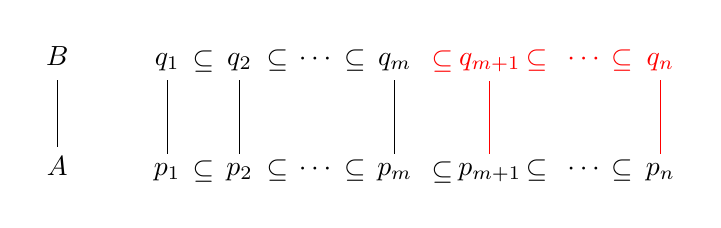
\begin{tikzpicture}[
      compare/.code n args={4}{%
        \ifnum#1>#2
          \pgfkeysalso{#3}
        \else
          \pgfkeysalso{#4}
        \fi
      }
    ]
      \matrix (M) [matrix of math nodes,row sep=2.4em,column sep=1em]
      {
        B\vphantom{\ideal q_1} &[5mm] \ideal q_1 & \ideal q_2 & \cdots & \ideal q_m & |[red]|\ideal q_{m+1} &
        |[red]|\cdots & |[red]|\ideal q_n \\
        A & \ideal p_1 & \ideal p_2 & \cdots & \ideal p_m & \ideal p_{m+1} &
        \cdots & \ideal p_n \\
      };
      \foreach \i [evaluate=\i as \j using int(\i+1)] in {2,...,7}
      {
        \node [compare={\i}{4}{red}{black}] at ($(M-1-\i)!0.5!(M-1-\j)$) {$\subseteq$};
        \node at ($(M-2-\i)!0.5!(M-2-\j)$) {$\subseteq$};
        \ifnum\i=4
        \else
          \ifnum\i=7
          \else
            \draw [compare={\i}{5}{red}{black}] (M-1-\i) -- (M-2-\i);
          \fi
        \fi
      }
      \draw [red] (M-1-8) -- (M-2-8);
      \draw (M-1-1) -- (M-2-1);
    \end{tikzpicture}
    \caption{上行定理}\label{fig:going-up}
\end{figure}

\begin{proof}
  我们只需要证明存在 $\ideal q_{m+1}$
  使得 $\ideal q_{m+1}\cap A=\ideal p_{m+1}$ 即可。
  根据 \autoref{prop:quotient preserve integral dependence},$\bar B=B/\ideal q_{m}$
  在 $\bar A=A/\ideal p_m$ 上是整的,我们有交换图
  \[
    \begin{tikzcd}
      A\arrow[r,"j"]\arrow[d,"\pi_1"'] & B\arrow[d,"\pi_2"] \\
      \bar A\arrow[r,"\bar j"] & \bar B
    \end{tikzcd}  
  \]
  $\bar{\ideal p}_{m+1}$ 是 $\bar A$ 的素理想,
  根据 \autoref{thm:lying over},存在 $\bar B$ 的素理想 $\bar{\ideal q}_{m+1}$
  使得 $\bar j^{-1}(\bar{\ideal q}_{m+1})=\bar{\ideal p}_{m+1}$,
  $\bar{\ideal q}_{m+1}$ 对应到 $B$ 的素理想 $\ideal q_{m+1}$,此时
  \[
    \ideal q_{m+1}\cap A=j^{-1}(\ideal q_{m+1})
    =(\pi_2\circ j)^{-1}(\bar{\ideal q}_{m+1})=(\bar j\circ\pi_1)^{-1}(\bar{\ideal q}_{m+1})
    =\ideal p_{m+1}.\qedhere
  \]
\end{proof}

\section{整闭整环和下行定理}

\begin{proposition}\label{prop:integrally closed in fraction}
  令 $A\subseteq B$ 是环,$C$ 是 $A$ 在 $B$ 中的整闭包,令 $S$ 是 $A$ 的乘性子集,
  那么 $S^{-1}C$ 是 $S^{-1}A$ 在 $S^{-1}B$ 中的整闭包。
\end{proposition}
\begin{proof}
  根据 \autoref{prop:quotient preserve integral dependence},$S^{-1}C$ 在 $S^{-1}A$ 
  上是整的。任取 $b/s\in S^{-1}B$,若 $b/s$ 在 $S^{-1}A$ 上是整的,
  则 $b/s$ 满足某个 $S^{-1}A$ 为系数的方程
  \[
    (b/s)^n+(a_1/s_1)(b/s)^{n-1}+\cdots+(a_n/s_n)=0,  
  \]
  令 $t=s_1\cdots s_n$,两边同时乘以 $(st)^n/1$,那么
  \[
    (bt)^n/1+(a_1st/s_1)(bt)^{n-1}/1+\cdots+(a_ns^nt^n/s_n)=0,
  \]
  所以存在 $u\in S$ 使得
  \[
    u(bt)^n+ua_1' (bt)^{n-1}+\cdots+ua_n'=0,
  \] 
  两边同时乘以 $u^{n-1}$,那么
  \[
    (btu)^n+ua_1'(btu)^{n-1}  +\cdots+u^na_n'=0,
  \]
  这表明 $btu\in C$,所以 $b/s=btu/stu\in S^{-1}C$,所以 $S^{-1}C$ 是 $S^{-1}A$ 在 $S^{-1}B$ 中的整闭包。
\end{proof}

一个整环被称为\emph{整闭的},如果它在它的分式域中是整闭的。
例如,$\mathbb{Z}$ 是整闭的。

\begin{example}
  UFD 都是整闭的。设 $R$ 是 UFD,任取 $x/y\in \Frac(R)$,$y\neq 0$,
  利用唯一因子分解,可以假设 $x,y$ 互素。若 $x/y$ 在 $R$ 上是整的,
  那么 $x/y$ 满足
  \[
    (x/y)^n+r_1(x/y)^{n-1}+\cdots+r_n=0\quad (r_i\in R),
  \]
  两边乘以 $y^n$,那么
  \[
    x^n+r_1yx^{n-1}  +\cdots+r_ny^n=0,
  \]
  这表明 $y\mid x^n$,$x,y$ 互素表明 $y\in R^\times$,所以 $x/y=xy^{-1}/1\in R$,
  故 $R$ 在 $\Frac(R)$ 中整闭。
\end{example}

整闭是局部性质。

\begin{proposition}
  令 $A\subseteq B$ 是环,那么下面的说法是等价的:
  \begin{enumerate}
    \item $A$ 在 $B$ 中整闭;
    \item 对于每个素理想 $\ideal p\subseteq A$,$A_{\ideal p}$ 在 $B_{\ideal p}$
    中是整闭的;
    \item 对于每个极大理想 $\ideal m\subseteq A$,$A_{\ideal m}$ 在 $B_{\ideal m}$
    中是整闭的。
  \end{enumerate}
\end{proposition}
\begin{proof}
  $(1)\Rightarrow (2)$ \autoref{prop:integrally closed in fraction}。
  $(2)\Rightarrow (3)$ 极大理想都是素理想。

  $(3)\Rightarrow (1)$ 令 $C$ 为 $A$ 在 $B$ 中的整闭包,证明单位映射 $f:A\to C$ 是满射即可。
  根据 \autoref{prop:injective is local},等价于证明 $f_{\ideal m}:A_{\ideal m}\to C_{\ideal m}$
  是满射。根据 \autoref{prop:integrally closed in fraction},$C_{\ideal m}$ 是 $A_{\ideal m}$
  在 $B_{\ideal m}$ 中的整闭包,所以 $f_{\ideal m}$ 满射。
\end{proof}

\begin{corollary}
  令 $A$ 是整环,那么下面的说法是等价的:
  \begin{enumerate}
    \item $A$ 是整闭的;
    \item 对于每个素理想 $\ideal p\subseteq A$,$A_{\ideal p}$ 是整闭的;
    \item 对于每个极大理想 $\ideal m\subseteq A$,$A_{\ideal m}$ 是整闭的。
  \end{enumerate}
\end{corollary}

令 $A\subseteq B$ 是环,$\ideal a$ 是 $A$ 的理想。元素 $b\in B$ 如果满足
首一的以 $\ideal a$ 中元素为系数的多项式,那么我们说 $b$ \emph{在 $\ideal a$ 上是整的}。
$\ideal a$ \emph{在 $B$ 中的整闭包}指的是 $B$ 中所有在 $\ideal a$ 上整的元素的集合。

\begin{lemma}\label{lemma:closure of ideal}
  令 $C$ 是 $A$ 在 $B$ 中的整闭包,$\ideal aC$ 为 $\ideal a$ 在 $C$ 中的扩张。
  那么 $\ideal a$ 在 $B$ 中的整闭包是根式理想 $\sqrt{\ideal aC}$(从而对加减乘封闭)。
\end{lemma}
\begin{proof}
  若 $x\in B$ 在 $\ideal a$ 上是整的(自然在 $A$ 上也是整的),那么 $x$ 满足
  \[
    x^n+a_1x^{n-1}+\cdots+a_n=0\quad (a_i\in\ideal a),  
  \]
  所以 $x^n\in\ideal aC$,所以 $x\in\sqrt{\ideal aC}$。

  反过来,若 $x\in\sqrt{\ideal aC}$,那么存在 $n$ 使得 $x^n=\sum_{i=1}^m a_ic_i$,
  其中 $a_i\in\ideal a,c_i\in C$。因为 $c_1,\dots,c_m$ 在 $A$ 上是整的,
  所以 $M=A[c_1,\dots,c_m]$ 是有限生成 $A$-模。考虑 $\phi:M\to M$ 为
  $\phi(f(c_1,\dots,c_m))=x^nf(c_1,\dots,c_m)$,那么 $\phi$ 是 $A$-模同态,
  并且 $\phi(M)=x^nM\subseteq\ideal aM$,
  根据 Cayley-Hamilton 定理,存在 $a_i'\in \ideal a$ 使得
  \[
    \phi^k+a_1'\phi^{k-1}+\cdots+a_k'=0,  
  \]
  由于 $\phi(1)=x^n$,所以 
  \[
    x^{kn}+a_1'x^{(k-1)n}+\cdots+a_k'=0,
  \]
  即 $x$ 在 $\ideal a$ 上是整的。
\end{proof}

若 $A\subseteq B$ 是整环,$x\in B$ 在 $A$ 上是整的,$x$ 在 $\Frac(A)$ 上当然是代数的,
但是一般情况下,$x$ 在 $\Frac(A)$ 上的极小多项式不一定处于 $A[x]$ 中。例如,
记 $\omega=e^{2\pi i/3}$,$A=\mathbb{Z}[\sqrt{-3}]$,
$B=\mathbb{Z}[\omega]=\mathbb{Z}[\frac{1+\sqrt{-3}}{2}]$,$F=\Frac(A)=\mathbb{Q}(\sqrt{-3})$。
$\omega$ 在 $F$ 上的极小多项式显然为 $x-\omega$,但是 $\omega\notin A$。如果
$A$ 是整闭的,那么这个结论是正确的,即下面的命题。这个例子中,$B$
在 $A$ 上是整的,并且 $B$ 是 ED,从而是 UFD,从而是整闭的,所以 $A$ 在 $F$
中的整闭包是 $B$。

\begin{proposition}\label{prop:minimal polynominal of x}
  令 $A\subseteq B$ 是整环,$A$ 是整闭的,$x\in B$ 在 $A$ 的某个理想 $\ideal a$ 
  上是整的。那么 $x$ 在分式域 $K=\Frac(A)$ 上是代数的。此外,设 $x$ 在 $K$ 上的极小多项式
  为 $t^n+a_1t^{n-1}+\cdots+a_n$,那么 $a_1,\dots,a_n\in\sqrt{\ideal a}$。
\end{proposition}
\begin{proof}
  显然 $x$ 在 $K$ 上是代数的。记 $L$ 为 $f(t)=t^n+a_1t^{n-1}+\cdots+a_n$ 的分裂域,
  $f(t)$ 在 $L$ 上分裂为 $f(t)=(t-\alpha_1)\cdots(t-\alpha_n)$,不妨设 $\alpha_1=x$。
  那么我们有 $K(\alpha_i)\simeq K[t]/(f(t))\simeq K(x)$。
  设 $x$ 满足
  \[
    x^m+a_1'x^{m-1}+\cdots +a_m'=0\quad (a_i'\in \ideal a),  
  \]
  将上式放到 $L$ 中,由于 $K(\alpha_i)\simeq K(x)$,那么对于 $\alpha_i$,同样有 
  \[
    \alpha_i^m+a_1'\alpha_i^{m-1}+\cdots +a_m'=0,  
  \]
  所以 $\alpha_i$ 在 $\ideal a$ 上是整的。由 Vieta 定理,$a_i$ 可以表示为 $\alpha_1,\dots,\alpha_n$
  的对称多项式,考虑 $A\subseteq L$,根据 \autoref{lemma:closure of ideal},
  所以 $a_i$ 在 $\ideal a$ 上是整的(封闭性)。
  由于 $a_i\in K$,考虑 $A\subseteq K$,
  再根据 \autoref{lemma:closure of ideal},$a_i\in\sqrt{\ideal a^e}=\sqrt{\ideal a}$。
\end{proof}

\begin{theorem}[下行定理]
  令 $A\subseteq B$ 是整环,$A$ 是整闭的,$B$ 在 $A$ 上是整的。令 
  $\ideal p_1\supseteq \cdots\supseteq\ideal p_n$ 是 $A$ 的素理想链,
  $\ideal q_1\supseteq\cdots\supseteq \ideal q_m\ (m< n)$ 是 $B$ 的素理想链,
  并且 $\ideal q_i\cap A=\ideal p_i\ (1\leq i\leq m)$。那么 
  $\ideal q_1\supseteq\cdots\supseteq \ideal q_m$ 可以被扩张到链
  $\ideal q_1\supseteq\cdots\supseteq \ideal q_n$ 使得 $\ideal q_i\cap A=\ideal p_i\ (1\leq i\leq n)$。
  如 \autoref{fig:going-down} 所示。
\end{theorem}

\begin{figure}[htb]
  \centering
  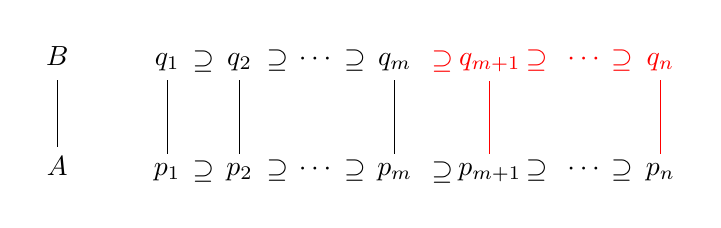
\begin{tikzpicture}[
    compare/.code n args={4}{%
      \ifnum#1>#2
        \pgfkeysalso{#3}
      \else
        \pgfkeysalso{#4}
      \fi
    }
  ]
    \matrix (M) [matrix of math nodes,row sep=2.4em,column sep=1em]
    {
      B\vphantom{\ideal q_1} &[5mm] \ideal q_1 & \ideal q_2 & \cdots & \ideal q_m & |[red]|\ideal q_{m+1} &
      |[red]|\cdots & |[red]|\ideal q_n \\
      A & \ideal p_1 & \ideal p_2 & \cdots & \ideal p_m & \ideal p_{m+1} &
      \cdots & \ideal p_n \\
    };
    \foreach \i [evaluate=\i as \j using int(\i+1)] in {2,...,7}
    {
      \node [compare={\i}{4}{red}{black}] at ($(M-1-\i)!0.5!(M-1-\j)$) {$\supseteq$};
      \node at ($(M-2-\i)!0.5!(M-2-\j)$) {$\supseteq$};
      \ifnum\i=4
      \else
        \ifnum\i=7
        \else
          \draw [compare={\i}{5}{red}{black}] (M-1-\i) -- (M-2-\i);
        \fi
      \fi
    }
    \draw [red] (M-1-8) -- (M-2-8);
    \draw (M-1-1) -- (M-2-1);
  \end{tikzpicture}
  \caption{下行定理}\label{fig:going-down}
\end{figure}

\begin{proof}
  我们只需要证明存在 $\ideal q_{m+1}\subseteq\ideal q_m$ 使得 $\ideal q_{m+1}\cap A=\ideal p_{m+1}$ 即可,
  我们有交换图
  \[
    \begin{tikzcd}
      A\arrow[r,"j"]\arrow[d,"\alpha"'] & B\arrow[d,"\beta"]\\
      A_{\ideal p_{m}}\arrow[r,"j'"] & B_{\ideal q_{m}}
    \end{tikzcd}  
  \]
  注意由于 $A-\ideal p_{m}\subseteq B-\ideal q_m$,所以 $A_{\ideal p_m}\to B_{\ideal q_m}$
  的映射是良定义的。考虑 $\beta\circ j:A\to B_{\ideal q_m}$,注意 $A,B$
  是整环表明 $\alpha,\beta$ 是单射。由于 $B$ 的被 $\ideal q_m$ 包含的素理想一一
  对应到 $B_{\ideal q_m}$ 的素理想,
  所以等价于证明 $\ideal p_{m+1}$ 是 $B_{\ideal q_m}$ 的某个素理想的收缩。根据
  \autoref{prop:condition of contraction},等价于证明
  $\bigl(\ideal p_{m+1}B_{\ideal q_m}\bigr)\cap A=\ideal p_{m+1}$(由于 $\beta\circ j$
  是单射,所以可以将 $A$ 视为 $B_{\ideal q_m}$ 的子环)。
  由于我们总是有 $\bigl(\ideal p_{m+1}B_{\ideal q_m}\bigr)\cap A\supseteq \ideal p_{m+1}$,
  所以只需要证明 $\bigl(\ideal p_{m+1}B_{\ideal q_m}\bigr)\cap A\subseteq\ideal p_{m+1}$。

  任取 $y/s\in\bigl(\ideal p_{m+1}B_{\ideal q_m}\bigr)\cap A$,其中 $y\in \ideal p_{m+1}B$,
  $s\in B-\ideal q_m$,根据 \autoref{lemma:closure of ideal},所以 $y$ 在 $\ideal p_{m+1}$
  上是整的。根据 \autoref{prop:minimal polynominal of x},$y$ 在 $\Frac(A)$ 上的极小多项式
  为
  \[
    y^n+u_1y^{n-1}+\cdots+u_n=0\quad (u_i\in\sqrt{\ideal p_{m+1}}=\ideal p_{m+1}).  
  \]

  $y/s\in A$ 说明存在 $x\in A$ 使得 $y/s=x/1$,即存在 $t\in B-\ideal q_m$ 使得
  $t(y-sx)=0$,$t\neq 0$ 表明 $y=sx$,那么在 $\Frac(B)\supseteq \Frac(A)$ 中有 $s=yx^{-1}$。
  那么 $s$ 在 $\Frac(A)$ 上的极小多项式为
  \[
    s^n+v_1s^{n-1}+\cdots+s_n=0,  
  \]
  其中 $v_i=u_i/x^i$。所以,我们有 $x^iv_i=u_i\in\ideal p_{m+1}$。

  因为 $s$ 在 $A$ 上是整的,根据 \autoref{prop:minimal polynominal of x},
  所以 $s$ 在 $\Frac(A)$ 上的极小多项式的系数在 $A$ 中,即 $v_i\in A$。
  假设 $x\notin \ideal p_{m+1}$,那么 $x^iv_i\in\ideal p_{m+1}$ 表明 $v_i\in\ideal p_{m+1}$,
  所以 $s^n\in\ideal p_{m+1}B\subseteq \ideal p_mB\subseteq \ideal q_m$,所以 $s\in\ideal q_m$,
  矛盾。故 $x\in\ideal p_{m+1}$,即 $\bigl(\ideal p_{m+1}B_{\ideal q_m}\bigr)\cap A\subseteq\ideal p_{m+1}$。
\end{proof}

下面我们简要回顾双线性型的一些内容。令 $V$ 是有限维 $F$-向量空间,$B:V\times V\to F$
是一个双线性型($F$-双线性映射)。用张量积的性质来说,$B$ 对应一个 $V\otimes_F V\to F$
的线性映射,即 $B\in (V\otimes_F V)^*$。$B$ 诱导出两个 $V\to V^*$ 的线性映射,即
\[
  B_l:x\mapsto (B(x,\uline{}):y\mapsto B(x,y)) ,\quad
  B_r:x\mapsto (B(\uline{},x):y\mapsto B(y,x)) .
\]
如果上述两个线性映射是单射,那么我们说 $B$ 是\emph{非退化的}。
由于 $\dim V=\dim V^*$,所以 $B$ 是非退化的当且仅当 $B_l$ 和 $B_r$
是同构。设 $V$ 的一组基为 $e_1,\dots,e_n$。记矩阵 $\mathbold B=\bigl(B(e_i,e_j)\bigr)_{n\times n}$,
对于 $u,v\in V$,设 $u=u_1e_1+\cdots+u_ne_n$ 以及 $v=v_1e_1+\cdots+v_ne_n$,
那么
\[
  B(u,v)=B\left(\sum_i u_ie_i,\sum_j v_je_j\right)  =
  \sum_i\sum_j u_iv_jB(e_i,e_j)=\mathbold u^\top\mathbold B\mathbold v,
\]
其中 $\mathbold u=(u_1,\dots,u_n)$ 以及 $\mathbold v=(v_1,\dots,v_n)$。
不难证明 $B$ 非退化当且仅当 $\mathbold B$ 可逆。

现在假设 $B$ 是对称双线性型。如果 $B$ 非退化,那么 $B_l:V\to V^*$
是同构。设 $V$ 的一组基为 $e_1,\dots,e_n$,那么 $V^*$ 的基为 $e_1^*,\dots,e_n^*$,满足
$e_i^*(e_j)=\delta_{ij}$。于是存在基 $v_1,\dots,v_n\in V$ 使得 $B(v_i,\uline)=e_i^*$,
即 $B(v_i,e_j)=\delta_{ij}$。

然后我们简要介绍一下关于域扩张中迹的概念。令 $K/F$ 是有限扩张,$[K:F]=n$。对于 $a\in K$,
定义映射 $L_a:K\to K$ 为 $L_a(x)=ax$。容易验证 $L_a$ 为 $F$-线性映射,那么我们可以定义
元素 $a$ 的迹为线性映射 $L_a$ 的迹,即
\[
  \Tr_{K/F}(a)=\Tr(L_a).  
\]
这诱导了 $F$-线性映射 $\Tr_{K/F}:K\to F$。当 $c\in F$ 的时候,设 $K$ 的一组基
为 $v_1,\dots,v_n$,那么 $L_c$ 在这组基下的表示矩阵为 $cI_n$,所以
$\Tr_{K/F}(c)=cn$。

$\Tr_{K/F}$ 也诱导了一个 $F$-双线性映射 $\Tr_{K/F}:K\times K\to F$,即
$\Tr_{K/F}(a,b)=\Tr_{K/F}(ab)$。容易验证 $\Tr_{K/F}$ 是对称双线性型。
我们不加证明地给出结论:$K/F$ 是可分扩张当且仅当 $\Tr_{K/F}$ 是非退化的。

\begin{proposition}\label{prop:basis of integral closure}
  $A$ 是任意整闭整环,$K$ 是 $A$ 的分式域,$L$ 是 $K$ 的有限可分扩张,$B$ 是 $A$ 
  在 $L$ 中的整闭包。那么存在 $K$-向量空间 $L$ 的一组基 $v_1,\dots,v_n$
  使得 $B\subseteq \sum_{j=1}^n Av_j$。
\end{proposition}
\begin{proof}
  设 $[L:K]=n$。首先我们断言:存在 $L$ 的一组基 $u_1,\dots,u_n$ 使得 $u_i\in B$。
  任取 $L$ 的一组基 $u_1',\dots,u_n'$,那么 $u_i'$ 在 $K$ 上是代数的,所以满足方程
  (总是可以乘以公分母使得系数处于 $A$ 中)
  \[
    a_m(u_i')^m+a_{m-1}(u_i')^{m-1}+\cdots+  a_0=0\quad (a_m\neq 0, a_j\in A).
  \]
  两边乘以 $a_m^{m-1}$,所以
  \[
    (a_mu_i')^m+a_{m-1}a_m(a_mu_i')^{m-1}+\cdots+a_0 a_m^{m-1}=0,  
  \]
  令 $u_i=a_mu_i'$,那么 $u_i$ 在 $A$ 上是整的,并且仍然是 $L$ 的一组基。

  根据上面的叙述,$L/K$ 可分表明 $\Tr_{L/K}$ 是非退化的,所以存在 $L$ 的一组基 $v_1,\dots,v_n$
  使得 $\Tr_{L/K}(u_iv_j)=\delta_{ij}$。任取 $x\in B$,设 $x=\sum_j x_jv_j$,其中 $x_j\in K$,
  那么
  \[
    x_j=\sum_i\delta_{ji}x_i=\sum_i\Tr_{L/K}(u_jv_i)x_i
    =\Tr_{L/K}(xu_j),
  \]
  所以 $x=\sum_j \Tr_{L/K}(xu_j)v_j$。下面我们说明,对于任意的 $y\in B$,都有
  $\Tr_{L/K}(y)\in A$ 即可。由于
  \begin{align*}
    \Tr_{L/K}(y)&=\Tr_{K(y)/K}\circ \Tr_{L/K(y)}(y)=\Tr_{K(y)/K}\bigl([L:K(y)]\cdot y\bigr)\\
    &=[L:K(y)]\cdot \Tr_{K(y)/K}(y).
  \end{align*}
  设 $[K(y):K]=m$,那么 $K(y)$ 的一组基为 $1,y,\dots,y^{m-1}$。设 $y$ 在 $K$
  上的极小多项式为
  \[
    y^m+a_{m-1}  y^{m-1}+\cdots+a_0=0,
  \]
  根据 \autoref{prop:minimal polynominal of x},$a_i\in A$。线性映射 $L_y:K(y)\to K(y)$
  在上述基下的表示矩阵为
  \[
    \begin{pmatrix*}
      0 & & & & -a_0\\
      1 & 0 & && -a_1\\
      & 1 & \ddots & & \vdots\\
      & & \ddots& 0 &-a_{m-1}\\
      & & & 1 & -a_m\\
    \end{pmatrix*}  ,
  \]
  所以 $\Tr_{L/K}(y)=[L:K(y)]\cdot (-a_{m})\in A$。
\end{proof}

\section{赋值环}

$K$ 是一个域,$K$ 的一个\emph{离散赋值}指的是一个映射 $v:K^\times\to\mathbb{Z}$,
其满足
\begin{enumerate}
  \item $v(xy)=v(x)+v(y)$,即 $v$ 是群同态;
  \item $v(x+y)\geq\min(v(x),v(y))$。
\end{enumerate}
为了方便起见,定义 $v(0)=+\infty$。容易观察到这蕴含着 $v(1)=v(-1)=0$ 以及
$v(x)=v(-x)$。

\begin{example}
  \mbox{}
  \begin{enumerate}
    \item 固定素数 $p\in\mathbb{Z}$,任意的 $x\in\mathbb{Q}^\times$ 可以唯一地写为
    $x=p^r\frac{a}{b}$,其中 $a,b$ 互素并且 $p\nmid a$ 以及 $p\nmid b$。定义
    $v_p:\mathbb{Q}^\times \to\mathbb{Z}$ 为 $v_p(x)=r$。
    对于 $x=p^r\frac{a}{b}$ 以及 $y=p^s\frac{c}{d}$,有 $xy=p^{r+s}\frac{ac}{bd}$,
    此时 $p\nmid ac$ 以及 $p\nmid bd$,所以 $v_p(xy)=r+s=v_p(x)+v_p(y)$。
    不妨设 $r\leq s$,我们有
    \[
      x+y=p^r\left(\frac{a}{b}+p^{s-r}\frac{c}{d}\right)=p^r\frac{ad+p^{s-r}bc}{bd}  ,
    \]
    此时 $p\nmid bd$,当 $r<s$ 时有 $p\nmid (ad+p^{s-r}bc)$,此时 $v_p(x+y)=r$。
    当 $r=s$ 时 $ad+bc$ 可能含有 $p$ 作为因子,此时 $v_p(x+y)\geq r$。所以
    $v_p$ 是 $\mathbb{Q}$ 的离散赋值。
  \end{enumerate}
\end{example}

\begin{lemma}
  $K$ 是一个域,有离散赋值 $v:K^\times\to\mathbb{Z}$,若 $v(x)\neq v(y)$,那么
  $v(x+y)=\min(v(x),v(y))$。
\end{lemma}
\begin{proof}
  不妨设 $v(x)>v(y)$,那么 $v(x+y)\geq \min(v(x),v(y))=v(y)$。
  另一方面,我们有
  \[
    v(y)=v(x+y-x)\geq \min(v(x+y),v(-x))=  \min(v(x+y),v(x)),
  \]
  若 $v(x)\leq v(x+y)$,那么 $v(y)\geq v(x)$,与 $v(x)>v(y)$ 矛盾。所以只可能
  $v(x)>v(x+y)$,故 $v(y)\geq v(x+y)$。所以 $v(x+y)=v(y)=\min(v(x),v(y))$。
\end{proof}

\begin{proposition}
  $K$ 是一个域,有离散赋值 $v:K^\times\to\mathbb{Z}$,定义
  \[
    A=\{x\in K\,|\, v(x)\geq 0\},\quad \ideal m=\{x\in K\,|\, v(x)>0\},
  \]
  那么 
  \begin{enumerate}
    \item $A$ 是 $K$ 的一个子环,并且对于任意的 $x\in K^\times$,有 $x\in A$ 或者
    $x^{-1}\in A$(或者均有)。
    \item $\ideal m$ 是 $A$ 的唯一的极大理想。
  \end{enumerate}
\end{proposition}
\begin{proof}
  (1) $v$ 是群同态表明 $v(1)=0$,故 $1\in A$。任取 $x,y\in A$,
  那么 $v(x-y)\geq \min (v(x),v(-y))=\min(v(x),v(y))\geq 0$,
  所以 $x-y\in A$。此外,$v(xy)=v(x)+v(y)\geq 0$,所以 $xy\in A$。这就表明 $A$ 是
  $K$ 的子环。任取 $x\in K^\times$,如果 $x\notin A$,那么 $v(x)<0$,那么 $0=v(1)=v(x)+v(x^{-1})$,
  故 $v(x^{-1})>0$,所以 $x^{-1}\in A$,所以必有 $x\in A$ 或者 $x^{-1}\in A$。

  (2) 任取 $x\in\ideal m$,$a\in A$,那么 $v(ax)=v(a)+v(x)>0$,所以 $ax\in\ideal m$。
  任取 $x,y\in\ideal m$,那么 $v(x-y)\geq \min(v(x),v(y))>0$,所以 $x-y\in\ideal m$。
  这表明 $\ideal m$ 是 $A$ 的一个理想。任取 $x\in A-\ideal m$,那么
  $v(x)=0$,所以 $0=v(1)=v(x)+v(x^{-1})$ 表明 $v(x^{-1})=0$,故 $x^{-1}\in A$,
  所以 $x\in A^\times$。这就表明 $A-\ideal m=A^\times$,所以 $\ideal m$ 是 $A$
  唯一的极大理想,$A$ 是局部环。
\end{proof}

令 $B$ 是整环,$K$ 是 $B$ 的分式域,如果对于 $x\neq 0$,总是有 $x\in B$ 或者 $x^{-1}\in B$(或者都有),
那么称 $B$ 是 $K$ 的\emph{赋值环}。反之,如果 $K$ 的子环 $B$ 满足
对于 $x\neq 0$,总是有 $x\in B$ 或者 $x^{-1}\in B$,那么 $x=1/x^{-1}\in\Frac(B)$,所以
此时 $K$ 就是 $B$ 的分式域,即 $B$ 是 $K$ 的赋值环。

\begin{proposition}
  \mbox{}
  \begin{enumerate}
    \item $B$ 是局部环。
    \item 如果 $B'$ 是环使得 $B\subseteq B'\subseteq K$,那么 $B'$ 也是 $K$ 的赋值环。
    \item $B$ 是整闭的(在 $K$ 中)。
  \end{enumerate}
\end{proposition}
\begin{proof}
  令 $\ideal m$ 为 $B$ 中所有不是单位的元素的集合。若 $x\in\ideal m$,$b\in B$,
  那么 $x^{-1}\notin B$,所以 $(bx)^{-1}=b^{-1}x^{-1}\notin B$,这就表明一定有
  $bx\in B$ 且 $bx$ 在 $B$ 中不可逆,故 $bx\in\ideal m$。
  若 $x,y\in\ideal m$,那么 $xy^{-1}\in B$ 或者 $x^{-1}y\in B$,所以
  $x-y=x(1-x^{-1}y)=y(xy^{-1}-1)\in \ideal m$。这表明 $\ideal m$ 是理想,而
  $B-\ideal m=B^\times$,所以 $\ideal m$ 是 $B$ 的唯一的极大理想。

  (2) 显然。

  (3) 令 $x\in K$ 在 $B$ 上是整的。那么 $x$ 满足方程
  \[
    x^n+b_1x^{n-1}+\cdots+b_n=0\quad (b_i\in B).  
  \]
  如果 $x^{-1}\in B$,两边乘以 $x^{1-n}$,那么
  \[
    x=-(b_1+b_2x^{-1}+\cdots+b_nx^{1-n}) \in B. 
  \]
  如果 $x^{-1}\notin B$,根据定义必有 $x\in B$。所以总是有 $x\in B$,
  即 $B$ 是整闭的。
\end{proof}

\begin{proposition}
  $B$ 是域 $K$ 的赋值环当且仅当存在 $K$ 的离散赋值 $v:K^\times\to \mathbb{Z}$,
  使得
  \[
    B=\{x\in K\,|\, v(x)\geq 0\}  .
  \]
\end{proposition}

对于两个局部环 $(A,\ideal m)$ 和 $(B,\ideal n)$,我们说 $B$ 控制 $A$ 当且仅当
$A\subseteq B$ 并且 $\ideal m\subseteq\ideal n$。

\begin{theorem}\label{thm:existence of valuation ring}
  令 $K$ 是一个域,$A\subseteq K$ 是子环,$\ideal p$ 是 $A$ 的素理想,$\Omega$
  是包含剩余域 $k(\ideal p)$ 的代数闭域,那么存在 $K$ 的一个赋值环 $(B,\ideal m)$
  并且其控制 $(A_{\ideal p},\ideal pA_{\ideal p})$,此外,存在环同态 $g:B\to\Omega$
  使得 $\ker g=\ideal m$。
\end{theorem}
\begin{remark}
  若取 $\Omega$ 为 $k(\ideal p)$ 的代数闭包,该定理的含义为如下交换图:
  \[
    \begin{tikzcd}[row sep=2.4em]
      A\arrow[r] & A_{\ideal p}\arrow[r]\arrow[d,dashed,hookrightarrow,red] 
      & k(\ideal p)\arrow[r,hookrightarrow] \arrow[d,dashed,hookrightarrow,red] 
      & \overline{k(\ideal p)} \\
      & |[red]|B\arrow[r,red] & |[red]|B/\ideal m\arrow[ur,dashed,hookrightarrow,red]  & 
    \end{tikzcd}  
  \]
  也就是说:令 $K$ 是一个域,$A\subseteq K$ 是子环,$\ideal p$ 是 $A$ 的素理想,
  那么存在 $K$ 的一个赋值环 $(B,\ideal m)$ 并且其控制 $(A_{\ideal p},\ideal pA_{\ideal p})$,
  此外,$B/\ideal m$ 是 $k(\ideal p)$ 的代数扩张。
\end{remark}
\begin{proof}
  对于环 $A$,诱导出映射 $f:A\to A_{\ideal p}\to k(\ideal p)\hookrightarrow\Omega$。
  记集合 $\Sigma$ 是二元组 $(A',f')$ 的集合,其中 $A'$ 是满足 $A\subseteq A'\subseteq K$
  的子环,映射 $f':A'\to\Omega$ 满足 $f'|_A=f$。首先 $(A,f)\in\Omega$,所以 $\Omega\neq\emptyset$。
  定义 $\Omega$ 上的偏序:$(A',f')\leq (A'',f'')$ 当且仅当 $A'\subseteq A''$ 以及 $f''|_{A'}=f'$。

  上述偏序的含义如下:记 $\ideal p'=\ker f'$,由于 $f':A'\to\Omega$ 表明 $A'/\ideal p'$
  同构于 $\Omega$ 的子环是整环,所以 $\ideal p'$ 是素理想。类似地,记素理想 $\ideal p''=\ker f''$。
  那么 $f''|_{A'}=f'$ 表明 $\ideal p''\cap A'=\ideal p'$,即对于 $A'\hookrightarrow A''$ 有
  $\ideal p''^{c}=\ideal p'$。也就是说我们有如下交换图:
  \[
    \begin{tikzcd}[row sep=2.4em]
      A'\arrow[r]\arrow[d,hookrightarrow]
      & A'/\ideal p'\arrow[r]\arrow[d,hookrightarrow] 
      & k(\ideal p')\arrow[r,hookrightarrow]\arrow[d,hookrightarrow] 
      & \Omega \\
      A''\arrow[r] & A''/\ideal p''\arrow[r] & k(\ideal p'')\arrow[ur,hookrightarrow] & 
    \end{tikzcd}  
  \]

  令 $\{(A_i,f_i)\}_{i\in I}$ 是 $\Sigma$ 的一条链。令 $A_0=\bigcup_{i\in I}A_i$,对于 $x\in A_0$,
  那么存在 $i\in I$ 使得 $x\in A_i$,定义 $f_0:A_0\to\Omega$ 为 $f_0(x)=f_i(x)$。$f_0$
  是良定义的,因为若同时有 $x\in A_i$ 以及 $x\in A_j$,设 $(A_i,f_i)\leq (A_j,f_j)$,那么
  $f_i(x)=f_j(x)$。此时 $(A_0,f_0)$ 为这条链的上界,根据 Zorn 引理,$\Sigma$ 有极大元,
  记为 $(B,g)$。下面我们分三步证明 $B$ 就是我们要找的赋值环。

  Step 1. 证明 $B$ 是局部环,有极大理想 $\ideal m=\ker g$。首先 $\ideal m$ 是素理想,
  并且 $g(B-\ideal m)\neq 0$,所以 $g(B-\ideal m)\in\Omega^\times$,根据分式环的泛性质
  \ref{prop:universal property of fraction ring},存在交换图
  \[
    \begin{tikzcd}
      B\arrow[r,"g"]\arrow[d] & \Omega \\
      B_{\ideal m}\arrow[ur,dashed,"g'"'] &
    \end{tikzcd}  
  \]
  $B$ 是整环,所以 $B\to B_{\ideal m}$ 是单射,所以 $(B,g)\leq (B_{\ideal m},g')$,
  $(B,g)$ 是极大元表明 $B=B_{\ideal m}$。

  Step 2. 证明若 $x\notin B$,则 $\ideal mB[x]=B[x]$。这里 $B[x]$ 是 $K$ 中同时包含 $B$
  和 $x$ 的最小的子环。反证法,假设 $\ideal mB[x]\neq B[x]$,那么存在 $B[x]$ 的极大理想 $\ideal m'$
  包含 $\ideal mB[x]$,那么对于 $B\hookrightarrow B[x]$ 有 $\ideal m\subseteq\ideal m'\cap B$,
  同时注意到 $\ideal m'\cap B\neq B$,所以 $\ideal m$ 是 $B$ 的极大理想表明 $\ideal m'\cap B=\ideal m$。
  于是我们有如下交换图:
  \[
    \begin{tikzcd}[row sep=2.4em]
      B\arrow[r]\arrow[d,hookrightarrow] 
      & B/\ideal m\arrow[r,hookrightarrow]\arrow[d,hookrightarrow] 
      & \Omega \\
      B[x]\arrow[r]\arrow[urr,dashed,red,bend right=60,"g'"'] 
      & B[x]/\ideal m'\arrow[ur,dashed,hookrightarrow] &
    \end{tikzcd}  
  \]
  \vskip-10pt \noindent
  也就是说,通过 $b+\ideal m\mapsto b+\ideal m'$,$B/\ideal m$ 可以视为
  $B[x]/\ideal m'$ 的子域。注意到 $B[x]/\ideal m'$ 的元素都可以写为
  $h(x)+\ideal m'=\bar h(\bar x)=\bar h(x+\ideal m')$ 的形式(其中 $h\in B[t],\bar h\in B/\ideal m[t]$),
  所以 $B[x]/\ideal m'$ 可以视为 $B/\ideal m[\bar x]$,而 $B/\ideal m[\bar x]$ 是域,所以
  $\bar x$ 在 $B/\ideal m$ 上是代数的,那么就存在嵌入 $B[x]/\ideal m'\hookrightarrow\Omega$。
  那么可以令 $g':B[x]\to\Omega$ 为上述交换图中的复合映射 $B[x]\to B[x]/\ideal m'\to\Omega$,
  此时有 $(B,g)\leq (B[x],g')$,所以 $B=B[x]$,这与 $x\notin B$ 矛盾。这就证明了 $\ideal mB[x]=B[x]$。

  Step 3. 证明 $B$ 是 $K$ 的赋值环。若 $x\notin B$,那么 $\ideal mB[x]=B[x]$,所以存在
  $u_i\in\ideal m$ 使得
  \[
    u_0+u_1x+\cdots+u_nx^n=1,  
  \]
  即 $1-u_0-u_1x-\cdots-u_nx^n=0$,因为 $1-u_0\in B-\ideal m=B^\times$,所以
  \[
    x^{-n}-(1-u_0)^{-1}u_1x^{1-n}-\cdots-(1-u_0)^{-1}u_n=0, 
  \]
  所以 $x^{-1}$ 在 $B$ 上是整的,$B[x^{-1}]$ 在 $B$ 上是整的。根据 \autoref{thm:lying over},
  存在 $B[x^{-1}]$ 的素理想 $\ideal m'$ 使得 $\ideal m'\cap B=\ideal m$。实际上 $\ideal m'$
  必为极大理想,否则存在 $B[x^{-1}]$ 的极大理想 $\ideal n'$ 使得 $\ideal m'\subseteq\ideal n'$,
  于是 $\ideal m=\ideal m'\cap B\subseteq\ideal n'\cap B$,那么 $\ideal n'\cap B=\ideal m$,
  根据 \autoref{coro:contraction of prime ideal},有 $\ideal m'=\ideal n'$。再重复上面的叙述,
  我们可以得到 $g':B[x^{-1}]\to\Omega$ 使得 $(B,g)\leq (B[x^{-1}],g')$,所以 $B[x^{-1}]=B$,
  故 $x^{-1}\in B$,所以 $B$ 是 $K$ 的赋值环。此外,$(B,g)\in\Sigma$ 就表明
  $A\subseteq B$ 以及 $\ideal pA_{\ideal p}\subseteq\ideal m=\ker g$。
\end{proof}

\begin{corollary}\label{coro:integral closure is intersection of valuation ring}
  令 $A$ 是域 $K$ 的子环,那么 $A$ 在 $K$ 中的整闭包 $\bar A$ 是 $K$ 的所有包含 $A$
  的赋值环的交。
\end{corollary}
\begin{proof}
  令 $B$ 是 $K$ 的赋值环且 $A\subseteq B$。因为 $B$ 是整闭的,所以 $\bar A\subseteq B$。
  故 $\bar A$ 被 $K$ 的所有包含 $A$ 的赋值环的交包含。

  反之,令 $x\notin\bar A$,那么 $x\notin A[x^{-1}]=A'$,否则存在 $a_0,\dots,a_n\in A$
  使得
  \[
    x=a_0+ a_1x^{-1}+\cdots+a_nx^{-n},
  \]
  即 $x^{n+1}-a_0x^n-a_1x^{n-1}-\cdots-a_n=0$,这与 $x\notin\bar A$ 矛盾。所以 $x^{-1}$
  在 $A'$ 中不可逆,因此存在 $A'$ 的极大理想 $\ideal m'$ 使得 $x^{-1}\in\ideal m'$。
  那么存在 $K$ 的赋值环 $(B,\ideal m)$ 控制 $(A',\ideal m')$,注意 $\ideal m$ 为 $B$
  中不可逆元的集合,所以 $x^{-1}\in A'\subseteq B$ 表明 $x\notin B$。
  
  综上,这就表明 $\bar A$ 是 $K$ 的所有包含 $A$ 的赋值环的交。
\end{proof}

\begin{proposition}
  令 $A\subseteq B$ 是整环,$B$ 是有限生成 $A$-代数。令 $v$ 是 $B$ 中的非零元,那么存在
  $A$ 中的非零元 $u$ 使得:任取代数闭域 $\Omega$,任意同态 $f:A\to\Omega$ 如果满足
  $f(u)\neq 0$,那么 $f$ 可以被延拓为同态 $g:B\to\Omega$ 使得 $g(v)\neq 0$。
\end{proposition}
\begin{remark}
  记 $\ideal p=\ker f$ 和 $\ideal q=\ker g$ 是素理想,那么
  $g|_A=f$ 表明 $\ideal q\cap A=\ideal p$,并且 $f$
  可以通过商环分解为 $f:A\to A/\ideal p\to\Omega$,$g$ 同理,所以此时有交换图
  \[
    \begin{tikzcd}
      A\arrow[r]\arrow[d,hookrightarrow] 
      & A/\ideal p\arrow[r]\arrow[d,hookrightarrow]  & \Omega \\
      B\arrow[r] & B/\ideal q\arrow[ur,dashed,red] &
    \end{tikzcd}  
  \]
\end{remark}
\begin{proof}
  对 $B$ 的生成元的个数归纳,只需要证明 $B=A[x]$ 的情况即可。

  若 $x$ 在 $A$ 上是超越的(即 $x$ 不是任何 $A$ 中系数多项式的根)。对于非零元 $v\in B$,
  存在 $a_0,\dots,a_n\in A$ 使得 $v=a_0x^n+a_1x^{n-1}+\cdots+a_n$,其中 $a_0\neq 0$。
  取 $u=a_0$。如果同态 $f:A\to\Omega$ 满足 $f(u)\neq 0$,考虑 $\Omega[t]$ 中的多项式
  $f(a_0)t^n+f(a_1)t^{n-1}+\cdots+f(a_n)$,$\Omega$ 为代数闭域表明 $\Omega$ 为无限域,
  所以一定存在 $\xi\in\Omega$ 使得 $f(a_0)\xi^n+f(a_1)\xi^{n-1}+\cdots+f(a_n)\neq 0$。
  定义 $g:B\to\Omega$ 满足 $g(x)=\xi$ 以及 $g|_A=f$,那么 $g(v)\neq 0$ 满足条件。

  若 $x$ 在 $A$ 上是代数的(即 $x$ 是某个 $A$ 中系数多项式的根)。
  那么 $v^{-1}\in \Frac(B)$ 也是 $A[x]$ 中多项式的根,所以我们有
  \begin{gather*}
    a_0x^m+a_1x^{m-1}+\cdots+a_m=0\quad (a_i\in A),\\
    a_0'v^{-n}+a_1'v^{1-n}+\cdots+a_n'=0\quad (a_j'\in A).
  \end{gather*}
  令 $u=a_0a_0'$,若 $f:A\to\Omega$ 满足 $f(u)\neq 0$,那么 $f$ 可以延拓为
  $f_1:A[u^{-1}]\to\Omega$,满足 $f_1(u^{-1})=f(u)^{-1}$。根据 \autoref{thm:existence of valuation ring},
  存在 $\Frac(B)$ 的赋值环 $C$ 使得 $C\supseteq A[u^{-1}]$ 以及同态 $h:C\to\Omega$ 满足 $h|_A=f_1$。
  由于 $a_0x^m+a_1x^{m-1}+\cdots+a_m=0$,所以 $ux^m+a_1a_0'x^{m-1}+\cdots+a_ma_0'=0$,所以
  在 $A[u^{-1}]$ 中有
  \[
    x^m+a_1a_0'u^{-1}x^{m-1}+\cdots+a_ma_0'u^{-1}=0,
  \]
  即 $x$ 在 $A[u^{-1}]$ 上是整的。根据 \autoref{coro:integral closure is intersection of valuation ring},
  $x\in C$,所以 $B\subseteq C$。特别地,有 $v\in C$。另一方面,可以证明 $v^{-1}\in\Frac(B)$
  在 $A[u^{-1}]$ 上也是整的,所以 $v^{-1}\in C$。故 $v\in C^\times$,所以 $h(v)\neq 0$。
  令 $g=h|_B$ 即满足要求。
\end{proof}

\begin{corollary}[Zariski 引理]\label{coro:Zariski lemma}
  令 $k$ 是域,$B$ 是有限生成 $k$-代数,如果 $B$ 是域,那么 $B$ 是 $k$
  的有限(代数)扩张。
\end{corollary}
\begin{proof}
  取 $A=k$,$v=1$,$\Omega=\bar k$,那么嵌入 $j:k\to\bar k$ 可以延拓为同态
  $g:B\to\bar k$,$g(1)\neq 0$ 表明 $g$ 是非零同态,$B$ 是域进而表明 $g$
  是单同态,所以 $B$ 是 $k$ 的代数扩张。
\end{proof}

\autoref{coro:Zariski lemma} 是 Hilbert 零点定理(Hilbert's Nullstellensatz)的一种形式。
后面我们会介绍另一种证明方法(\autoref{prop:Zariski lemma 2})。

\section{EXERCISES}

\begin{problem}
  令 $f:A\to B$ 是环的整同态(即 $B$ 在 $ f(A)$ 上是整的),证明 $f^*:\Spec(B)\to\Spec(A)$
  是闭映射。
\end{problem}
\begin{proof}
  
\end{proof}

\begin{problem}
  令 $A$ 是 $B$ 的子环,$C$ 是 $A$ 在 $B$ 中的整闭包,证明 $C[x]$ 是 $A[x]$
  在 $B[x]$ 中的整闭包。
\end{problem}
\begin{proof}
  
\end{proof}

\begin{problem}
  $A,B$ 是两个局部环,如果 $A$ 是 $B$ 的子环并且 $A$ 的极大理想 $\ideal m$
  被 $B$ 的极大理想 $\ideal n$ 包含(等价地说,$\ideal m=\ideal n\cap A$),
  那么称 $B$ \emph{控制} $A$。令 $K$ 是域,$\Sigma$ 是 $K$ 的局部子环的集合,
  控制构成了 $\Sigma$ 上的一个偏序,证明 $\Sigma$ 有极大元,并且 $A\in\Sigma$
  是极大元当且仅当 $A$ 是 $K$ 的赋值环。
\end{problem}

\begin{problem}
  $A$ 是整环,$K$ 是 $A$ 的分式域,证明下面的说法是等价的:
  \begin{enumerate}
    \item $A$ 是 $K$ 的赋值环;
    \item 如果 $\ideal a,\ideal b$ 是 $A$ 的两个理想,那么 $\ideal a\subseteq \ideal b$
    或者 $\ideal b\subseteq\ideal a$。
  \end{enumerate}
  由此推断出,如果 $A$ 是一个赋值环,$\ideal p$ 是 $A$ 的一个素理想,那么 $A_{\ideal p}$
  和 $A/\ideal p$ 都是它们分式域的赋值环。
\end{problem}
\begin{proof}
  若 $A$ 是 $K$ 的赋值环,令 $\ideal a,\ideal b$ 是 $A$ 的两个不相同的理想,
  假设 $\ideal a\not\subseteq \ideal b$,我们证明 $\ideal b\subseteq\ideal a$。
  任取 $b\in\ideal b$,$\ideal a\not\subseteq\ideal b$ 表明存在 $a\in\ideal a-\ideal b$。
  $A$ 是赋值环表明 $a^{-1}b$ 或者 $ab^{-1}$ 在 $A$ 中。
  若 $ab^{-1}\in A$,那么 $a=b(ab^{-1})\in\ideal b$,这与
  $a\notin\ideal b$ 矛盾,所以 $a^{-1}b\in A$,所以
  $b=a(a^{-1}b)\in\ideal a$,故 $\ideal b\subseteq \ideal a$。

  反过来,令 $x\in K^\times$,假设 $x\notin A$。设 $x=a/b$,其中 $a,b\neq 0$,
  那么 $(a)\subseteq (b)$ 或者 $(b)\subseteq (a)$,即 $b\mid a$ 或者 $a\mid b$,
  即存在非零的 $c\in A$ 使得 $a=bc$ 或者 $b=ac$,如果 $a=bc$,那么 $x=c/1\in A$,
  所以有 $b=ac$,所以 $x^{-1}=b/a=c/1\in A$,所以 $A$ 是赋值环。

  $A_{\ideal p}$ 的理想都形如 $\ideal a_{\ideal p}$,其中 $\ideal a$ 是 $A$ 的被 $\ideal p$ 包含的理想。
  所以若 $\ideal a_{\ideal p},\ideal b_{\ideal p}$ 是 $A_{\ideal p}$ 的两个理想,
  那么 $\ideal a$ 和 $\ideal b$ 是 $A$ 的两个理想,所以 $\ideal a\subseteq \ideal b$
  或者 $\ideal b\subseteq \ideal a$,所以 $\ideal a_{\ideal p}\subseteq\ideal b_{\ideal p}$
  或者 $\ideal b_{\ideal p}\subseteq \ideal a_{\ideal p}$,即 $A_{\ideal p}$
  是赋值环。$A/\ideal p$ 的理想都形如 $\ideal a/\ideal p$,其中 $\ideal a$ 是包含 $\ideal p$ 的理想。
  剩余的叙述同理。
\end{proof}

\begin{problem}
  $A$ 是域 $K$ 的赋值环,$A$ 的单位群 $A^\times$ 是 $K$ 的乘法群 $K^\times$ 的子群。
  
  令 $\Gamma=K^\times/A^\times$,如果 $\bar x,\bar y\in\Gamma$,定义 $\bar x\geq \bar y$
  为 $xy^{-1}\in A$。证明这定义了 $\Gamma$ 上的一个全序,并且与群结构相容
  (即 $\bar x\geq \bar y\Rightarrow \bar x\bar w\geq \bar y\bar w\ (\forall\bar w\in\Gamma)$)。
  换句话说,$\Gamma$ 是一个全序的交换群,被称为 $A$ 的\emph{值群}。

  令 $v:K^\times \to\Gamma$ 是自然同态,证明 $v(x+y)\geq\min(v(x),v(y))$。
\end{problem}
\begin{proof}
  若 $\bar x_1=\bar x_2$ 以及 $\bar y_1=\bar y_2$,那么 $x_1^{-1}x_2\in A^\times$ 以及
  $y_1^{-1}y_2\in A^\times$。如果 $\bar x_1\geq \bar y_1$,那么
  $x_1y_1^{-1}\in A$,所以
  \[
    x_2y_2^{-1}=(x_2x_1^{-1})(x_1y_1^{-1})(y_1y_2^{-1})\in A,
  \]
  所以 $\bar x_2\geq \bar y_2$,所以 $\geq$ 是良定义的。
  
  对于任意的 $\bar x\in\Gamma$,由于 $xx^{-1}=1\in A$,所以 $\bar x\geq \bar x$。
  若 $\bar x\geq\bar y$ 以及 $\bar y\geq \bar z$,那么 $xy^{-1}\in A$ 以及
  $yz^{-1}\in A$,所以 $xz^{-1}=(xy^{-1})(yz^{-1})\in A$,所以 $\bar x\geq\bar z$。
  若 $\bar x\geq\bar y$ 以及 $\bar y\geq \bar x$,那么 $xy^{-1}\in A$ 以及
  $yx^{-1}\in A$,所以 $y^{-1}x=xy^{-1}\in A^\times$,所以 $x A^\times=yA^\times$,
  即 $\bar x=\bar y$。这表明 $\geq$ 是 $\Gamma$ 上的一个偏序。
  任取 $\bar x,\bar y\in\Gamma$,$A$ 是赋值环表明 $xy^{-1}\in A$ 或者 $yx^{-1}\in A$,
  即 $x\geq y$ 或者 $y\geq x$,所以 $\geq$ 是 $\Gamma$ 上的一个全序。

  若 $\bar x\geq \bar y$,任取 $\bar w\in\Gamma$,那么 $xw(yw)^{-1}=xy^{-1}\in A$,即
  $\bar x\bar w\geq \bar y\bar w$,所以 $\ge$ 与群结构相容。

  不妨设 $v(x)\geq v(y)$,即 $xy^{-1}\in A$,那么 $(x+y)y^{-1}=xy^{-1}+1\in A$,所以
  $v(x+y)\geq v(y)=\min(v(x),v(y))$。
\end{proof}




\chapter{链条件}

\section{Noether 模和 Artin 模}

令 $\Sigma$ 是集合,有偏序 $\leq$。

\begin{proposition}\label{prop:maximal condition}
  下面的说法是等价的:
  \begin{enumerate}
    \item $\Sigma$ 中的每个上升序列 $x_1\leq x_2\leq\cdots$ 是稳定的(即存在 $n$ 使得 $x_n=x_{n+1}=\cdots$)。
    \item $\Sigma$ 的任意非空子集都有极大元。
  \end{enumerate}
\end{proposition}
\begin{proof}
  $(1)\Rightarrow (2)$ 设 $S\subseteq\Sigma$ 是非空子集,假设其没有极大元。
  任取 $x_1\in S$,那么存在 $x_2\in S$ 并且 $x_1\neq x_2$ 使得 $x_1\leq x_2$,
  否则 $x_1$ 就是 $S$ 的极大元。同理,存在 $x_3\in S$ 并且 $x_3\neq x_2$
  使得 $x_2\leq x_3$。那么我们得到非稳定的上升序列 $x_1\leq x_2\leq \cdots$,
  矛盾。

  $(2)\Rightarrow (1)$ 对于上式序列 $x_1\leq x_2\leq \cdots$,考虑集合
  $(x_i)_{i\geq 1}$,这个集合有极大元 $x_n$,但是在 $i\geq n$ 时有 $x_n\leq x_i$,
  所以只可能 $x_n=x_i$,所以 $x_1\leq x_2\leq \cdots$ 是稳定的。
\end{proof}

对于一个模 $M$ 来说,令 $\Sigma$ 是 $M$ 的子模的集合,上面有偏序 $\subseteq$。
那么 \autoref{prop:maximal condition} 中的 (1) 被称为\emph{升链条件},
简写为 a.c.c.。(2) 被称为\emph{极大条件}。一个模 $M$ 如果满足这两个等价条件,
那么我们说 $M$ 是\emph{Noether 模}。一个环 $A$ 作为 $A$-模如果是 Noether 模,
那么我们说 $A$ 是\emph{Noether 环}。如果 $\Sigma$ 上面有偏序 $\supseteq$,
那么 (1) 被称为\emph{降链条件},简写为 d.c.c.。(2) 被称为\emph{极小条件}。
一个模 $M$ 如果满足这两个等价条件,
那么我们说 $M$ 是\emph{Artin 模}。一个环 $A$ 作为 $A$-模如果是 Artin 模,
那么我们说 $A$ 是\emph{Artin 环}。

\begin{example} 下面我们列举一些满足或者不满足 a.c.c.\ 和 d.c.c.\ 的例子。
  \begin{enumerate}
    \item 有限交换群(作为 $\mathbb{Z}$-模)同时满足 a.c.c.\ 和 d.c.c.,
    这是显然的,因为其只有有限个元素。$k$ 是域,$V$ 是有限维 $k$-向量空间,
    那么 $V$ 也同时满足 a.c.c\ 和 d.c.c.,因为 $V$ 的子空间都是有限维的。
    \item 假设 $A$ 是 PID,那么 $A$-子模相当于 $A$ 的理想。 
    令 $(a_1)\subseteq (a_2)\subseteq \cdots$ 是理想的升链,那么容易验证
    $\bigcup_i(a_i)$ 仍然是 $A$ 的理想,所以 $\bigcup_i (a_i)=(a)$。
    那么存在 $(a_n)$ 使得 $a\in (a_n)$,所以 $(a)\subseteq (a_n)$,那么
    对于 $i\geq n$,有 $(a_n)\subseteq (a_i)\subseteq \bigcup_i(a_i)=(a)\subseteq (a_n)$,
    所以 $(a_i)=(a_n)$。故 $A$ 满足 a.c.c.,即 PID 都满足 a.c.c.。
    \item 假设 $A$ 是整环但是不是域,任取 $a\in A- A^\times$ 并且 $a\neq 0$,考虑
    $(a)\supseteq (a^2)\supseteq (a^3)\supseteq \cdots$,如果 $(a^n)=(a^{n+1})$,
    那么存在 $b\in A$ 使得 $a^n=a^{n+1}b=a^nab$,所以 $ab=1$,与 $a$ 不可逆矛盾。所以
    上述降链是不稳定的。这表明非域的整环不满足 d.c.c.。结合 (2),我们知道
    $\mathbb{Z}$ 和域上的多项式环 $k[x]$ 是 Noether 环但不是 Artin 环。
    \item 考虑 $\mathbb{Z}$-模
    \[
      G=\left\{\bar x\in\mathbb{Q}/\mathbb{Z}\,\middle\vert\, x=\frac{a}{p^n}
      ,a\in\mathbb{Z},p\nmid a\right\}=\mathbb{Z}[1/p]/\mathbb{Z},
    \]
    令 $G_n=\frac{1}{p^n}\mathbb{Z}/\mathbb{Z}$ 是 $G$ 的子群($\mathbb{Z}$-子模)。
    那么 $G_0\subseteq G_1\subseteq G_2\subseteq \cdots$ 是严格上升的子模序列,
    所以 $G$ 不满足 a.c.c.。下面我们说明 $G$ 满足 d.c.c.。我们说明 $G$ 的恰当子群必为有限群,
    从而满足 d.c.c.。设 $H$ 是 $G$ 的子群。对于任意 $h=a/p^n\in H$,显然 $h$ 的阶 $|h|=p^n$。
    令 $p^n=\max\{|h|\,|\, h\in H\}$,其中 $n$ 可以为无穷。若 $n$ 有限,
    任取 $\overline{a/p^m}\in H$,因为 $|\overline{a/p^m}|=p^m\leq p^n$,所以
    $m\leq n$,所以 $\overline{a/p^m}=\overline{ap^{n-m}/p^n}\in G_n$。所以 $\langle h\rangle\subseteq H\subseteq G_n$,其中 $|h|=p^n$。由于 $G_n$ 是 $p^n$ 阶循环群,$\langle h\rangle$ 也是 $p^n$
    阶循环群,所以 $H=G_n$。若 $n$ 无穷,也就是说对于任意的 $m>0$,存在 $h_m=c/p^{n_m}\in H$,使得
    $|h_m|=p^{n_m}>p^m$,那么对于 $\overline{a/p^m}\in G_m$,有 
    $\overline{a/p^m}=\overline{ap^{n_m-m}/p^{n_m}}=ap^{n_m-m}\cdot \overline{1/p^{n_m}}$,
    所以 $\langle \overline{1/p^{n_m}}\rangle\supseteq G_m$,所以 $H\supseteq \bigcup_{m=1}^{\infty} G_m=G$,
    即 $H=G$。这就说明了 $G$ 的恰当子群必为有限群。所以 $G$ 作为 $\mathbb{Z}$-模是 Artin 模,但不是
    Noether 模。
    \item 域上无穷多个未定元的多项式环 $k[x_1,x_2,\dots]$ 既不满足 a.c.c.\ 又不满足 d.c.c.。
    因为 $(x_1)\subset (x_1,x_2)\subset (x_1,x_2,x_3)\subset\cdots$ 是不稳定的理想升链,
    $(x_1)\supset (x_1^2)\supset (x_1^3)\supset\cdots$ 是不稳定的理想降链。
    \item 我们后面将会证明对于环来说,满足 d.c.c.\ 必须满足 a.c.c.,即 Artin 环必为 Noether 环。
    对于模来说,(4) 表明模可以满足 d.c.c.\ 但是不满足 a.c.c.。
  \end{enumerate}
\end{example}

\begin{proposition}\label{prop:equiv condition of Noether}
  $M$ 是 Noether $A$-模当且仅当 $M$ 的每个子模都是有限生成的。
\end{proposition}
\begin{proof}
  若 $M$ 是 Noether $A$-模。设 $N$ 是 $M$ 的子模。令 $\Sigma$ 是 $N$ 的所有有限生成的子模
  的集合。由于 $(0)\in \Sigma$,所以 $\Sigma$ 非空。由于 $\Sigma$ 也是 $M$ 的有限生成子模的集合,
  所以存在极大元 $N'=(x_1,\dots,x_n)$。如果 $N'\neq N$,取 $x\in N-N'$,那么 $N'+(x)=(x_1,\dots,x_n,x)$
  是 $N$ 的有限生成子模,所以 $N'+(x)\in\Sigma$,但是 $N'+(x)\neq N'$,与 $N'$ 极大矛盾。所以
  $N=N'$ 是有限生成的。

  若 $M$ 的每个子模都是有限生成的。设 $N_1\subseteq N_2\subseteq \cdots$ 是 $M$ 的子模序列,
  令 $N=\bigcup_{i=1}^\infty N_i$。容易验证 $N$ 是 $M$ 的子模,所以是有限生成的。
  设 $N=(x_1,\dots,x_n)$。那么存在足够大的 $n$ 使得 $x_1,\dots,x_n\in N_n$,所以
  $N\subseteq N_n\subseteq N$,所以 $N_n=N$,于是 $i\geq n$ 时有 $N_i=N$。
  故 $M$ 满足 a.c.c.,即 $M$ 是 Noether 模。
\end{proof}
  
\begin{proposition}\label{prop:Noether of exact sequence}
  令
  $
    \begin{tikzcd}[cramped,column sep=small]
      0\arrow[r] & M'\arrow[r,"\alpha"] & M\arrow[r,"\beta"] & M''\arrow[r] & 0
    \end{tikzcd}
  $
  是 $A$-模的正合列,那么
  \begin{enumerate}
    \item $M$ 是 Noether 模当且仅当 $M'$ 和 $M''$ 是 Noether 模。
    \item $M$ 是 Artin 模当且仅当 $M'$ 和 $M''$ 是 Artin 模。
  \end{enumerate}
\end{proposition}
\begin{proof}
  我们只证明 Noether 的情况,Artin 的情况完全类似。若 $M$ 是 Noether 模。
  设 $N_1'\subseteq N_2'\subseteq \cdots$ 是 $M'$ 的子模序列,那么 
  $\alpha(N_1')\subseteq \alpha(N_2')\subseteq\cdots$ 是 $M$ 的子模序列,
  从而是稳定的,$\alpha$ 是单射表明 $N_1'\subseteq N_2'\subseteq \cdots$ 是稳定的,
  所以 $M'$ 是 Noether 模。由于 $M''\simeq M/\alpha(M')$,所以 $M''$ 的子模一一对应到
  $M$ 的包含 $\alpha(M')$ 的子模。设 $\beta(N_1)\subseteq\beta(N_2)\subseteq\cdots$
  是 $M''$ 的子模序列,其中 $N_1\subseteq N_2\subseteq \cdots$ 是 $M$ 的子模序列,
  从而是稳定的,所以 $\beta(N_1)\subseteq\beta(N_2)\subseteq\cdots$ 是稳定的,
  所以 $M''$ 是 Noether 模。

  若 $M'$ 和 $M''$ 都是 Noether 模。设 $N_1\subseteq N_2\subseteq\cdots$ 是 $M$ 的子模序列,
  那么 $\alpha^{-1}(N_1)\subseteq\alpha^{-1}(N_2)\subseteq\cdots$ 是 $M'$ 的子模序列,
  $\beta(N_1)\subseteq \beta(N_2)\subseteq\cdots$ 是 $M''$ 的子模序列。那么存在足够大的
  $n$ 使得 $\alpha^{-1}(N_n)=\alpha^{-1}(N_{n+1})=\cdots$ 以及 $\beta(N_n)=\beta(N_{n+1})=\cdots$。
  由于 $\alpha(\alpha^{-1}(N_i))=N_i\cap \alpha(M')$,$\beta^{-1}(\beta(N_i))=N_i+\alpha(M')$,所以
  $i\geq n$ 的时候有 $N_i\cap\alpha(M')=N_n\cap\alpha(M')$ 以及 $N_i+\alpha(M')=N_n+\alpha(M')$。
  根据同构定理,有
  \begin{align*}
    N_i/N_n&\simeq (N_i/(N_i\cap\alpha(M')))\big/(N_n/(N_n\cap\alpha(M')))\\
    &\simeq \bigl((N_i+\alpha(M'))/\alpha(M')\bigr)\big/\bigl((N_n+\alpha(M'))/\alpha(M')\bigr)\\
    &\simeq (N_i+\alpha(M'))/(N_n+\alpha(M'))=0,
  \end{align*}
  所以 $N_i=N_n$,即 $M$ 满足 a.c.c.,$M$ 是 Noether 模。
\end{proof}

\begin{corollary}\label{coro:direct sum of Noether}
  如果 $M_i\ (1\leq i\leq n)$ 是 Noether 模(Artin 模),那么 $\bigoplus_{i=1}^n M_i$
  也是 Noether 模(Artin 模)。
\end{corollary}
\begin{proof}
  对 $n$ 归纳,我们有正合列
  \[
    \begin{tikzcd}
      0\arrow[r] & M_n\arrow[r] & \displaystyle\bigoplus_{i=1}^n M_i\arrow[r] & \displaystyle\bigoplus_{i=1}^{n-1} M_i\arrow[r]
      & 0.
    \end{tikzcd}
    \qedhere
  \]
\end{proof}

\begin{example}
  \mbox{}
  \begin{enumerate}
    \item 若 $A$ 为 Noether 环(Artin 环),$\ideal a$ 是 $A$ 的理想,那么 $A/\ideal a$ 是 Noether 
    环(Artin 环)。
    这是因为根据 \autoref{prop:Noether of exact sequence},$A/\ideal a$ 是 Noether $A$-模。
    $A/\ideal a$ 的理想一一对应到 $A$ 的包含 $\ideal a$ 的理想($A$ 的包含 $\ideal a$ 的子模),所以
    $A/\ideal a$ 的理想序列也是 $A/\ideal a$ 的 $A$-子模序列,从而是稳定的,所以 $A/\ideal a$ 
    是 Noether 环(Artin 环)。
    \item 若 $A$ 为 Noether 环,$B\subseteq A$ 是子环,注意 $B$ 不一定是 Noether 环。
    例如 $k[x_1,x_2,\dots]$ 不是 Noether 环,但是其分式域当然是 Noether 环。
  \end{enumerate}
\end{example}

\begin{lemma}\label{lemma:finite generated module}
  $M$ 是有限生成 $A$-模当且仅当对于某个整数 $n$,存在满的 $A$-模同态 
  $\varphi:A^n\to M$。
\end{lemma}
\begin{proof}
  若 $M$ 是有限生成的,设 $x_1,\dots,x_n$ 是一组生成元,考虑映射 $\varphi:A^n\to M$ 为
  \[
    (a_1,\dots,a_n)\mapsto a_1x_1+\cdots+a_nx_n,
  \]
  容易验证这是一个模同态,并且由于 $x_1,\dots,x_n$ 是生成元,所以 $\varphi$ 是满同态。

  反过来,记 $e_i=(0,\dots,0,1,0,\dots,0)\in A^n$,其中第 $i$ 个分量为 $1$。那么
  任取 $m\in M$,存在 $(a_1,\dots,a_n)\in A^n$ 使得 $\varphi(a_1,\dots,a_n)=m$,
  即
  \[
    m=\varphi(a_1,\dots,a_n)=\varphi(a_1e_1+\cdots+a_ne_n)
    =a_1\varphi(e_1)+\cdots+a_n\varphi(e_n),  
  \]
  故 $M$ 由 $\varphi(e_1),\dots,\varphi(e_n)$ 生成。
\end{proof}

\begin{proposition}\label{prop:f.g. module is Noether}
  $A$ 是 Noether 环(Artin 环),$M$ 是有限生成 $A$-模,那么 $M$ 是 Noether 模(Artin 模)。
\end{proposition}
\begin{proof}
  根据 \autoref{lemma:finite generated module},$M$ 是 $A^n$ 的一个商模,
  根据 \autoref{coro:direct sum of Noether},$A^n$ 是 Noether(Artin) $A$-模,
  所以 $M$ 是 Noether 模(Artin 模)。
\end{proof}

模 $M$ 的一个\emph{子模链} $(M_i)\ (0\leq i\leq n)$ 指的是
\[
  M=M_0\supset M_1\supset \cdots\supset M_n=0,
\]
其中 $\supset$ 表示严格包含。我们说上述链的\emph{长度}是 $n$(即 $\supset$ 的个数)。
我们说上述链是\emph{合成列},如果上述链的长度是极大的,也就是说无法在其中插入额外的子模。
等价地说,每个商模 $M_{i-1}/M_i\ (1\leq i\leq n)$ 是\emph{单模}(即子模只有 $0$ 和自身)。
上述概念完全类似群的此正规列和合成列。

\begin{proposition}
  假设 $M$ 有长度为 $n$ 的合成列,那么 $M$ 的每个合成列的长度都是 $n$,并且
  $M$ 的每个链都可以被扩充为一条合成列。
\end{proposition}
\begin{proof}
  记 $l(M)=m$ 为 $M$ 的所有合成列长度的最小值。

  我们首先证明:若 $N\subseteq M$ 是子模,那么 $l(N)\leq l(M)$,并且 $l(N)=l(M)$
  当且仅当 $N=M$。设 $(M_i)\ (0\leq i\le m)$ 是 $M$ 的最小长度的合成列。
  那么 $N_i=N\cap M_i$ 是 $N$ 的子模,此时同态 $N_{i-1}\hookrightarrow M_{i-1}\to M_{i-1}/M_i$
  的核为 $N_{i-1}\cap M_i=N\cap M_i=N_i$,所以 $N_{i-1}/N_i$ 同构于 $M_{i-1}/M_i$
  的子模。而 $M_{i-1}/M_i$ 是单模,所以 $N_{i-1}/N_i=M_{i-1}/M_i$ 是单模或者 $N_{i-1}/N_i=0$。
  若 $N_{i-1}/N_i=0$,那么 $N_{i-1}=N_i$,那么可以在 $(N_i)$ 中删去其中一个。
  所以 $(N_i)$ 中删去重复的子模后就是一个合成列,故 $l(N)\leq l(M)$。如果 $l(N)=l(M)$,
  这表明上述序列 $(N_i)$ 中没有任何重复项,即 $N_{i-1}/N_i=M_{i-1}/M_i$ 对于所有 $1\leq i\leq m$
  成立。那么 $N_{m-1}=N_{m-1}/N_m\simeq M_{m-1}/M_m=M_{m-1}$,进而 
  \[
    M_{m-2}/N_{m-2}\simeq (M_{m-2}/N_{m-1})\big/(N_{m-2}/N_{m-1})
    =(M_{m-2}/M_{m-1})\big/(M_{m-2}/M_{m-1})=0,
  \]
  即 $N_{m-2}=M_{m-2}$,重复这个过程,得到 $N_i=M_i$,故 $N=M$。

  然后我们说明:$M$ 的任意链的长度都小于等于 $l(M)$。设 $(M_i)\ (0\leq i\leq k)$ 是长度为 $k$
  的链。根据上面的叙述,有 $l(M_0)>l(M_1)>\cdots>l(M_k)=0$,这就表明 $l(M)=l(M_0)\geq k$。

  对于 $M$ 的任意合成列 $(M_i)\ (1\leq i\leq k)$,根据上面的叙述有 $k\leq l(M)=m$,
  而 $l(M)$ 的最小性表明 $k=l(M)$。所以任意合成列都有同样的长度 $l(M)$。
  最后,对于 $M$ 的任意一条链,如果其长度等于 $l(M)$,那么其就是合成列(否则插入子模后长度会超出 $l(M)$),
  如果其长度小于 $l(M)$,那么我们可以在其中插入一些子模直到无法插入为止。
\end{proof}

\begin{proposition}
  $M$ 有一条合成列当且仅当 $M$ 同时满足 a.c.c.\ 和 d.c.c.。
\end{proposition}
\begin{proof}
  若 $M$ 有一条合成列,那么 $M$ 的任意链都是有限长的,所以 $M$ 自然满足 a.c.c.\ 和 d.c.c.。

  若 $M$ 同时满足 a.c.c.\ 和 d.c.c.。令 $M_0=M$。对于 $M_0$ 的真子模的集合,$M_0$ 满足极大条件
  表明其有极大元 $M_1\subset M_0$,类似地,$M_1$ 有一个极大子模 $M_2\subset M_1$。那么我们得到
  子模序列 $M=M_0\supset M_1\supset M_2\supset\cdots$,$M$ 满足 d.c.c.\ 表明这个序列是有限长的,
  设 $M=M_0\supset M_1\supset M_2\supset\cdots\supset M_n=M_{n+1}=\cdots$,此时必有 $M_n=0$,否则 $M_n$
  有极大子模 $M_{n+1}$,矛盾。所以我们得到子模序列
  \[
    M=M_0\supset M_1\supset M_2\supset\cdots\supset M_n=0,
  \]
  $M_{i}$ 是 $M_{i-1}$ 的极大子模表明 $M_{i-1}/M_i$ 是单模,所以上述序列就是一条合成列。
\end{proof}

一个同时满足 a.c.c.\ 和 d.c.c.\ 的模被称为\emph{有限长的}。由于 $M$ 的合成列拥有相同的长度
$l(M)$,我们把 $l(M)$ 称为\emph{$M$ 的长度}。类似有限群,模的合成列也有 Jordan-H\"older 定理,
这里就不叙述了,证明是完全一致的。

\begin{proposition}
  长度 $l(M)$ 是所有有限长 $A$-模的类上的一个加性函数。
\end{proposition}
\begin{proof}
  设
  $
    \begin{tikzcd}[cramped,column sep=small]
      0\arrow[r] & M'\arrow[r,"\alpha"] & M\arrow[r,"\beta"] & M''\arrow[r] & 0
    \end{tikzcd}
  $
  是正合列,其中 $M',M,M''$ 都是有限长的 $A$-模。我们需要证明 $l(M)=l(M')+l(M'')$。

  由于有同构 $M/\alpha(M')\simeq M''$,所以 $M''$ 的子模都形如 $\beta(N)$,其中 $N$ 是 $M$ 的包含
  $\alpha(M')$ 的子模。设 $M'$ 的一条合成列为 $(M_i')\ (0\leq i\leq n)$,$M''$ 的一条
  合成列为 $(\beta(M_i))\ (0\leq i\leq m)$,其中 $M_i$ 是 $M$ 的包含 $\alpha(M')$ 的子模。
  注意到 $\beta^{-1}(\beta(M_0))=\beta^{-1}(M'')=M$,
  $\beta^{-1}(\beta(M_m))=\beta^{-1}(0)=\ker\beta=\alpha(M')$。所以我们可以将
  $(\beta^{-1}(\beta(M_i)))$ 和 $(\alpha(M_i'))$ 首尾相接得到 $M$ 的链
  \begin{align*}
    M&=\beta^{-1}(\beta(M_0))\supset \beta^{-1}(\beta(M_1))\supset\cdots\supset
    \beta^{-1}(\beta(M_m))=\alpha(M')\\
    &=\alpha(M_0')\supset \alpha(M_1')\supset \cdots\supset
    \alpha(M_n')=0,
  \end{align*}
  根据同构第二定理,$\beta:M\to M''$ 给出了同构
  \begin{align*}
    \beta^{-1}(\beta(M_{i-1}))/\beta^{-1}(\beta(M_i))
    &\simeq \beta(\beta^{-1}(\beta(M_{i-1})))/\beta(\beta^{-1}(\beta(M_{i})))\\
    &=\beta(M_{i-1})/\beta(M_i),
  \end{align*}
  所以 $\beta^{-1}(\beta(M_{i-1}))/\beta^{-1}(\beta(M_i))$ 是单模。另一方面,
  $\alpha:M'\to M$ 给出了同构
  \[
    M_{i-1}'/M_i'\simeq \alpha(M_{i-1}')/\alpha(M_i'),
  \]
  所以 $\alpha(M_{i-1}')/\alpha(M_i')$ 是单模。故上述链是 $M$ 的一条合成列,
  所以 $l(M)=m+n=l(M')+l(M'')$。
\end{proof}

\begin{proposition}\label{prop:TFAE of vector space}
  对于 $k$-向量空间 $V$,下面的说法是等价的:
  \begin{enumerate}
    \item $V$ 是有限维的;
    \item $V$ 是有限长的 $k$-模;
    \item $V$ 满足 a.c.c.;
    \item $V$ 满足 d.c.c.。
  \end{enumerate}
\end{proposition}
\begin{proof}
  $(1)\Rightarrow (2)$ $V$ 有限维表明 $V$ 的子空间序列必然满足 a.c.c.\ 和 d.c.c.,所以
  $V$ 是有限长的。$(2)\Rightarrow (3)$ 和 $(2)\Rightarrow (4)$ 是有限长的定义。
  
  $(3)\Rightarrow (1)$ 假设 $V$ 不是有限维的,那么存在无限多个 $V$ 中的线性无关的元素
  $(x_i)_{i\geq 1}$,令 $V_i$ 为子空间 $\mathrm{span}(x_1,\dots,x_i)$,
  那么 $(V_i)$ 是 $V$ 的一个子空间升链,但是其不是稳定的,与 $V$ 满足 a.c.c.\ 矛盾。

  $(4)\Rightarrow (1)$ 假设 $V$ 不是有限维的,那么存在无限多个 $V$ 中的线性无关的元素
  $(x_i)_{i\geq 1}$,令 $V_i$ 为子空间 $\mathrm{span}(x_i,x_{i+1},\dots)$,
  那么 $(V_i)$ 是 $V$ 的一个子空间降链,但是其不是稳定的,与 $V$ 满足 d.c.c.\ 矛盾。
\end{proof}

\begin{lemma}\label{lemma:acc dcc}
  $M$ 是 $A$-模,有一条链
  \[
    M=M_0\supset M_1\supset M_2\supset \cdots\supset M_n=0,
  \]
  那么 $M$ 满足 a.c.c.\ (d.c.c.) 当且仅当
  对于所有 $1\leq i\leq n$,$M_{i-1}/M_i$ 满足 a.c.c.\ (d.c.c.)。
\end{lemma}
\begin{proof}
  若 $M$ 满足 a.c.c.\ (d.c.c.),$M_i$ 作为 $M$ 的子模满足 a.c.c.\ (d.c.c.),
  所以 $M_{i-1}/M_i$ 作为 $M_{i-1}$ 的商模 a.c.c.\ (d.c.c.)。

  若 $M_{i-1}/M_i$ 满足 a.c.c.\ (d.c.c.)。那么 $M_{n-1}=M_{n-1}/M_n$ 满足 a.c.c.\ (d.c.c.),
  又因为 $M_{n-2}/M_{n-1}$ 也满足 a.c.c.\ (d.c.c.),考虑正合列
  $
    \begin{tikzcd}[cramped,column sep=small]
      0\arrow[r] & M_{n-1}\arrow[r] & M_{n-2}\arrow[r] & M_{n-2}/M_{n-1}\arrow[r] & 0
    \end{tikzcd}
  $,所以 $M_{n-2}$ 满足 a.c.c.\ (d.c.c.)。以此类推,得到 $M$ 满足 a.c.c.\ (d.c.c.)。
\end{proof}

\begin{corollary}
  令 $A$ 是环,其零理想是一些极大理想的乘积 $\ideal m_1\cdots\ideal m_n$,
  那么 $A$ 是 Noether 环当且仅当 $A$ 是 Artin 环。
\end{corollary}
\begin{proof}
  考虑 $A$ 的理想链 
  $A\supset\ideal m_1\supseteq\ideal m_1\ideal m_2\supseteq\cdots\supseteq \ideal m_1\cdots\ideal m_n=0$。
  $\ideal m_1\cdots\ideal m_{i-1}/\ideal m_1\cdots\ideal m_{i}$ 作为 $A$-模来说零化子包含 $\ideal m_i$,
  所以其可以视为 $A/\ideal m_i$ 上的向量空间,\autoref{prop:TFAE of vector space} 表明
  对于 $\ideal m_1\cdots\ideal m_{i-1}/\ideal m_1\cdots\ideal m_{i}$ 而言 a.c.c.\ 等价于 d.c.c.。
  再根据 \autoref{lemma:acc dcc},$A$ 满足 a.c.c.\ 等价于 $\ideal m_1\cdots\ideal m_{i-1}/\ideal m_1\cdots\ideal m_{i}$ 都满足 a.c.c.,等价于 $\ideal m_1\cdots\ideal m_{i-1}/\ideal m_1\cdots\ideal m_{i}$ 都满足 d.c.c.,等价于 $A$ 满足 d.c.c.。
\end{proof}




\chapter{Noether 环}

\section{Noether 环}

在上一章,我们已经得到一个环 $A$ 是 Noether 环的三个等价条件:
\begin{enumerate}
  \item $A$ 的每个非空的理想集合都有极大元。
  \item $A$ 的每个理想升链都是稳定的。
  \item $A$ 的每个理想都是有限生成的。
\end{enumerate}

\begin{proposition}
  如果 $A$ 是 Noether 环,$\phi:A\to B$ 是满同态,那么 $B$ 是 Noether 环。
\end{proposition}
\begin{proof}
  $B\simeq A/\ker\phi$ 是 $A$ 的商环,所以是 Noether 环。
\end{proof}

\begin{proposition}\label{prop:Noether module is Noether ring}
  令 $A$ 是 $B$ 的子环,若 $A$ 是 Noether 环,$B$ 是有限生成 $A$-模,那么 $B$
  是 Noether 环。
\end{proposition}
\begin{proof}
  \autoref{prop:f.g. module is Noether} 告诉我们 $B$ 是 Noether $A$-模。
  由于 $B$ 的理想也是 $A$-子模,所以 $B$ 的理想升链也是 $B$ 的 $A$-子模升链,
  所以是稳定的,所以 $B$ 是 Noether 环。
\end{proof}

\begin{example}
  $\mathbb{Z}[i]$ 是 Noether 环。更一般地,回到 \autoref{prop:basis of integral closure},
  如果 $A$ 是 Noether 的整闭整环,$L$ 是 $K=\Frac(A)$ 的有限可分扩张,$B$ 是 $A$
  在 $L$ 中的整闭包,那么存在 $L$ 的一组基 $v_1,\dots,v_n$ 使得 $A\subseteq B\subseteq Av_1+\cdots+Av_n$,
  而 $Av_1+\cdots+Av_n$ 是有限生成 $A$-模,从而是 Noether $A$-模,所以 $B$ 也是 Noether $A$-模,
  根据 \autoref{prop:Noether module is Noether ring},$B$ 是 Noether 环。
  若 $L/\mathbb{Q}$ 是有限扩张,记 $\mathcal{O}_L$ 为 $\mathbb{Z}$ 在 $L$ 中的整闭包,
  我们称 $\mathcal{O}_L$ 是 $L$ 的\emph{整数环}。根据上面的叙述,我们知道 $\mathcal{O}_L$
  是 Noether 环以及 Noether $\mathbb{Z}$-模。根据 ED 上有限生成模的结构定理,由于
  $\mathcal{O}_L$ 是无扭模,所以 $\mathcal{O}_L\simeq\mathbb{Z}^n$,
  这证明了整基的存在性,是代数数论中一个非常重要的基本结果。
\end{example}

\begin{proposition}
  如果 $A$ 是 Noether 环,$S$ 是 $A$ 的乘性子集,那么 $S^{-1}A$ 是 Noether 环。
\end{proposition}
\begin{proof}
  $S^{-1}A$ 的理想都是 $A$ 中理想的扩张,所以若 $(S^{-1}\ideal a_i)$ 是 $S^{-1}A$ 的一个理想升链,
  那么 $(\ideal a_i)$ 是 $A$ 的一个理想升链,从而是稳定的,所以 $S^{-1}A$ 是 Noether 环。
\end{proof}

\begin{theorem}[Hilbert 基定理]
  若 $A$ 是 Noether 环,那么 $A[x]$ 是 Noether 环。
\end{theorem}
\begin{proof}
  令 $\ideal a $ 为 $A[x]$ 的理想。对于多项式 $f(x)=a_0x^n+a_1x^{n-1}+\cdots+a_n\in A[x]\ (a_0\neq 0)$,
  定义首项系数 $\mathrm{LC}(f(x))=a_0$。定义 $\mathrm{LC}(0)=0$。记
  \[
    \mathrm{LC}(\ideal a)=\bigl\{\mathrm{LC}(f(x)) \bigm| f(x)\in\ideal a\bigr\}.
  \]
  
  我们首先说明 $\mathrm{LC}(\ideal a)$ 是 $A$ 的理想。任取 $a,b\in\mathrm{LC}(\ideal a)$,
  即存在 $f(x),g(x)\in\ideal a$ 使得 $f(x)=ax^n+\cdots$ 以及 $g(x)=bx^m+\cdots$。设
  $n\geq m$,若 $a-b\neq 0$,那么 $f(x)-x^{n-m}g(x)=(a-b)x^n+\cdots$,所以
  $a-b=\mathrm{LC}(f(x)-x^{n-m}g(x))\in\mathrm{LC}(\ideal a)$。否则 $a-b=0$,
  显然有 $a-b=0=\mathrm{LC}(0)\in\mathrm{LC}(\ideal a)$。任取 $c\in A,a\in\mathrm{LC}(\ideal a)$。
  即存在 $f(x)\in\ideal a$ 使得 $f(x)=ax^n+\cdots$,那么 $ca=\mathrm{LC}(cf(x))\in\mathrm{LC}(\ideal a)$。
  这就表明 $\mathrm{LC}(\ideal a)$ 是 $A$ 的理想。

  因为 $A$ 是 Noether 环,所以 $\mathrm{LC}(\ideal a)=(a_1,\dots,a_n)$。设 $a_i=\mathrm{LC}(f_i(x))$,
  其中 $f_i(x)=a_ix^{r_i}+\cdots\in\ideal a$。取 $r=\max\{r_1,\dots,r_n\}$。令 
  $\ideal a'=(f_1,\dots,f_n)\subseteq\ideal a$。对于任意的 $f(x)\in\ideal a$,
  设 $f(x)=bx^m+\cdots$,如果 $m\geq r$,由于 $b\in\mathrm{LC}(\ideal a)$,所以
  $b=c_1a_1+\cdots+c_na_n$,其中 $c_i\in A$,所以
  $f(x)=\sum_{i=1}^n c_ix^{m-r_i}f_i(x)+g(x)$,$\deg g(x)<m$。若 $\deg g(x)\geq r$,
  重复上述操作,直到得到
  \[
    f(x)=q_1(x)f_1(x)+\cdots+q_n(x)f_n(x)+h(x),
  \]
  其中 $\deg h(x)<r$。定义子模 $M=A+Ax+\cdots+Ax^{r-1}\subseteq A[x]$,那么 $M$ 是有限生成
  $A$-模,所以是 Noether $A$-模。上式表明 $\ideal a=\ideal a'+\ideal a\cap M$,
  其中 $\ideal a\cap M$ 是 $M$ 的子模,从而是有限生成 $A$-模,设 
  $\ideal a\cap M=Ag_1(x)+\cdots+Ag_m(x)$。那么此时有
  $\ideal a=(f_1,\dots,f_n,g_1,\dots,g_m)$,
  故 $\ideal a$ 为有限生成的理想,所以 $A[x]$ 是 Noether 环。
\end{proof}

\begin{corollary}
  如果 $A$ 是 Noether 环,那么 $A[x_1,\dots,x_n]$ 也是 Noether 环。
\end{corollary}

\begin{remark}
  类比上述证明,可以证明如果 $A$ 是 Noether 环,那么 $A[[x]]$ 是 Noether 环。
\end{remark}

\begin{corollary}\label{coro:f.g. algebra is Noether}
  令 $B$ 是有限生成 $A$-代数,如果 $A$ 是 Noether 环,那么 $B$ 也是 Noether 环。
  特别地,任意有限生成环(有限生成 $\mathbb{Z}$-代数)和域上的有限生成代数都是 Noether 环。
\end{corollary}
\begin{proof}
  存在环的满同态 $f:A[x_1,\dots,x_n]\to B$,由于 $A[x_1,\dots,x_n]$ 是 Noether 环,所以
  $B$ 作为 $A[x_1,\dots,x_n]$ 的商环是 Noether 环。
\end{proof}

\begin{proposition}[Artin-Tate]\label{prop:Artin-Tate}
  令 $A\subseteq B\subseteq C$ 是环,假设 $A$ 是 Noether 环,$C$ 是有限生成 $A$-代数,
  并且 $C$ 满足下面两个等价条件:
  \begin{enumerate}
    \item $C$ 是有限生成 $B$-模;
    \item $C$ 在 $B$ 上是整的。
  \end{enumerate}
  那么 $B$ 是有限生成 $A$-代数。
\end{proposition}
\begin{proof}
  若 $C$ 是有限生成 $B$-模,任取 $c\in C$,根据 \autoref{prop:integral dependence} 的 (3),
  $c$ 在 $B$ 上是整的,所以 $C$ 在 $B$ 上是整的。若 $C$ 在 $B$ 上是整的,由于 $C$ 是有限生成 $A$-代数,
  自然也是有限生成 $B$-代数,根据 \autoref{coro:f.g. algebra is f.g. module},所以 $C$
  是有限生成 $B$-模。这就说明了这两个条件等价,我们使用条件 (1)。

  令 $x_1,\dots,x_m\in C$ 是 $C$ 作为 $A$-代数的生成元,$y_1,\dots,y_n\in C$ 是 $C$ 作为
  $B$-模的生成元。那么
  \[
    x_i=\sum_j b_{ij}y_j\ (b_{ij}\in B),\quad y_iy_j=\sum_k b_{ijk}y_k\ (b_{ijk}\in B).
  \]
  令 $B_0$ 是 $b_{ij}$ 和 $b_{ijk}$ 生成的 $A$-代数。因为 $A$ 是 Noether 环,
  根据 \autoref{coro:f.g. algebra is Noether},$B_0$ 是 Noether 环。并且我们有
  $A\subseteq B_0\subseteq B$。

  $C$ 的元素都可以写为 $A$-系数的 $x_1,\dots,x_m$ 组成的多元多项式,将 $x_i$
  按照上式替换为 $y_1,\dots,y_n$,即 $C$ 的元素都可以写为 $B_0$-系数的
  $y_1,\dots,y_n$ 组成的多元多项式。通过上式又可以把 $y_1,\dots,y_n$ 的多元多项式
  写为 $y_1,\dots,y_n$ 的 $B_0$-线性组合,所以 $C$ 是有限生成 $B_0$-模。
  因为 $B_0$ 是 Noether 环,所以 $C$ 是 Noether $B_0$-模,所以 $B$ 作为 $C$
  的子模也是 Noether $B_0$-模,所以 $B$ 是有限生成 $B_0$-模。又因为 $B_0$
  是有限生成 $A$-代数,所以 $B$ 是有限生成 $A$-代数。
\end{proof}


\begin{proposition}[Zariski 引理]\label{prop:Zariski lemma 2}
  $k$ 是域,$E$ 是有限生成 $k$-代数,如果 $E$ 是域,那么 $E$ 是 $k$
  的有限(代数)扩张。
\end{proposition}
\begin{proof}
  令 $E=k[x_1,\dots,x_n]$。假设 $E/k$ 是超越扩张,那么通过调整生成元的顺序,将其中的
  $k$ 上的超越元挑出来,我们可以假设 $F=k(x_1,\dots,x_r)$,其中 $r\geq 1$。
  此时 $E/F$ 是有限代数扩张,$F/k$ 是超越扩张。
  
  根据 \autoref{prop:Artin-Tate},$F$ 是有限生成 $k$-代数,所以存在 
  $f_1/g_1,\dots,f_m/g_m\in F$ 使得 $F=k[f_1/g_1,\dots,f_m/g_m]$,其中
  $f_i,g_i\in k[x_1,\dots,x_r]$。由于 $k[x_1,\dots,x_r]$ 是 UFD,所以
  我们可以选取 $g_1\cdots g_m+1$ 的一个素因子 $h$,显然 $h$ 不会整除
  任意 $g_i$,这就表明 $1/h\notin k[f_1/g_1,\dots,f_m/g_m]=F$,这与
  $h\in k(x_1,\dots,x_r)=F$ 是矛盾的。所以 $E/k$ 只能是代数扩张。
\end{proof}

\section{Hilbert's Nullstellensatz}

根据 Zariski 引理可以立即得到两个推论。

\begin{corollary}
  $k$ 是域,$A$ 是有限生成 $k$-代数,$\ideal m$ 是 $A$ 的极大理想,那么通过
  $k\to A\to A/\ideal m$(注意这一定是单射),$A/\ideal m$ 可以视为 $k$
  的扩域,此时 $[A/\ideal m:k]<\infty$。特别地,如果 $k$ 是代数闭域,那么此时
  $A/\ideal m\simeq k$。
\end{corollary}

\begin{corollary}\label{coro:max ideal of polynomial ring over algebraically closed field}
  若 $k$ 是代数闭域,那么多项式环 $A=k[x_1,\dots,x_n]$ 的极大理想 $\ideal m$
  必然形如
  \[
    \ideal m=(x_1-a_1,\dots,x_n-a_n),  
  \]
  其中 $a_1,\dots,a_n\in k$。
\end{corollary}
\begin{proof}
  此时 $A/\ideal m\simeq k$,设 $\varphi:A/\ideal m\to k$ 是同构,记 $a_i=\varphi(\bar{x}_i)$。
  又因为 $\varphi(\bar{a}_i)=a_i$,所以 $\bar{x}_i=\bar{a}_i$,即 $x_i-a_i\in\ideal m$,
  所以 $(x_1-a_1,\dots,x_n-a_n)\subseteq\ideal m$。而 $(x_1-a_1,\dots,x_n-a_n)$
  是 $A$ 的极大理想,所以只可能 $\ideal m=(x_1-a_1,\dots,x_n-a_n)$。
\end{proof}

\autoref{coro:max ideal of polynomial ring over algebraically closed field} 告诉我们
$k^n$ 中的点和 $k[x_1,\dots,x_n]$ 的极大理想之间存在一一对应。实际上,我们可以导出更一般地对应关系,
即 Hilbert 零点定理(Hilbert's Nullstellensatz)。

对于一个域 $k$,令 $\Sigma\subseteq k[x_1,\dots,x_n]$。定义 $\Sigma$ 的\emph{零点集}为
\[
  V(\Sigma)=\bigl\{z\in k^n\bigm| f(z)=0,\forall f\in\Sigma\bigr\}.
\]
子集 $S\subseteq k^n$ 被称为\emph{代数集},如果存在 $\Sigma\subseteq k[x_1,\dots,x_n]$ 使得
$S=V(\Sigma)$。

\begin{example}
  $\Sigma=\{xy\}\subseteq\mathbb{R}[x,y]$ 的零点集 $V(\Sigma)$ 是 $x$ 轴与 $y$ 轴。
  $\mathbb{Z}\subseteq\mathbb{C}$ 不是代数集。因为如果 $\Sigma_1\subseteq\Sigma_2\subseteq\mathbb{C}[x]$,
  那么显然有 $V(\Sigma_1)\supseteq V(\Sigma_2)$,所以如果 $\mathbb{Z}=V(\Sigma)$,
  那么 $V(\Sigma)\subseteq V(f)$,其中 $f\in\mathbb{C}[x]$。但是 $V(f)$ 一定是有限集,所以这不可能。
\end{example}

\begin{proposition}[零点集的性质]
  $k$ 是域,令 $\Sigma\subseteq k[x_1,\dots,x_n]$,那么
  $V(\Sigma)=V((\Sigma))=V\bigl(\sqrt{(\Sigma)}\bigr)$,其中 $(\Sigma)$ 为 $\Sigma$ 生成的理想。
\end{proposition}
\begin{remark}
  这个命题告诉我们,即使我们考虑无限多项式集合 $\Sigma$ 的零点集,那么我们有
  $V(\Sigma)=V((\Sigma))$,而 $k[x_1,\dots,x_n]$ 是 Noether 环,所以 $(\Sigma)$
  是有限生成的,即 $(\Sigma)=(f_1,\dots,f_n)$,那么 $V(\Sigma)=V((f_1,\dots,f_n))=V(f_1,\dots,f_n)$,
  所以考虑无限多个多项式集合的零点集本质上还是考虑有限多个多项式集合的零点集。
\end{remark}
\begin{proof}
  显然有 $V((\Sigma))\subseteq V(\Sigma)$。令 $z\in V(\Sigma)$,即对于任意的 $f\in\Sigma$,
  有 $f(z)=0$。任取 $g\in (\Sigma)$,即 $g=\sum h_if_i$,其中 $h_i\in k[x_1,\dots,x_n]$,
  $f_i\in\Sigma$,所以 $g(z)=0$,即 $z\in V((\Sigma))$。所以 $V(\Sigma)=V((\Sigma))$。
  由于 $(\Sigma)\subseteq \sqrt{(\Sigma)}$,所以 $V\bigl(\sqrt{(\Sigma)}\bigr)\subseteq V((\Sigma))$。
  任取 $z\in V((\Sigma))$,即对于任意的 $f\in (\Sigma)$ 有 $f(z)=0$,那么任取 $g\in\sqrt{(\Sigma)}$,
  存在 $n$ 使得 $g^n\in (\Sigma)$,故 $g^n(z)=0$,故 $g(z)=0$,
  所以 $V((\Sigma))=V\bigl(\sqrt{(\Sigma)}\bigr)$。
\end{proof}

对于子集 $S\subseteq k^n$,定义
\[
  I(S)=\bigl\{f\in k[x_1,\dots,x_n]\bigm| f(x)=0,\forall x\in S\bigr\}.
\]

\begin{proposition}
  上述 $I(S)$ 是一个根理想,即 $I(S)$ 是 $k[x_1,\dots,x_n]$ 的一个理想,并且
  $\sqrt{I(S)}=I(S)$。
\end{proposition}
\begin{proof}
  按定义不难验证 $I(S)$ 是理想。任取 $f\in \sqrt{I(S)}$,即存在 $n$ 使得 $f^n(x)=0$ 对于任意 $x\in S$
  成立,那么 $f(x)=0$ 对任意 $x\in S$ 成立,所以 $f\in I(S)$,故 $\sqrt{I(S)}=I(S)$。
\end{proof}

\begin{proposition}[$I$ 和 $V$ 的基本性质]
  令 $k$ 是域,$I$ 和 $V$ 给出了 $k^n$ 的代数集和 $k[x_1,\dots,x_n]$ 的理想之间的映射:
  \[
    \begin{tikzcd}
      \bigl\{\text{$k^n$ 的代数集}\bigr\} \arrow[r,shift left,"I"]
      \arrow[r,leftarrow,shift right,"V"']
      & \bigl\{\text{$k[x_1,\dots,x_n]$ 的理想}\bigr\}.
    \end{tikzcd}
  \]
  那么
  \begin{enumerate}
    \item $V(\ideal a)=V(\sqrt{\ideal a})$。
    \item $V(0)=k^n$,$V(k[x_1,\dots,x_n])=\emptyset$。
    \item $\ideal a\subseteq\ideal b$ 表明 $V(\ideal b)\subseteq V(\ideal a)$。
    \item $V\left(\sum_{i\in\Gamma}\ideal a_i\right)=\bigcap_{i\in\Gamma} V(\ideal a_i)$。
    \item $V(\ideal{ab})=V(\ideal a\cap\ideal b)=V(\ideal a)\cup V(\ideal b)$。
    \item $V(I(S))=S$ 当且仅当存在某个理想 $\ideal a$ 使得 $S=V(\ideal a)$。
  \end{enumerate}
\end{proposition}

\begin{proposition}
  
\end{proposition}




% \begin{theorem}[Hilbert's Nullstellensatz]
%   令 $k$ 是代数闭域,那么存在一一对应:
%   \[
%     \begin{tikzcd}
%       \bigl\{\text{$k^n$ 的代数集}\bigr\} \arrow[r,shift left,"I"]
%       \arrow[r,leftarrow,shift right,"V"']
%       & \bigl\{\text{$k[x_1,\dots,x_n]$ 的根理想}\bigr\},
%     \end{tikzcd}
%   \]
%   并且
%   \begin{enumerate}
%     \item $V(0)=k^n$,$V(k[x_1,\dots,x_n])=\emptyset$。
%     \item 若 $\ideal a$ 和 $\ideal b$ 是根式理想,那么
%     $\ideal a\subseteq\ideal b$ 等价于 $V(\ideal a)\supseteq V(\ideal b)$。
%     这表明若 $\ideal a$ 和 $\ideal b$ 是理想,那么 $V(\ideal a)=V(\ideal b)$ 
%     等价于 $\sqrt{\ideal a}=\sqrt{\ideal b}$。
%     \item $V\left(\sum_{i\in \Gamma} \ideal a_i\right)=\bigcap_{i\in \Gamma}  V(\ideal a_i)$,
%     $I\left(\bigcap_{i\in\Gamma} S_i\right)=\sqrt{\sum_{i\in\Gamma}I(S_i)}$。
%     \item $V(\ideal{ab})=V(\ideal a\cap\ideal b)=V(\ideal a)\cap V(\ideal b)$,
%     $I(S_1\cup S_2)=I(S_1)\cap I(S_2)$。
%     \item $V(I(S))=S$ 当且仅当存在某个理想 $\ideal a$ 使得 $S=V(\ideal a)$。
%   \end{enumerate}
% \end{theorem}






\end{document}
